%% ----------------------------------------------------------------
%% Thesis.tex -- MAIN FILE (the one that you compile with LaTeX)
%% ---------------------------------------------------------------- 

% Set up the document
\documentclass[a4paper, 12pt, oneside]{Thesis}  % Use the "Thesis" style, based on the ECS Thesis style by Steve Gunn
\graphicspath{Figures/}  % Location of the graphics files (set up for graphics to be in PDF format)

% Include any extra LaTeX packages required
\usepackage[square, numbers, comma, sort&compress]{natbib}  % Use the "Natbib" style for the references in the Bibliography
\usepackage{verbatim}  % Needed for the "comment" environment to make LaTeX comments
\usepackage{vector}  % Allows "\bvec{}" and "\buvec{}" for "blackboard" style bold vectors in maths
\usepackage[utf8]{inputenc}
\usepackage{aas_macros}
\usepackage{amsfonts}
\usepackage{amsmath}
\usepackage{amssymb}
\usepackage[normalem]{ulem}
\usepackage{graphicx}
\usepackage[dvipsnames]{xcolor}
\usepackage{hyperref}
\usepackage{soul}
\hypersetup{colorlinks=true,allcolors=teal}  % Colours hyperlinks in blue, but this can be distracting if there are many links.

% \hypersetup{colorlinks=true,allcolors=teal}

\newcommand{\Hi}{\textsc{Hi}}
\newcommand{\mHi}{\ensuremath{m_{\Hi}}}

\newcommand{\p}{\ensuremath{\partial}}


\newcommand{\Msun}{\ensuremath{M_{\odot}}}
\newcommand{\Mh}{\ensuremath{h^{-1}M_{\odot}}}
\newcommand{\Mhsq}{\ensuremath{h^{-2}M_{\odot}}}
\newcommand{\Mpch}{\ensuremath{h^{-1}{\rm Mpc}}}
\newcommand{\kpch}{\ensuremath{h^{-1}{\rm kpc}}}
\newcommand{\kms}{\ensuremath{{\rm km\,s}^{-1}}}
\newcommand{\msq}{\ensuremath{{\rm \,m\,s}^{-2}}}

\newcommand{\avg}[1]{\ensuremath{\left\langle \,#1\, \right\rangle}}
\newcommand{\e}[1]{\ensuremath{{\rm e}^{#1}}}

\newcommand{\der}{\ensuremath{{\rm d}}}
\newcommand{\Der}{\ensuremath{{\rm D}}}
\newcommand{\dir}{\ensuremath{\delta_{\rm D}}}

\newcommand{\erfc}[1]{\ensuremath{{\rm erfc}\left(#1\right)}}
\newcommand{\erf}[1]{\ensuremath{{\rm erf}\left(#1\right)}}

\newcommand{\eqn}[1]{equation~\eqref{#1}}
\newcommand{\eqns}[1]{equations~\eqref{#1}}
\newcommand{\eqnref}[1]{equation~\eqref{#1}}
\newcommand{\eqnsref}[1]{equations~\eqref{#1}}
\newcommand{\ph}[1]{\phantom{#1}}
\newcommand{\figref}[1]{Figure~\ref{#1}}
\newcommand{\tabref}[1]{Table~\ref{#1}}
\newcommand{\secref}[1]{Section~\ref{#1}}
\newcommand{\appnref}[1]{Appendix ~\ref{#1}}
\newcommand{\chapref}[1]{Chapter~\ref{#1}}

\newcommand{\be}{\begin{equation}}
\newcommand{\ee}{\end{equation}}
\newcommand{\Cal}[1]{\ensuremath{\mathcal{#1}}}

\newcommand{\AP}[1]{\emph{\color{blue}[AP: #1]}}
\newcommand{\PV}[1]{\emph{\color{violet}[PV: #1]}}
\newcommand{\red}[1]{\textcolor{red}{#1}}

%% ----------------------------------------------------------------
\begin{document}
\frontmatter      % Begin Roman style (i, ii, iii, iv...) page numbering

% Set up the Title Page
\title  {Interplay of galaxy formation and the evolution of dark matter haloes in the cosmic web}
\authors    {\texorpdfstring{\href{premv@iucaa.in}{Premvijay Velmani}}{Premvijay Velmani}}
\addresses  {\groupname\\\deptname\\\univname}  % Do not change this here, instead these must be set in the "Thesis.cls" file, please look through it instead
\date       {\today}
\subject    {}
\keywords   {}

\maketitle
%% ----------------------------------------------------------------

\setstretch{1.5}  % It is better to have smaller font and larger line spacing than the other way round

% Define the page headers using the FancyHdr package and set up for one-sided printing
\fancyhead{}  % Clears all page headers and footers
\rhead{\thepage}  % Sets the right side header to show the page number
\lhead{}  % Clears the left side page header

\pagestyle{fancy}  % Finally, use the "fancy" page style to implement the FancyHdr headers

%% ----------------------------------------------------------------
% Declaration Page required for the Thesis, your institution may give you a different text to place here
\Declaration{

\addtocontents{toc}{\vspace{1em}}  % Add a gap in the Contents, for aesthetics

I, Premvijay Velmani, declare that this thesis titled, `Interplay of galaxy formation and the evolution of dark matter haloes in the cosmic web' and the work presented in it are my own. I confirm that:

\begin{itemize} 
\item[\tiny{$\blacksquare$}] This work was done wholly or mainly while in candidature for a research degree at this University.
 
\item[\tiny{$\blacksquare$}] Where any part of this thesis has previously been submitted for a degree or any other qualification at this University or any other institution, this has been clearly stated.
 
\item[\tiny{$\blacksquare$}] Where I have consulted the published work of others, this is always clearly attributed.
 
\item[\tiny{$\blacksquare$}] Where I have quoted from the work of others, the source is always given. With the exception of such quotations, this thesis is entirely my own work.
 
\item[\tiny{$\blacksquare$}] I have acknowledged all main sources of help.
 
\item[\tiny{$\blacksquare$}] Where the thesis is based on work done by myself jointly with others, I have made clear exactly what was done by others and what I have contributed myself.
\\
\end{itemize}
 
 
Signed:\\
\rule[1em]{25em}{0.5pt}  % This prints a line for the signature
 
Date:\\
\rule[1em]{25em}{0.5pt}  % This prints a line to write the date
}
\clearpage  % Declaration ended, now start a new page

% %% ----------------------------------------------------------------
% % The "Funny Quote Page"
\pagestyle{empty}  % No headers or footers for the following pages

% \null\vfill
% % Now comes the " Quote", written in italics
% % \textit{``Write a quote here.''}

% \begin{flushright}
% If the quote is taken from someone, their name goes here
% \end{flushright}

\vfill\vfill\vfill\vfill\vfill\vfill\null
\clearpage  % Funny Quote page ended, start a new page
%% ----------------------------------------------------------------

% The Abstract Page
\addtotoc{Abstract}  % Add the "Abstract" page entry to the Contents
\abstract{
\addtocontents{toc}{\vspace{1em}}  % Add a gap in the Contents, for aesthetics
\AP{Abstract cannot be so long. It has to be published in annual report also. restrict to 300 words. what is written here right now is a synopsis, not an abstract.}

Dark matter haloes contain a multitude of information about cosmology, particle physics, and galactic astrophysics. This thesis attempts to decouple the astrophysical effects on the radial distribution within haloes. We statistically explore this relaxation response across various haloes in realistic cosmological simulations from IllustrisTNG and EAGLE. We characterize them accurately with a simple quasi-adiabatic model that accounts for astrophysical feedback effects and an explicit dependence on halo-centric distance. Through extensive CAMELS simulations, we analyze how variations in feedback implementation affect halo relaxation across different epochs, revealing insights into the underlying physical mechanisms. While the amount of feedback outflows has a strong effect on relaxation, their exact nature seems irrelevant. EAGLE simulations with a variety of astrophysical models further show that the gas equation of state strongly influences relaxation alongside feedback effects. By examining the dynamical evolution of relaxation in halo populations from $z=5$ to $z=0$, we statistically investigate possible causal connections with astrophysical processes such as star formation, and the production of wind and metals. These connections typically manifest immediately in inner regions, but with a 2 to 3 Gyr delay in the outer halo, elucidating the dependence on halo-centric distance. These findings can enhance baryonification schemes and semi-analytical models. Lastly, we develop a spherical self-similar model, incorporating radiative cooling and artificial viscosity to accreting gas, that mimics the formation of a galaxy disk. By evolving gas and dark matter self-consistently, we produce halo relaxation responses in this tractable system that qualitatively match full simulations. Initial applications reveal that, besides accretion rate, the gas equation of state significantly affects halo relaxation, aligning with findings from EAGLE simulations.
}

\clearpage  % Abstract ended, start a new page
%% ----------------------------------------------------------------

\setstretch{1.5}  % Reset the line-spacing to 1.3 for body text (if it has changed)

% The Acknowledgements page, for thanking everyone
\acknowledgements{
\addtocontents{toc}{\vspace{1em}}  % Add a gap in the Contents, for aesthetics

Firstly, I would like to acknowledge

}
\clearpage  % End of the Acknowledgements
%% ----------------------------------------------------------------

\pagestyle{fancy}  %The page style headers have been "empty" all this time, now use the "fancy" headers as defined before to bring them back


%% ----------------------------------------------------------------
\lhead{\emph{Contents}}  % Set the left side page header to "Contents"
\tableofcontents  % Write out the Table of Contents

%% ----------------------------------------------------------------
\lhead{\emph{List of Figures}}  % Set the left side page header to "List if Figures"
\listoffigures  % Write out the List of Figures

%% ----------------------------------------------------------------
\lhead{\emph{List of Tables}}  % Set the left side page header to "List of Tables"
\listoftables  % Write out the List of Tables

% %% ----------------------------------------------------------------
% \setstretch{1.5}  % Set the line spacing to 1.5, this makes the following tables easier to read
% \clearpage  % Start a new page
% \lhead{\emph{Abbreviations}}  % Set the left side page header to "Abbreviations"
% \listofsymbols{ll}  % Include a list of Abbreviations (a table of two columns)
% {
% % \textbf{Acronym} & \textbf{W}hat (it) \textbf{S}tands \textbf{F}or \\
% \textbf{LAH} & \textbf{L}ist \textbf{A}bbreviations \textbf{H}ere \\

% }

% %% ----------------------------------------------------------------
% \clearpage  % Start a new page
% \lhead{\emph{Physical Constants}}  % Set the left side page header to "Physical Constants"
% \listofconstants{lrcl}  % Include a list of Physical Constants (a four column table)
% {
% % Constant Name & Symbol & = & Constant Value (with units) \\
% Speed of Light & $c$ & $=$ & $2.997\ 924\ 58\times10^{8}\ \mbox{ms}^{-\mbox{s}}$ (exact)\\

% }

% %% ----------------------------------------------------------------
% \clearpage  %Start a new page
% \lhead{\emph{Symbols}}  % Set the left side page header to "Symbols"
% \listofnomenclature{lll}  % Include a list of Symbols (a three column table)
% {
% % symbol & name & unit \\
% $a$ & distance & m \\
% $P$ & power & W (Js$^{-1}$) \\
% & & \\ % Gap to separate the Roman symbols from the Greek
% $\omega$ & angular frequency & rads$^{-1}$ \\
% }
%% ----------------------------------------------------------------
% End of the pre-able, contents and lists of things
% Begin the Dedication page

\setstretch{1.5}  % Return the line spacing back to 1.3

% \pagestyle{empty}  % Page style needs to be empty for this page
% \dedicatory{For/Dedicated to/To my\ldots}

% \addtocontents{toc}{\vspace{2em}}  % Add a gap in the Contents, for aesthetics


%% ----------------------------------------------------------------
\mainmatter	  % Begin normal, numeric (1,2,3...) page numbering
\pagestyle{fancy}  % Return the page headers back to the "fancy" style

\fancyhead[L]{\emph{\leftmark}}
\renewcommand{\chaptermark}[1]{\markboth{#1}{}}

% Include the chapters of the thesis, as separate files
% Just uncomment the lines as you write the chapters

\chapter{Introduction}
\label{chap:intro}
\lhead{\emph{Introduction}}
In the standard paradigm of the $\Lambda$CDM cosmology, dark matter haloes are formed from the gravitational collapse around initial overdensities - Galaxies are then formed the baryonic matter within the haloes - dark halo response to the galaxy formation - literature on adiabatic relaxation.

\section{Background and Context:}
\subsection{Dark matter haloes}

\subsection{Cosmological simulations}

\subsection{Simulations with galaxy formation}

\subsection{Relaxation response of dark matter}

\section{Objective}

% \section{Quasi-adiabatic relaxation}

\section{Self-similar systems}
\cite{2015LauNagaietal}

\section{Motivation}

\section{Dynamical relaxation}

\section{Outline}
 % Introduction

\chapter{Simulations of Halo Response}
\label{chap:sims-hals}

In this chapter, we delve into the simulation data and methodologies fundamental to our investigations. This thesis primarily focuses on understanding the impact of gas assembly and galaxy formation on the structure of dark matter using high-resolution cosmological hydrodynamical simulations of galaxy formation. For all such simulations employed in this thesis, we provide a brief description focusing on the information relevant for our analysis in \secref{sec:sims}.

Then in \secref{sec:hals}, we describe the identification of haloes across different simulations and develop a matching algorithm to assign each halo in the full hydrodynamic simulations a matched 'partner' halo in a collisionless, gravity-only simulation performed using the same initial random fluctuations. For the statistical investigation performed in this thesis, it is crucial to ensure the robustness of this matching procedure to retain the accuracy of the relaxation response produced by the simulations; this is presented in \secref{sec:apndx-matching-ch:sims}.

In this thesis, we characterize halo response primarily within the quasi-adiabatic relaxation framework, quantifying changes in the sphericalised mass profiles of dark matter and baryons, respectively. We describe the techniques employed in this analysis in \secref{sec:char_relxn_reln-ch:sims} and demonstrate their robustness in \secref{appen:Mock-ch:sims}.

\section{Hydrodynamical Simulations with Galaxies}
\label{sec:sims}
Here we describe the cosmological simulations employed in this work; these are from three different publicly available suites, namely IllustrisTNG, EAGLE, and CAMELS simulations.

\subsection{IllustrisTNG}
\label{sec:sims-IllTNG}
The IllustrisTNG simulations, conducted by the TNG collaboration, employed the \textsc{arepo} code \citep[][]{2020ApJS..248...32W}, which utilizes a moving mesh approach defined by Voronoi tessellation \citep[][]{2010MNRAS.401..791S}. These simulations incorporate an updated model of galaxy formation that includes cosmic magnetic fields in addition to major baryonic processes such as cooling, star formation, and stellar and AGN feedback \citep[][]{2017MNRAS.465.3291W,2018MNRAS.473.4077P}. The suite comprises three cosmological boxes: TNG50, TNG100, and TNG300, with periodic box sizes of $35 \Mpch$, $75 \Mpch$, and $200 \Mpch$, respectively, assuming a cosmology consistent with the results from Planck Collaboration et al. (2016) \cite{2016A&A...594A..13P}. Initial conditions of these simulations were generated with the Zel'dovich approximation \citep[][]{1970A&A.....5...84Z} at redshift $z=127$ using the \textsc{N-GenIC} code \citep[][]{2015ascl.soft02003S}, for the realization selected by $\chi^2$-minimization for cumulative halo mass function.

Results from this simulation have been compared against observations and found to have reasonably realistic galaxies \citep[][]{2018MNRAS.475..624N,2018MNRAS.475..648P,2018MNRAS.475..676S,2018MNRAS.477.1206N,2018MNRAS.480.5113M,2019MNRAS.490.3196P,2019MNRAS.490.3234N}. In order to statistically study the response of a wide range of haloes to galaxy formation, we use the highest resolution runs of all three cosmological boxes; while the smallest box TNG50 provides sufficient resolution to resolve low-mass haloes, we need the large box TNG300 to get a sufficient number of cluster-scale haloes. Throughout our analysis, we utilize data from redshifts $z=0$ to $z=5$ from IllustrisTNG for both hydrodynamical and corresponding gravity-only runs. This allows us to examine the effects of baryonic processes on dark matter halo properties across different scales and epochs.

\subsection{EAGLE}
\label{sec:sims-EAGLE}
The EAGLE (Evolution and Assembly of GaLaxies and their Environments) cosmological simulations were conducted using a modified version of the \textsc{gadget-3} code, which employs smoothed particle hydrodynamics \citep[][]{2005MNRAS.364.1105S}. Initial conditions were generated using the \textsc{ic\_2lpt\_gen} code \citep{2010MNRAS.403.1859J}. The main large-volume simulation (refered as L0100N1504) was performed in a cosmological volume of $(100 ~\rm{Mpc})^3$ periodic box with $1504^3$ particles using its reference model of galaxy formation. Also a high-resolution simulation has also been performed with $752^3$ paricles in smaller volume of $25 ~\rm{Mpc}$ periodic box, this is named as L025N0752. This reference model of EAGLE simulations, incorporating sub-grid prescriptions for various baryonic processes such as cooling, star formation, and feedback mechanisms \citep[][]{2015MNRAS.446..521S,2015MNRAS.450.1937C}, has been shown to produce realistic galaxies \citep[][]{2015MNRAS.448.2941S,2015MNRAS.450.4486F,2015MNRAS.452.2879T}.

In addition, this suite includes multiple small-volume simulations with wide variations in the baryonic subgrid prescriptions for astrophysical processes. These simulations were performed at the same resolution as the large-volume reference simulation but in a $25 ~\rm{Mpc}$ periodic box. The variations include adjustments to the gas equation of state, the threshold for star formation, efficiency of stellar feedback, the viscosity of the black-hole accretion disk, and the nature of stochastic heating caused by AGN feedback. In this thesis, we use the following small-volume simulations from EAGLE:

\begin{itemize}
    \item \textbf{Ref} (Reference model): This simulation uses the standard EAGLE subgrid physics parameters but in this smaller box.
    \item \textbf{eos53} : This considers a gas equation of state $\gamma = 5/3$.
    \item \textbf{eos1} : This considers an isothermal gas equation of state $\gamma = 1$.
    \item \textbf{FixedSfThresh}: This uses a constant threshold for star formation independent of the metallicity.
    \item \textbf{WeakFB}: This follows a lower efficiency of stellar feedback that is scaled down by $50 \%$ compared to the reference simulation.
    \item \textbf{StrongFB}: This follows a higher efficiency of stellar feedback, twice that of the reference simulation.
    \item \textbf{NoAGN}: AGN feedback is disabled in this simulation to study the effects of stellar feedback alone.
    \item \textbf{AGNdT8}: In this, the temperature of gas raised by the AGN feedback heating is lower with $\Delta T_{\rm{AGN}} = 10^8$K from the reference value of $\Delta T_{\rm{AGN}} = 10^{8.5}$K.
    \item \textbf{AGNdT9}: In this, the temperature of gas raised by the AGN feedback heating is higher with $\Delta T_{\rm{AGN}} = 10^9$K from the reference value of $\Delta T_{\rm{AGN}} = 10^{8.5}$K.
    \item \textbf{RefHR}: This simulation uses the same EAGLE subgrid prescription as the `Ref' simulation but at an $8 \times$ higher mass resolution.
    \item \textbf{RecalHR}: This simulation uses the same resolution as `RefHR' but with recalibrated EAGLE subgrid prescription.
\end{itemize}

We use the redshift $z=0$ data from this set of simulations along with their corresponding gravity-only run to study the role of different astrophysical processes on the relaxation response of the halo.

\subsection{CAMELS}
\label{sec:sims-CAMELS}
The Cosmology and Astrophysics with MachinE Learning Simulations (CAMELS) project comprises a comprehensive suite of hydrodynamical simulations designed to explore the interplay between cosmological and astrophysical parameters in shaping the universe's large-scale structure \cite[][]{CAMELS_presentation}. These simulations are performed in a relatively smaller cosmological volume of $(25 \ \mathrm{Mpc}/h)^3$, containing $256^3$ dark matter particles and an equivalent number of baryonic particles \cite{CAMELS_DR1}.

In our study, we specifically utilize the TNG suite's 1P set of simulations, a subset that methodically varies one parameter at a time to isolate the effects of individual parameters in the TNG model. For our analysis, we concentrate on parameters related to supernova (SN) feedback and active galactic nucleus (AGN) feedback, each governed by the following two distinct parameters:

\begin{itemize}
    \item \textbf{Supernova Feedback Parameters:}
    \begin{itemize}
        \item $A_{\mathrm{SN1}}$: Varied between 0.25 to 4, this parameter controls the energy flux of the galactic winds. It is implemented as a prefactor for the overall energy output per unit star formation rate \cite{2018MNRAS.473.4077P,CAMELS_presentation}.
        \item $A_{\mathrm{SN2}}$: Varied between 0.5 to 2, this parameter controls the speed of the galactic winds. For a fixed $A_{\mathrm{SN1}}$, changes in $A_{\mathrm{SN2}}$ affect the galactic wind speed in concert with the mass-loading factor to maintain a fixed energy output.
    \end{itemize}
    \item \textbf{AGN Feedback Parameters:}
    \begin{itemize}
        \item $A_{\mathrm{AGN1}}$: Varied between 0.25 to 4, this parameter controls the overall power injected in the kinetic feedback mode of AGN. It is implemented as a prefactor for the energy per unit black-hole accretion rate \cite{2017MNRAS.465.3291W,CAMELS_presentation}.
        \item $A_{\mathrm{AGN2}}$: Varied between 0.5 to 2, this parameter controls the burstiness and the temperature of the heated gas during AGN feedback "bursts" by changing the wind speed of the AGN feedback.
    \end{itemize}
\end{itemize}
% 
All these parameters have a value of one in the fiducial simulation, and there are five simulations with higher values and another five simulations with lower values for each of these parameters. In total, we utilize these 41 hydrodynamical simulations and compare them against the gravity-only simulation over the same cosmological volume.



\section{Haloes with relaxation}
\label{sec:hals}
In the simulations from IllustrisTNG and EAGLE suites, 3D friend-of-friends (FoF) algorithm \citep[see][for details]{2016A&C....15...72M,2019ComAC...6....2N} was used to obtain halo group catalogues. And the \textsc{subfind} code \citep{2001MNRAS.328..726S} was used to identify the subhaloes within these FoF group haloes as gravitationally bound substructures. Within each FoF group halo, the subhalo enclosing the gravitational potential minimum is assigned as its central subhalo. This trough in the gravitational potential is used to define the centre of that halo. Its size is characterized by the `virial' radius $R_{\rm vir}\equiv R_{\rm 200c}$ defined as the radius of the sphere around its centre enclosing a mean matter density that is 200 times the cosmological critical density. Its mass is then defined as the corresponding total mass enclosed $M\equiv M_{200c}$. In the simulations from the CAMELS suite, the haloes were identified in the  phase-space by a 6D FoF algorithm using the \textsc{rockstar} code. We characterize sizes and masses using the same quantities  $R_{\rm 200c}$ and $M_{\rm 200c}$ respectively.


To study how a dark matter halo responded to the galaxy forming in it, we need to first reliably match the catalogue of haloes found in the hydrodynamic simulation (which includes galaxy formation physics) to those found in its gravity-only run. For various numerical reasons a given halo in the hydro run may not have a true match in the halo catalogue of gravity-only run. So we first try to obtain an exhaustive catalogue of matched haloes that will be used to build a statistical description of this halo response.


\subsection{Matching procedure}
\label{sec:methods-match-ch:sims}
We match the haloes using the particle data associated with the haloes;
while the mass of each dark matter particle differs between the hydrodynamical and gravity-only runs, the \emph{number} of dark matter particles within the same initial periodic box is the same in all of the simulation pairs that we employ from IllustrisTNG, EAGLE and the CAMELS suites. So a given particle in a hydro simulation has originated from the same region as the particle of the same ID in its corresponding gravity-only run.
For any given pair of haloes, with one in the hydrodynamical simulation and the other in the corresponding gravity-only run, we define the matching fraction of each of those two haloes (with respect to the other) 
as the fraction of its dark matter particles that are also present in the other halo. Below, we describe how we use 
these matching fractions to decide if the given pair can be considered a valid matched pair. 


\begin{figure}
    \centering
    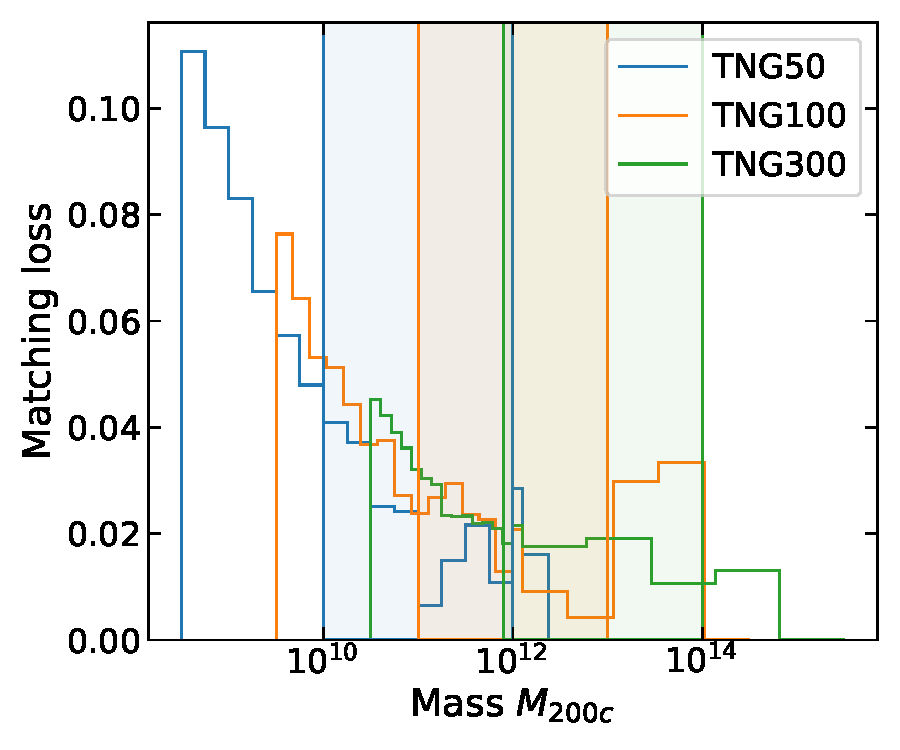
\includegraphics[width=\linewidth]{plots/hal_match_efficiency_mass_all.pdf}
    \caption{Fraction of haloes in the TNG hydrodynamical simulations at $z=0$, that have not found a match is shown as a function of mass $M_{200c}$. Coloured vertical bands represent the mass range relevant for this thesis at $z=0$ in each of the three TNG simulation boxes.}
    \label{fig:matching-loss-all-ch:sims}
\end{figure}

\begin{figure}
\centering
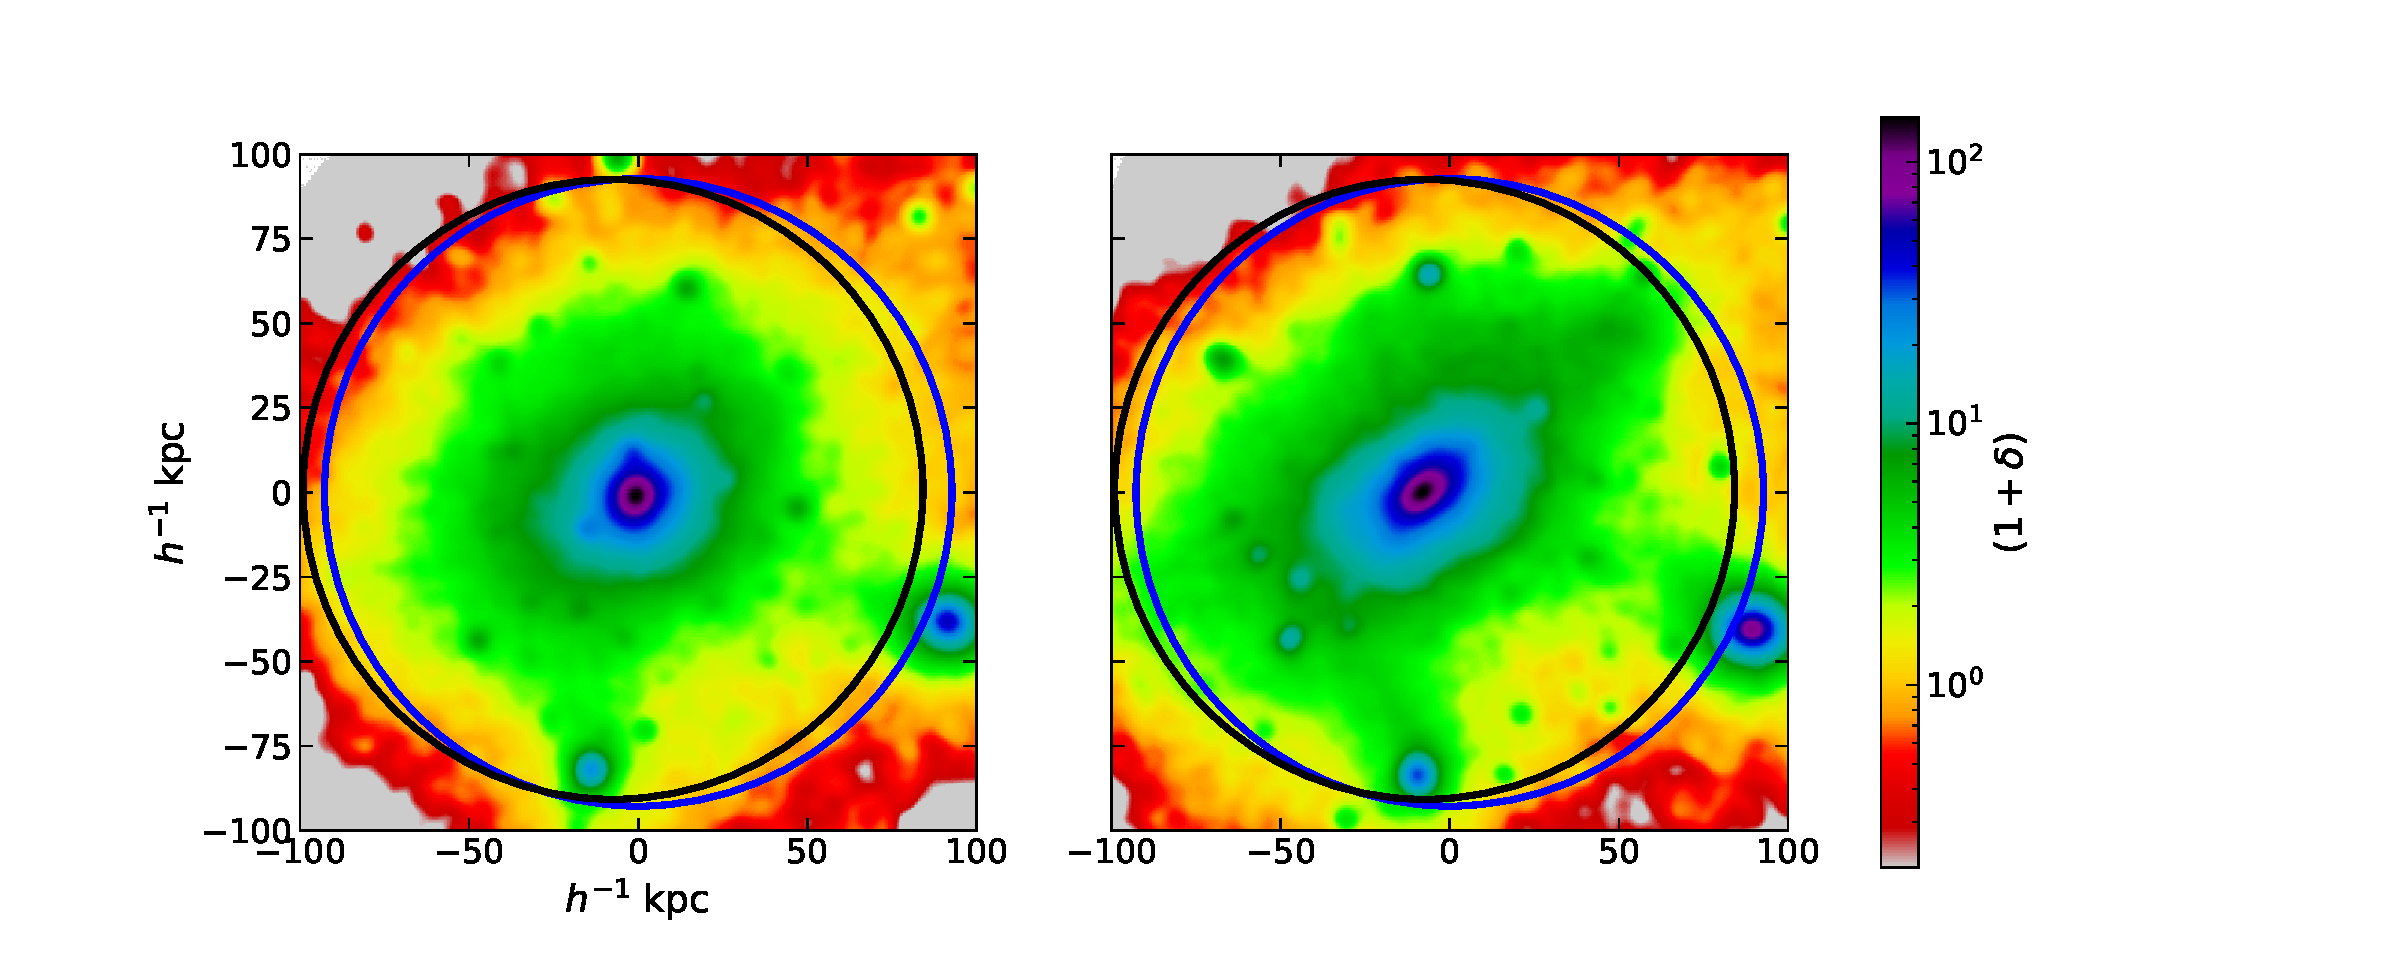
\includegraphics[clip,trim={0.5cm 0cm 2cm 0.5cm}, width=\linewidth]{plots/visual_single_halo.pdf}
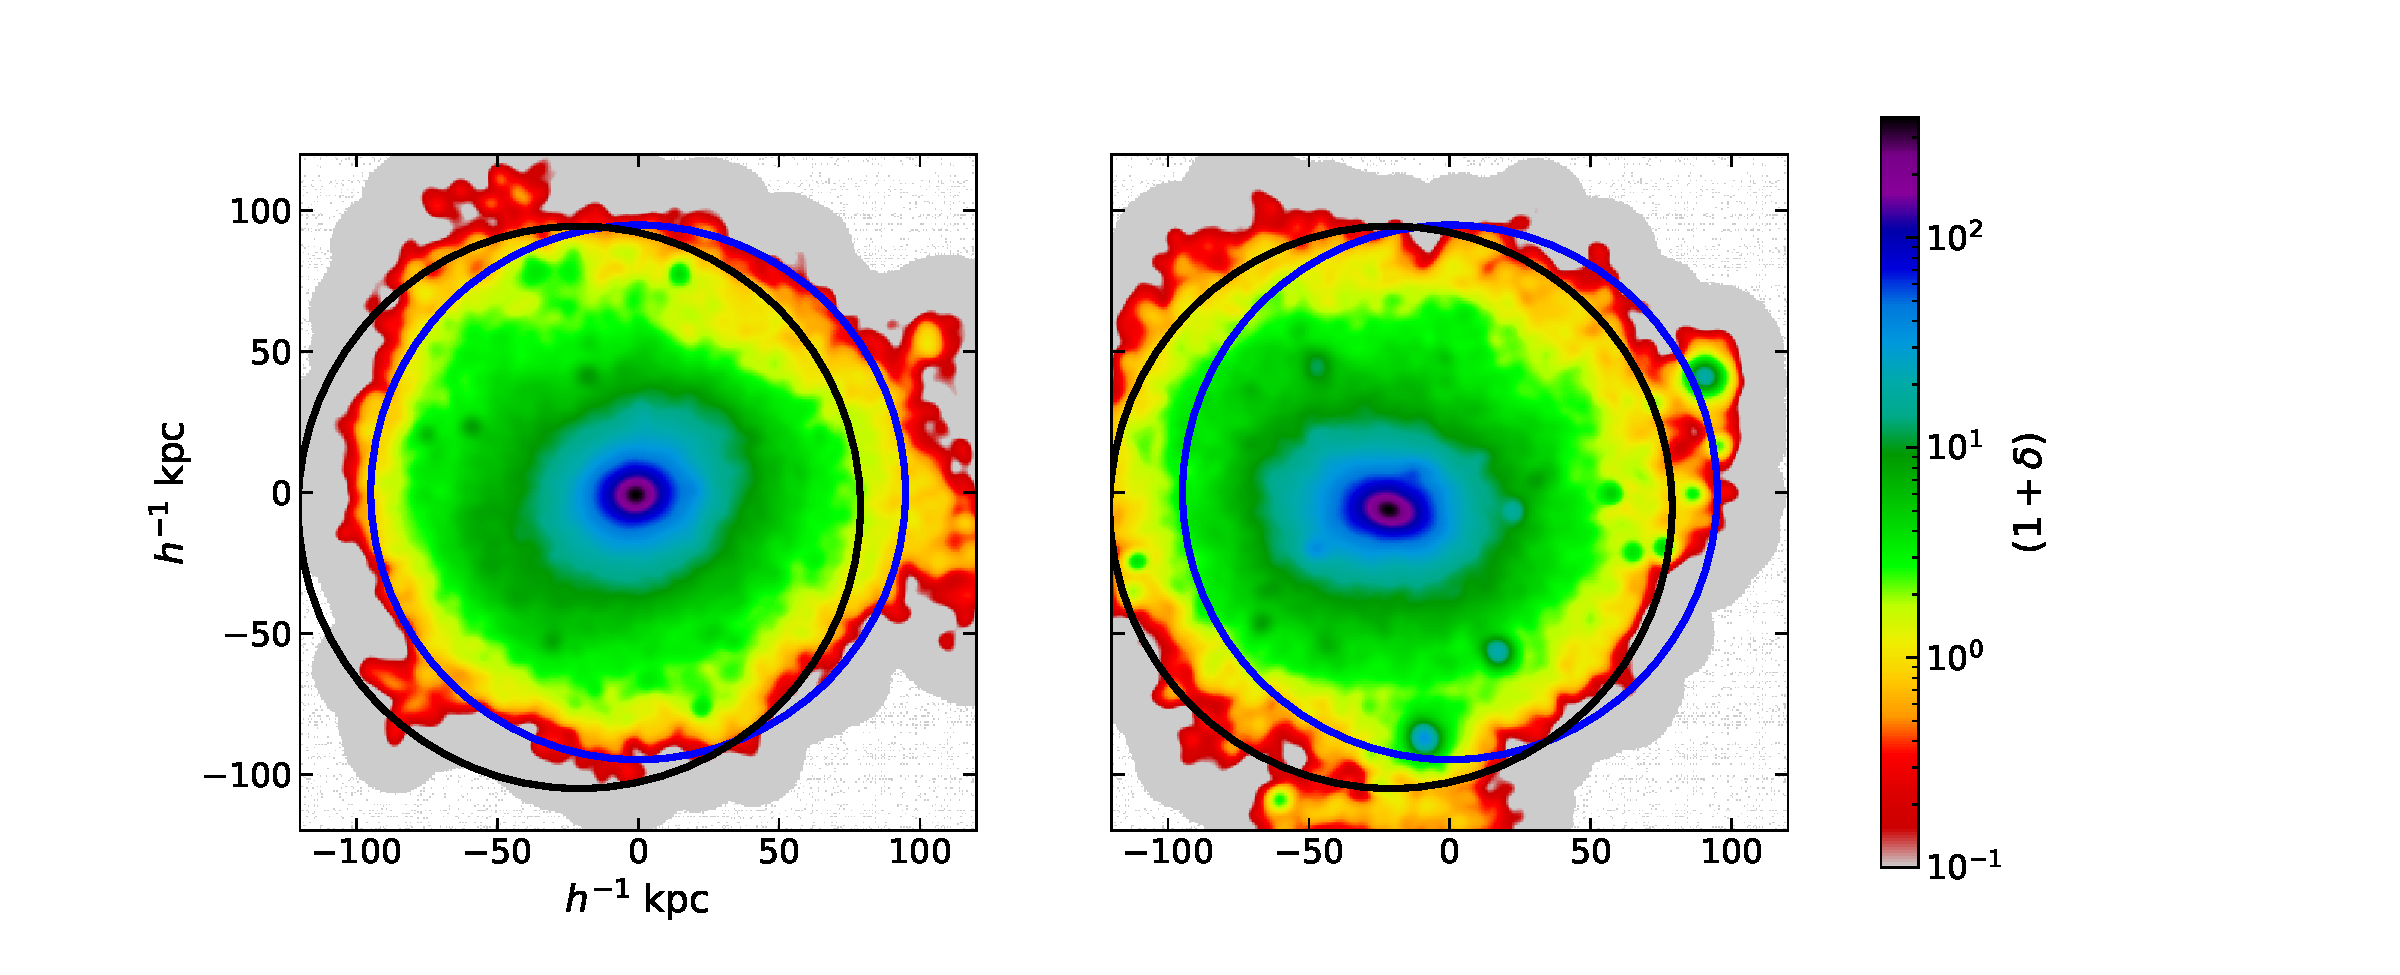
\includegraphics[clip,trim={0.5cm 0cm 2cm 0.5cm}, width=\linewidth]{plots/visual_single_halo_E.pdf}
\caption{Visually inspecting two matched FOF halo pairs, one each from IllustrisTNG \emph{(top row)} and EAGLE \emph{(bottom row)} using 2D-projected dark matter density field around the center of the hydrodynamical halo in a thick slice. The \emph{left panel} shows the halo in the hydrodynamical simulation and the \emph{right panel} shows the corresponding matched pair in the gravity-only simulation. The black circle shows the virial boundary of the gravity-only halo and blue circle shows that of the hydrodynamical halo. In both cases, the hydrodynamical halo is noticeably more spherical and compact than its gravity-only counterpart, with a spatially offset center. See text for a discussion.} 
\label{fig:single-halo-pair-ch:sims}
\end{figure}

Computing the matching fractions 
for every pair of haloes is computationally expensive with $O(n^2)$ for millions of haloes in the catalogue. We decrease the complexity to $O(n)$ by supplying, for each halo in the hydro-simulation, an ordered list of most probable match candidates in the gravity-only run. These candidate lists of gravity-only haloes are generated and ranked based on the spatial positions of the haloes and their masses using a KD-tree based neighbour finding algorithm, implemented using \texttt{scipy.spatial.KDTree}.
For each halo in the hydro run, we test if the matching fraction of this halo with respect to any of the haloes in its match candidate list exceeds the value of 0.5. This ensures that at most one halo is selected as a match for each of the hydrodynamical haloes, so that our matched catalogue of halo pairs will be a subset of the source catalogue without repetitions.
While we match as many haloes as possible, it is also important to ensure that false matches don't plague our study. Based on the results in Appendix \ref{sec:apndx-matching-ch:sims}, we therefore additionally require that in a valid matched pair, the gravity-only FOF halo must also have a matching fraction of more than 0.5 with respect to the hydrodynamical halo.
Our FOF based matching can be compared with
Lovell et al. (2018) \citep[][]{2018MNRAS.481.1950L} where a similar matching algorithm has been followed for central subhaloes.

\subsection{Halo pair catalogue}
We generate a matched catalogue of haloes for all pairs of simulations in this work, including FOF/ROCKSTAR haloes resolved with more than 1000 particles\footnote{Mass resolution in the gravity-only runs are $7 \times 10^7 \Mh$, $8.9 \times 10^6 \Mh$ and $5.4 \times 10^5$ for TNG300, TNG100 and TNG50 respectively; whereas $9.7 \times 10^6 \Mh$ for the L100 and $1.21 \times 10^6 \Mh$ for the L25 simulation of EAGLE.}. The fraction of hydrodynamical haloes that fails to be part of the matched catalogue is shown in \figref{fig:matching-loss-all-ch:sims} in bins of halo mass for the IllustrisTNG simulations. %
In the mass range in which the halo samples are selected for the investigations in this thesis, more than 96\% of the haloes in hydrodynamical simulation have been assigned a match in the gravity-only run. The small fraction of unmatched haloes primarily reside in dense environments 
where our algorithm presumably fails due to
the inherent issues with 3D FOF algorithm in dealing with mergers. Similar results hold for the EAGLE simulations as well. 
For illustrative purpose, a visual representation of two randomly chosen halo pairs, one each from IllustrisTNG and EAGLE, is shown in \figref{fig:single-halo-pair-ch:sims}. 










\section{Characterizing the halo relaxation response}
\label{sec:char_relxn_reln-ch:sims}
The relaxation response in general involves the change in radial and angular distribution of the dark matter within haloes. 
In the illustrative haloes shown in \figref{fig:single-halo-pair-ch:sims}, the change in the radial distribution makes it more compact, while the change angular distribution makes it more spherical in the hydrodynamical simulation that includes galaxy formation. In addition, there is also an offset between the center-of-potential locations of matched pairs of haloes. However, in this thesis we study the former aspect of the halo response, by focusing on spherically averaged mass profiles, leaving the rest for future works.

\subsection{Mass profiles}
\label{subsec:massprofiles-ch:sims}

The overall radial redistribution of dark matter in response to galaxy formation can be studied through the differences in spherically averaged mass profiles between matched haloes. For the dark matter, these radial profiles are obtained by adding up the mass of all dark matter particles contained within concentric spherical shells. In addition to these, we also need baryon mass profiles in modelling the dark matter response. While stellar mass profiles are computed in a similar fashion as dark matter, for the gas mass profiles we use a Gaussian kernel to assign mass enclosed to each of the spherical shells. The width of this Gaussian kernel was taken to match the SPH smoothing length for the EAGLE simulation, whereas for IllustrisTNG and CAMELS we use the cube root of the Voronoi cell volume to define the kernel smoothing scale. We have tested that our results are robust to differences in the choice of this kernel.


\subsection{Quasi-adiabatic relaxation framework}
\label{sec:methods-adiab-ch:sims}
The impact of galaxy formation on the dark halo is expected to be primarily an adiabatic relaxation of dark matter particle orbits in response to baryon condensation \citep[][]{1986ApJ...301...27B}. We start by discussing this simplified model and study more complex effects such as the impact of baryonic feedback processes below.
Assuming that the dark matter halo is spherical and doesn't undergo shell crossing while baryons condense towards the centre, the adiabatic relaxation of any given dark matter shell is determined by the change in baryonic mass within that shell. 
Consider a shell enclosing a \emph{dark matter} mass $M_i^d(r_i)$ in radius $r_i$ in the unrelaxed halo. After relaxation, the radius of the shell changes to $r_f$. By definition, the dark matter mass $M_f^d(r_f)$ enclosed in $r_f$ in the relaxed halo is simply
\be 
M_f^d(r_f) = M_i^d(r_i)\,.
\label{eq:DMmass1}
\ee
The \emph{total} mass $M_i(r_i)$ enclosed in $r_i$ in the unrelaxed halo, on the other hand, does not necessarily equal the total mass $M_f(r_f)$ enclosed in $r_f$ in the relaxed halo.
If angular momentum were to be conserved and the dark matter particle orbits stay circular, then the amount of relaxation of the shell is completely determined by the change in this total mass within the shell
\citep[][]{1986ApJ...301...27B},
\begin{align}
    r_i \,M_i(r_i) = r_f \,M_f(r_f) %
    \implies 
\frac{r_f}{r_i} = \frac{M_i(r_i)}{M_f(r_f)}\,. 
\label{eq:AR1}
\end{align}
Extending this idealised scenario, quasi-adiabatic relaxation models consider the relaxation ratio $r_f/r_i$ as a function of the mass ratio $M_i/M_f$.
\begin{align}
\frac{r_f}{r_i} &= 1 + \chi \left( \frac{M_i(r_i)}{M_f(r_f)} \right) 
\label{eq:qAR1}
\end{align}
For example, the baryonification procedures in \cite{2015JCAP...12..049S,2021MNRAS.503.4147P} include dark matter response as a quasi-adiabatic relaxation with
\be
\chi(y) = q\,(y-1)\,.
\label{eq:chi-linear-ch:sims}
\ee

\subsection{The relaxation relation} %
\label{sec:methods-relx-reln-ch:sims}
Our focus in this thesis is to characterise the relaxation relation \eqn{eq:qAR1} as a function of halo and galaxy properties over a wide dynamic range; e.g, we would like to ask whether \eqn{eq:chi-linear-ch:sims} is a good description of this relation.
To study this, we must extract this relation for individual haloes in hydrodynamical simulations.
For a given hydrodynamical halo in the matched catalog, we can obtain this relaxation relation by considering its matched halo in the gravity-only run to represent its unrelaxed state. 
We find it convenient to work with the relaxed radius, $r_f$ as a control variable. In this case, the values of $r_i$, $M_i(r_i)$ and $M_f(r_f)$ must be obtained from the matched halo pair, which can be done as follows.

For a dark matter shell at radius $r_f$ in the relaxed halo enclosing a dark matter mass of $M_f^d(r_f)$, its unrelaxed radius $r_i$ can be obtained by applying \eqn{eq:DMmass1} and inverting the mass profile $M_i^d(r)=(1-f_b) M_i(r)$ of the gravity-only halo, where $f_b$ is the cosmic baryon fraction, to obtain 
\begin{align}
\label{eq:inv-mass}
r_i = {M_i}^{-1} \left( \frac{M_f^d(r_f)}{(1-f_b)} \right)\,.
\end{align}
This is because each `particle' in the gravity-only halo consists of collisionless baryons and dark matter in precisely the proportion $f_{b}$. 
The value of $M_i(r_i)$ then follows from direct mass counting in the unrelaxed (i.e., gravity-only) halo in radius $r_i$, and the value of $M_f(r_f)$ follows from direct mass counting in the relaxed (i.e. hydrodynamical) halo in radius $r_f$, as described in \secref{subsec:massprofiles-ch:sims}. In practice, we first obtain the unrelaxed mass profile $M_i(r_i)$ for a wide range of radii in finely spaced bins, in order to then compute the inverse in \eqn{eq:inv-mass} by interpolation.

Thus, for any shell defined by its relaxed radius $r_f$, we can obtain both the relaxation ratio $r_f/r_i$ and the mass ratio $M_i/M_f$ from its unrelaxed radius computed from mass profiles. Hence we can obtain the relaxation relation by placing multiple concentric shells around the halo all the way to its virial radius $R_{\rm{vir}}$.
In Appendix \ref{appen:Mock-ch:sims}, we have tested this algorithm on mock halo + galaxy systems generated with fixed known relaxation relations.










\section{Appendix: Choice of matching algorithm}
\label{sec:apndx-matching-ch:sims}
In this thesis, we primarily study the response of dark matter halo to galaxy by comparing the haloes in hydrodynamical simulations to their counterparts in gravity-only runs.
We described the matching procedure in \secref{sec:methods-match-ch:sims}, here we discuss some of the specific choices in that procedure.
For this purpose, let us consider the FOF group haloes in TNG300 simulation with $\log M(\Mh)>10.5$.  There are 543588 FOF groups satisfying this criterion in the hydrodynamical run of TNG300, with each of them having more than 500 particles within their $R_{\rm vir}$ in the highest resolution run.
Following the matching procedure described in \secref{sec:methods-match-ch:sims} (requiring only that the matching fraction of the hydrodynamical halo with respect to the gravity-only halo is greater than 0.5), we get a matching halo in the gravity-only run for 541594 of them, leaving out only 1994 haloes unmatched, that is a negligible 0.4\% spread across the mass range (\figref{fig:efficiency-mass-ch:sims}).
However, if we follow the same procedure using matching fraction between the central subhaloes instead of FOF group themselves, then we get a order of magnitude more unmatched haloes as can be seen in the \figref{fig:efficiency-mass-ch:sims}.  

\begin{figure}
    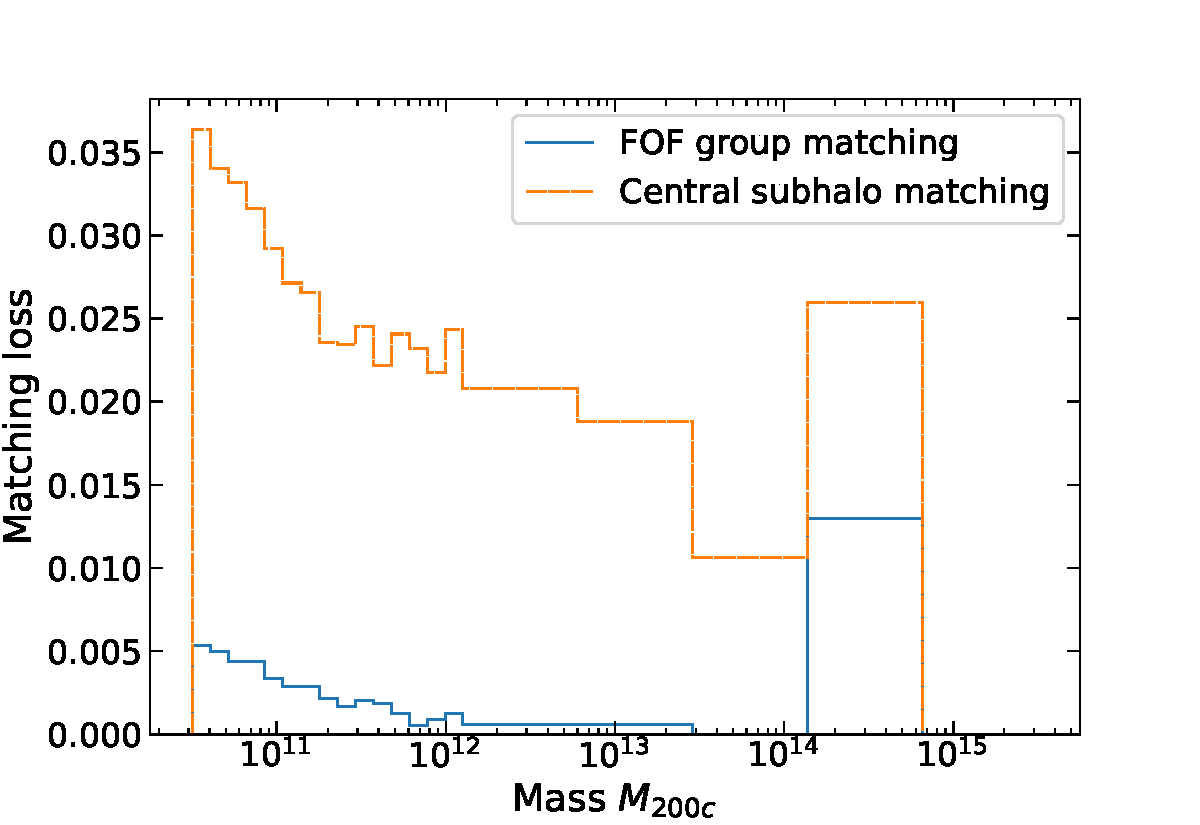
\includegraphics[width=\linewidth]{plots/hal_match_efficiency_mass.pdf}
    \caption{Fraction of haloes in the TNG300-1 hydrodynamical simulation that have not found a match is shown as a function of mass $M_{200c}$.}
    \label{fig:efficiency-mass-ch:sims}
\end{figure}

\begin{figure}
\centering
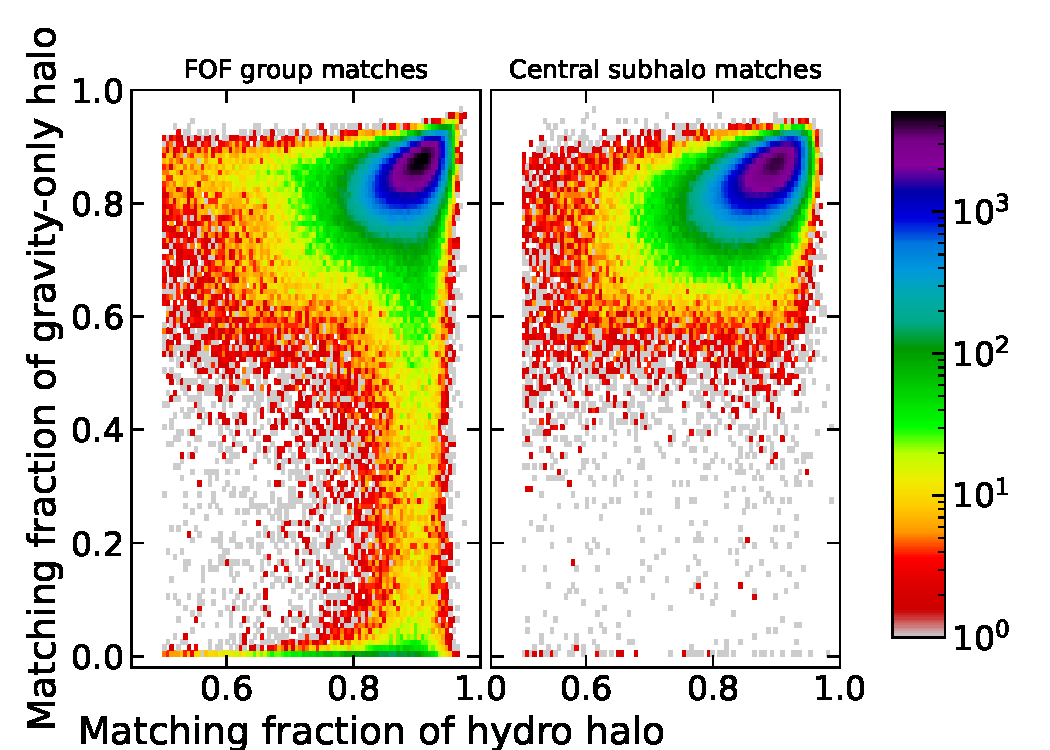
\includegraphics[width=\linewidth]{plots/hal_match_accuracy_hist2d.pdf}
\caption{Histogram of matching accuracy of haloes in the FOF group matched catalogue (left) and central subhalo matched catalogue (right). The x-axis is the fraction of dark matter particles in the hydrodynamical halo that is also in the gravity-only halo.}
\label{fig:accuracy-hist2d-ch:sims}
\end{figure}

\begin{figure}
    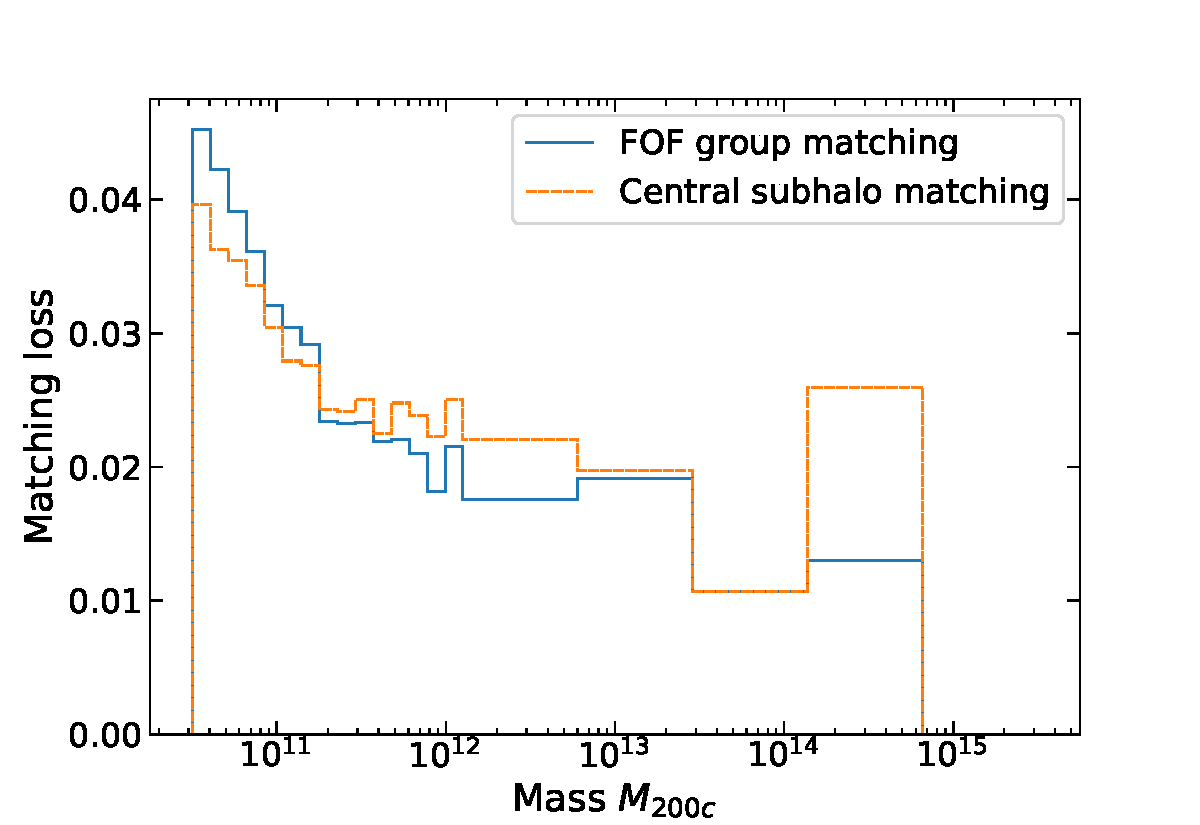
\includegraphics[width=\linewidth]{plots/hal_match_efficiency_mass_rev.pdf}
    \caption{Fraction of haloes in the TNG300-1 hydrodynamical simulation that have not found a match is shown in left panel as a function of mass $M_{200c}$ after removing asymmetrical matches (see text in appendix \ref{sec:apndx-matching-ch:sims}.}
    \label{fig:efficiency-mass-rev-ch:sims}
\end{figure}

While obtaining matches for as many haloes as possible, we also have to ensure the quality of match. To check how well the haloes in each of the pairs in our catalogue are matching we look at the particle matching fraction of each halo in the pair with respect to the other as shown in \figref{fig:accuracy-hist2d-ch:sims}. By definition the gravity-only halo in every pair has atleast 50\% of the dark matter particles of the hydrodynamical halo in that pair. But note that in FOF group matching based catalogue, for a significant number of pairs the hydrodynamical halo in the pair has less than 10\% of the gravity-only halo's particles. By visually inspecting some of those halo pairs we find that, they represent haloes with ongoing merger events. This explains the significant loss in matching efficiency when we used central subhalo matching. 

In the \figref{fig:efficiency-mass-rev-ch:sims}, matching loss as a function of halo mass is shown after removing all those pairs in which the particle matching fraction of the gravity-only halo with respect to hydrodynamical halo is less than 50\%. Since this symmetrical matching condition produces consistent matched catalogue of haloes, we apply this additional matching condition  but stick to matching whole FOF groups. With this procedure, our final matched catalogue for TNG300 contains 524841 pairs, leaving 18747 out of 543588 hydrodynamical haloes unmatched. The additional unmatched haloes primarily reside in dense environments, and we can't find match for those haloes because of the inherent issues with 3d FOF algorithm in dealing with mergers. 


\section{Appendix: Mock particles in a Galaxy-Halo system}
\label{appen:Mock-ch:sims}
Here we validate our method used in extracting the relaxation relation (see \secref{sec:methods-relx-reln-ch:sims}) using mock galaxy-halo systems.
In this, we use Hernquist profile for the initial unrelaxed dark matter halo and similar analytical mass profiles for the baryon components \citep[see appendix of][]{2021MNRAS.507..632P}. We then get the relaxed dark matter profile using quasi-adiabatic relaxation model with different values of $q$. Mock particle data is then generated with these mass profiles for different components of hydrodynamical halo and the corresponding gravity-only halo.

\begin{figure*}
    \centering
    (a) Mass profiles\\
    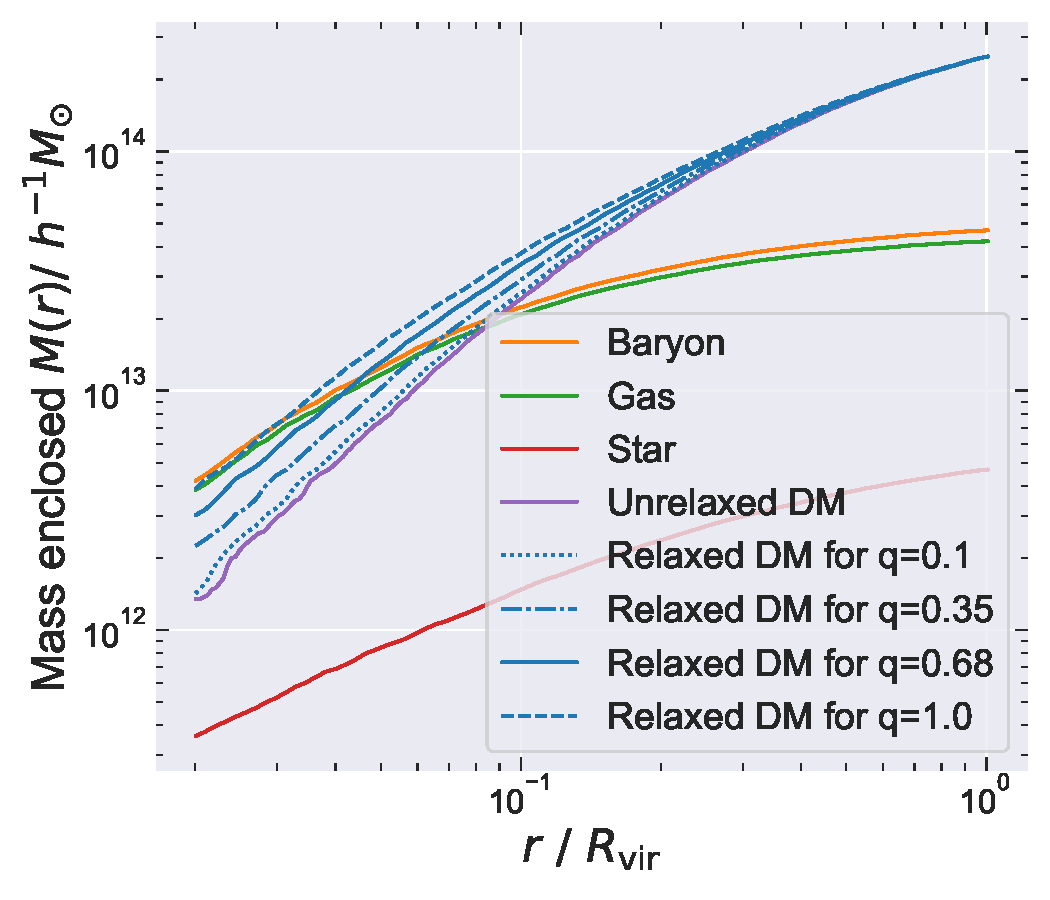
\includegraphics[clip,trim={0.2cm 0.5cm 0.4cm 0cm}, width=0.49\linewidth]{plots/mock_stargas_N=10000-Mr}
    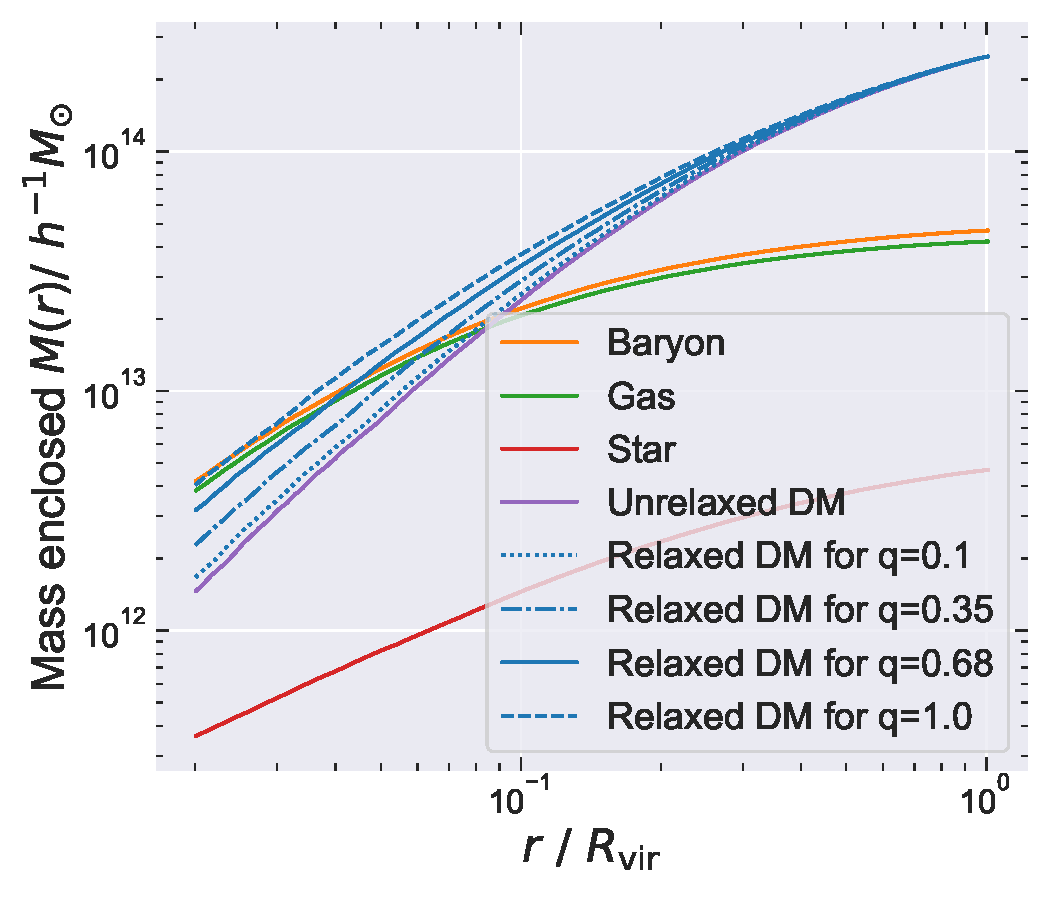
\includegraphics[clip,trim={0.2cm 0.5cm 0.4cm 0cm}, width=0.49\linewidth]{plots/mock_stargas_N=100000-Mr}
    (b) Relaxation ratio\\
    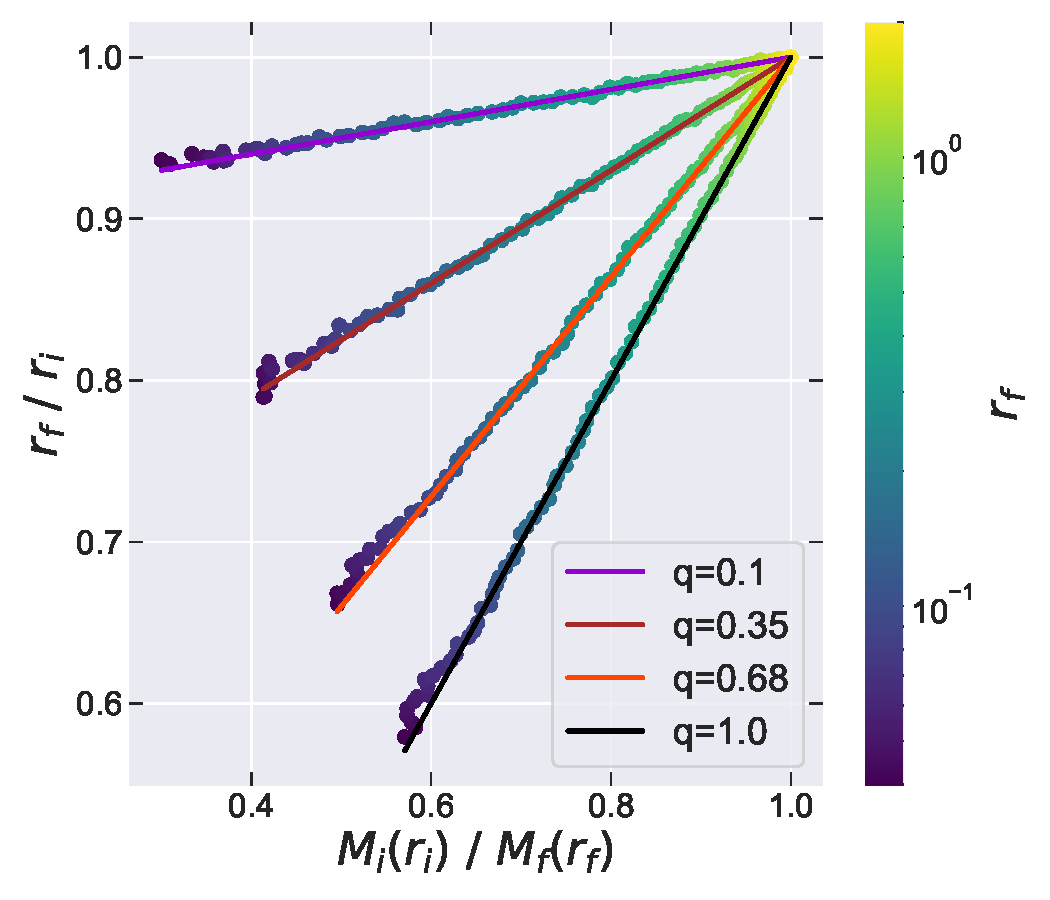
\includegraphics[clip,trim={0.2cm 0.5cm 0.4cm 0cm}, width=0.49\linewidth]{plots/mock_stargas_N=10000-ratio}
    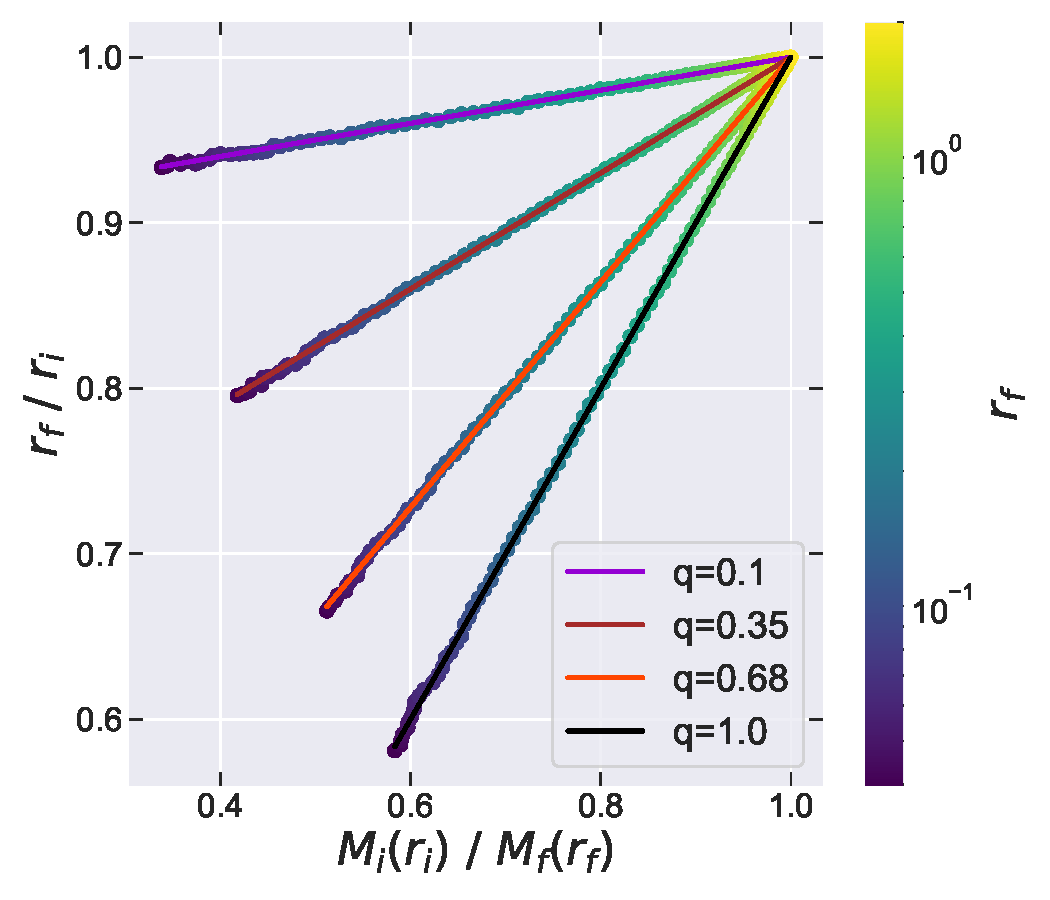
\includegraphics[clip,trim={0.2cm 0.5cm 0.4cm 0cm}, width=0.49\linewidth]{plots/mock_stargas_N=100000-ratio}
    \caption{Mock halo with Hernquist profile for unrelaxed dark matter and with the analytical baryon mass profile from \citet{2021MNRAS.507..632P} for gas and star components. The relaxed dark matter profile is modelled by quasi-adiabatic relaxation with different choices of q parameter. Haloes are sampled by \textbf{$10^4$} particles in left panel and \textbf{$10^5$} particles in the right panel.
        (a) Mass enclosed within spherical shell as a function of the shell radius for different components. 
        (b) Relaxation ratio as a function of the ratio of total mass enclosed. The linestyle indicate the different values for the model parameter $q$ used in generating the mock data, while the colourbar shows the final radius. While the solid lines represent the expected relaxation relation for each case, the colored markers show the computed relaxation relation from the mock particle data parametrized by the relaxed radius in units of the virial radius.}
    \label{fig:mock-ch:sims}
\end{figure*}

For those mock halo pairs, we compute the mass profiles and obtain the relaxation ratio as a function of the dark matter shell radius as discussed in \secref{sec:char_relxn_reln-ch:sims}. We then repeat this for mock halo pairs generated with different particle resolutions. We find that the computed relaxation relation shown by colored markers matches with expected relaxation relation shown in solid lines; however, the choice of radial bins is limited by the particle resolution (see \figref{fig:mock-ch:sims}).
% \section{Haloes}

% \section{Characterizing the halo response}

\chapter[The quasi-adiabatic relaxation of haloes in the IllustrisTNG and EAGLE cosmological simulations at z=0]{The quasi-adiabatic relaxation of haloes in the IllustrisTNG and EAGLE cosmological simulations at $z=0$}
\label{chap:z0_main}
% \section{Introduction}
% \label{sec:intro-ch:z0main}
% \noindent

In this chapter, we perform a systematic, statistical study of the response in the radial distribution of dark matter due to baryonic processes with haloes identified in high-resolution cosmological simulations of galaxies. We perform this study at the present epoch (\(z=0\)) in the main simulations from the IllustrisTNG \citep[][]{2019ComAC...6....2N} and EAGLE \citep[][]{2017arXiv170609899T} suites. This includes TNG300, TNG100, and TNG50 simulated with the reference TNG model, and L0100N1504 and L025N0752 (denoted L100 and L25, respectively) simulated with the reference EAGLE model. These two different models of baryonic evolution include different subgrid prescriptions for various astrophysical processes. However, they both have produced state-of-the-art galaxies in the cosmological setting. Hence, all these simulations are expected to capture a reasonably accurate description of the backreaction on the dark matter haloes; see \secref{sec:sims} for details.

We isolate the effects of the galaxy formation process on dark matter haloes identified in these hydrodynamical simulations by comparing them against their matched partner haloes from their corresponding gravity-only runs that evolve the same initial cosmological volumes (see \secref{sec:hals} for details). In particular, we focus on the differences in the radial distribution for each of these halo pairs, characterized by the relaxation relations described in \secref{sec:char_relxn_reln-ch:sims}.

We begin by exploring the relaxation relations in a variety of individual halo pairs in \secref{sec:results-1-ch:z0main}. By stacking these relations in a population of haloes, we could capture the average relaxation behavior in the population. This allows us to study the dependence of relaxation on specific physical quantities of interest by excluding the statistical variation between individual haloes. In \secref{sec:results-mass-ch:z0main}, we study these stacked relaxation relations in populations of haloes selected within narrow bins of halo masses from $10^{10} \Mh$ to $10^{14} \Mh$.

While these stacked relations could be directly compared against existing quasi-adiabatic relaxation models such as Abadi et al. (2010) \citep{2010MNRAS.407..435A}, they are harder to interpret quantitatively. Instead, we demonstrate in \secref{sec:results-rad-dep-qadiab-ch:z0main} that considering an explicit dependence on the halo-centric distance allows a simple and accurate description of the relaxation behavior in halo populations. Using this method, we characterize the dependence of the dark matter relaxation response on a variety of relevant halo and galaxy properties in \secref{sec:dep-on-hal-gal-props-ch:z0main}.

These results are expected to be relevant for a variety of problems; for example, the change in the dark matter density profile of the halo caused by the galaxy formation affects the rotation curve of the galaxy. We discuss such applications in \secref{sec:applic-ch:z0main} and conclude in \secref{sec:conclusion-ch:z0main}. 





% \section{Results}
% \label{sec:results-ch:z0main}


\section{Relaxation of Haloes in the IllustrisTNG}
\label{sec:results-1-ch:z0main}

We find that the relaxation relation $r_f/r_i$ vs. $M_i/M_f$, estimated as described in \secref{sec:char_relxn_reln-ch:sims}, varies widely across haloes in the matched catalogue. In \figref{fig:relx-results-simple-ch:z0main}, we show the relaxation relation for four different samples of haloes selected by their unrelaxed mass from the IllustrisTNG simulations. 

The first two samples are from TNG50, with masses $M \sim 10^{11.5} \Mh$ and $10^{12} \Mh$, respectively. Similarly, the other two samples are from TNG100 and TNG300, with masses $M \sim 10^{12.5} \Mh$ and $10^{13.5} \Mh$, respectively. The relaxation relations of a few individual randomly chosen haloes from each sample are shown by grey lines; we also show stacked relaxation relations for each sample (see below for measurement details). The quasi-adiabatic relaxation model \eqn{eq:chi-linear-ch:sims} with $q=0.68$ and $q=0.33$ is shown by the dot-dashed and dashed purple lines, respectively, in each panel. The value $q=0.68$ was proposed by Schneider $\&$ Teyssier (2015) \citep{2015JCAP...12..049S} as being a reasonable description of cluster-sized haloes, while Paranjape $\&$ Sheth (2021) \citep{2021MNRAS.507..632P} argued that $q=0.33$ leads to a good description of the radial acceleration relation of Milky Way-sized spiral galaxies (see their Appendix A1). We will use these two models as reference points in the comparisons below. Since the samples shown are representative of the haloes in IllustrisTNG over a large mass range, it is clear that \emph{\eqn{eq:chi-linear-ch:sims} with a constant $q$ does not work for the majority of haloes in IllustrisTNG.} Similar results hold for EAGLE haloes as well. This motivates a systematic study of the relaxation relation as a function of halo mass and other properties.

For each of the four samples selected by halo mass, we compute the relaxation ratio $r_f/r_i$ and the enclosed total mass ratio $M_i/M_f$ at 20 concentric spherical shells for all haloes in the sample. We take the largest shell at the relaxed virial radius $r_f=R_{\rm{vir}}$, while the remaining 19 shells are taken at fixed values of $r_f/R_{\rm{vir}}$ for each halo. This allows us to stack the relaxation relation by simply taking the mean and standard deviation of the relaxation ratio and mass ratio at each of the 20 shells. While the physical size of the shell differs from halo to halo, we ensure that the smallest shell has a radius of at least 10 times the force smoothing length of the simulation. In \figref{fig:relx-results-simple-ch:z0main}, we show this stacked relaxation relation in large coloured markers, where the colour denotes the relaxed radius of the shell; and the error bar shown in red corresponds to the statistical error in the estimate of the mean value. By comparing with the small markers of the same colour, we can see that there is significant scatter not only in the relaxation ratio but also in the mass ratio at fixed $r_f/R_{\rm{vir}}$ across haloes in each sample.

To assess the level of systematic error introduced by our default choice of stacking technique, we also tested an alternate stacking definition, wherein we interpolate the relaxation relation of individual haloes to obtain the relaxation ratio at fixed values of mass ratios and stack them by ignoring the value of corresponding relaxed radii. However, this stacking method ignores radius information completely; we discuss the consequences of this later in \secref{sec:results-rad-dep-qadiab-ch:z0main}.

\begin{figure}
    \centering
    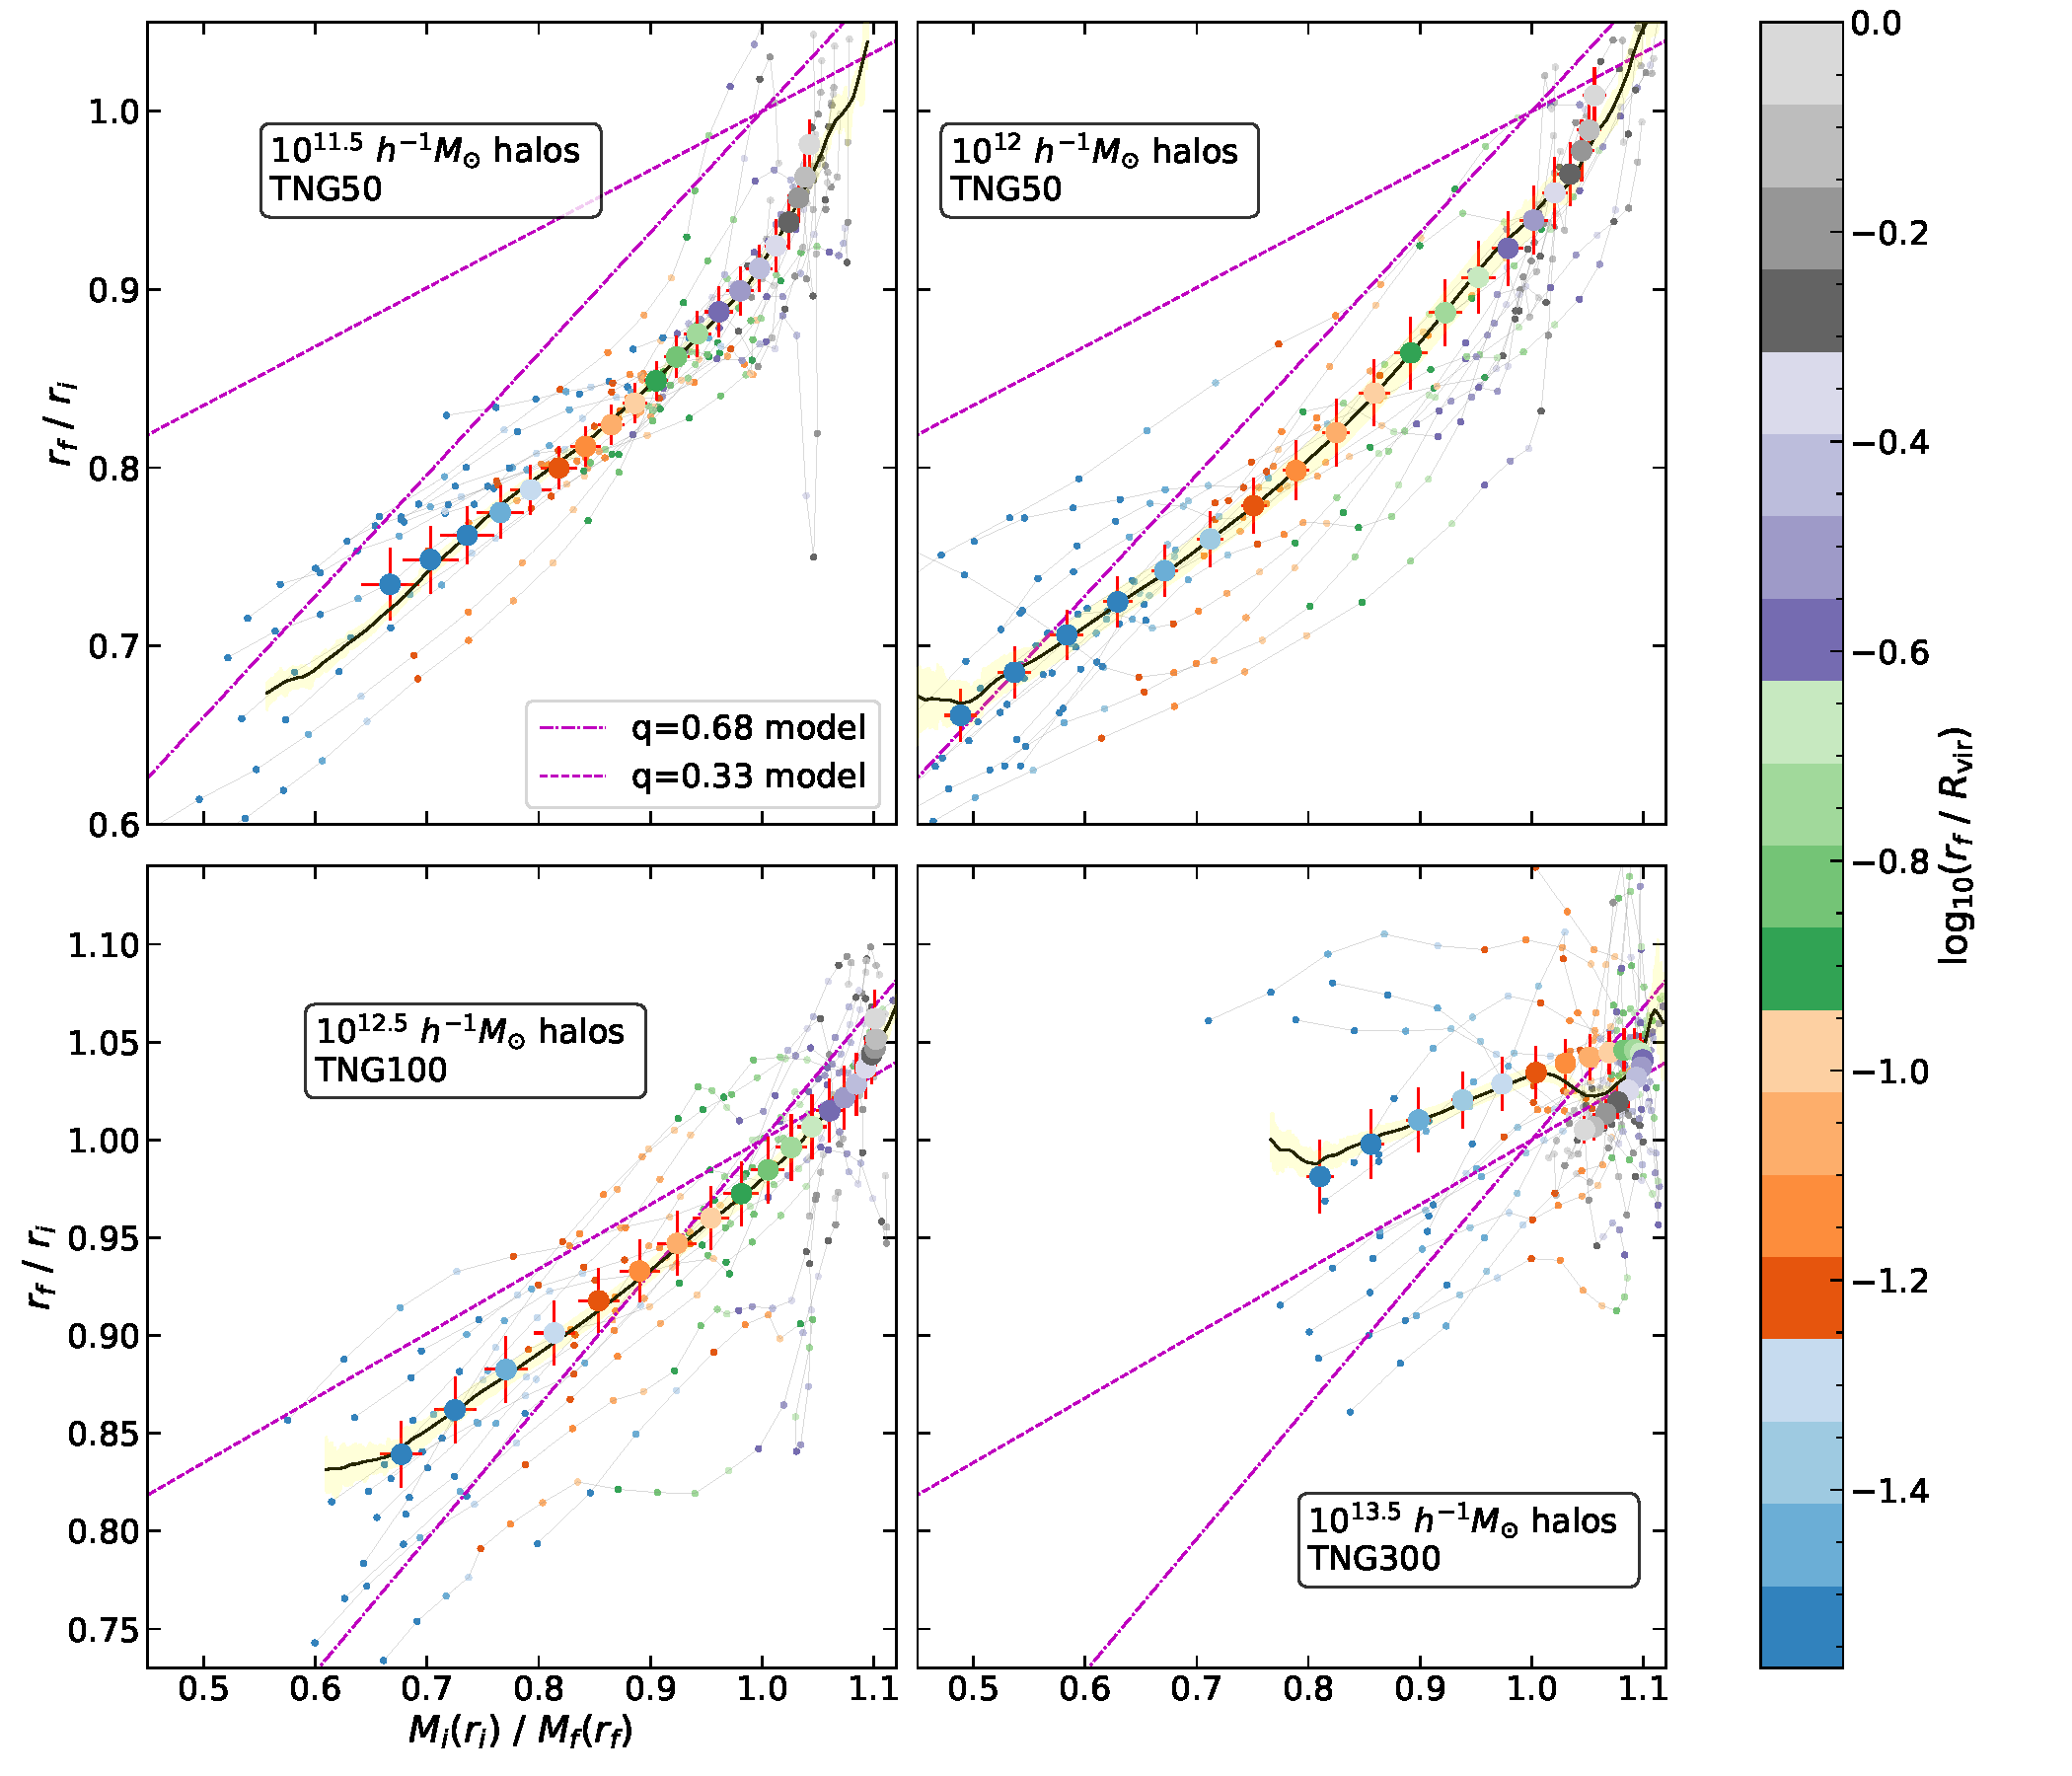
\includegraphics[width=\linewidth,trim={0 0 0cm 0},clip]{plots/indv_relx-reln_all.pdf}
    \caption{Relaxation relation for 4 different samples of haloes selected by mass from the IllustrisTNG simulations. The large coloured circles denote the stacked relaxation ratio and total mass ratio at 20 different shells, whose radii are indicated by the colour. Small coloured markers joined by grey lines show the relaxation relation of a few randomly chosen individual haloes in each of the samples. The black curves denote the radius-independent stack of the relaxation relation for each sample (see text). The quasi-adiabatic relaxation model \eqn{eq:chi-linear-ch:sims} with $q=0.68$ and $q=0.33$ are shown by the dot-dashed and dashed purple lines, respectively, in each panel.} 
    \label{fig:relx-results-simple-ch:z0main}
\end{figure}




\section{Trend in relaxation relation with halo mass}
\label{sec:results-mass-ch:z0main}
As can be already noted in \figref{fig:relx-results-simple-ch:z0main}, the relaxation relation shows very different behaviour at different mass scales. In this section, we focus on the stacked relation (using our default stacking definition) and study how it varies as a function of unrelaxed halo mass. For this, we consider nine mass bins starting from $\log (M/\Mh) = 10$ to $14$ in steps of $0.5$ dex. We list the colour labels used for these mass bins in \figref{fig:mass_bin_label-ch:z0main}; this colour-coding will be used in all subsequent plots. None of the five simulations considered, simultaneously provides a sufficiently large sample of cluster-scale haloes and well-resolved low-mass haloes.
In the IllustrisTNG suite, we use the smallest box TNG50 to study haloes with mass $10^{10} \Mh < M < 10^{12} \Mh$, whereas we use TNG100 and TNG300 to study haloes with mass $10^{11} \Mh < M < 10^{12.5} \Mh$ and $10^{12} \Mh < M < 10^{14} \Mh$ respectively. At those mass bins where multiple IllustrisTNG boxes provide halo samples, the smaller box provides a smaller sample but with better resolution. For computational ease, we limit the size of each sample to be $\leq500$ haloes, as we find that the statistics are well-converged with this number.

\begin{figure}
    \centering
    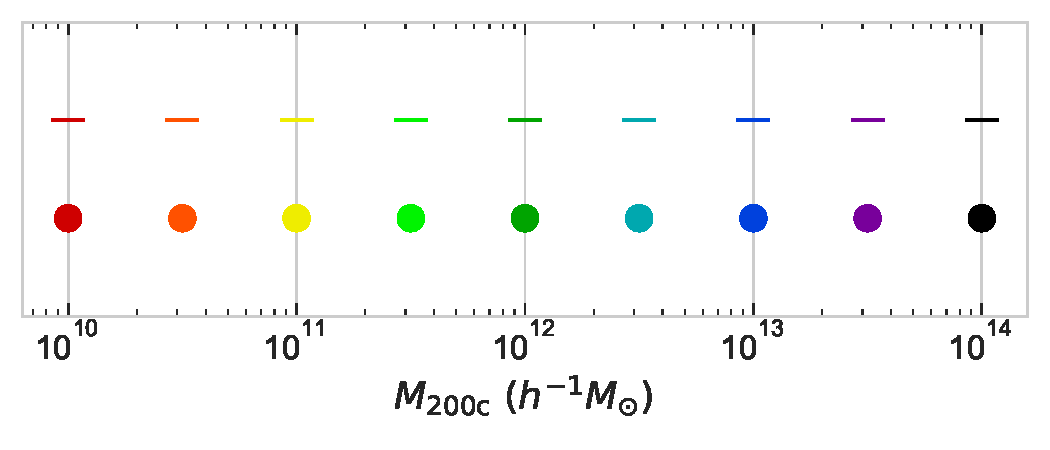
\includegraphics[width=0.69\linewidth]{plots/Mass_bin_labels.pdf}
    \caption{Representative colours we use to denote each of the halo mass bins.}
    \label{fig:mass_bin_label-ch:z0main}
\end{figure}

By repeating the procedure described in \secref{sec:results-1-ch:z0main}, we obtain both the fixed-radius (default) stack and radius-independent (alternate) stack of the relaxation relation for each of the halo samples taken from IllustrisTNG at these nine mass bins (see \emph{left panel} of \figref{fig:fit-view-mass-indep-ch:z0main}). 
For reference, note that the case of no relaxation would correspond to a horizontal line at unity in this plot.
Relaxation is strongest for Milky Way-scale haloes, as indicated by the small values of the relaxation ratio for $M\sim10^{12}\Mh$; we discuss the physical implications of this result later. 
Note that the simple quasi-adiabatic relaxation model \eqn{eq:chi-linear-ch:sims} with $q=0.68$ \citep{2015JCAP...12..049S} fails to explain the relaxation relation for any of the halo masses considered; however this model with $q=0.33$ is reasonably close to the relaxation relation at %
$M\sim 10^{13} \Mh$. 
And while the quadratic model proposed by Abadi et al. (2010) \citep{2010MNRAS.407..435A} matches with the relaxation relation of $10^{12.5} \Mh$ haloes in IllustrisTNG, this is possibly a coincidence given that this model was built using zoom simulation of haloes in the mass range $10^{11.5} $-$ 10^{12} \Mh$, which show a very different relaxation relation in IllustrisTNG.\footnote{The simulation used by Abadi et al. (2010) \citep{2010MNRAS.407..435A} also suffered from overcooling due to the lack of feedback effects, so that the mass ratios attained much smaller value for shells at the same radii as compared to IllustrisTNG.}

\begin{figure}
\centering
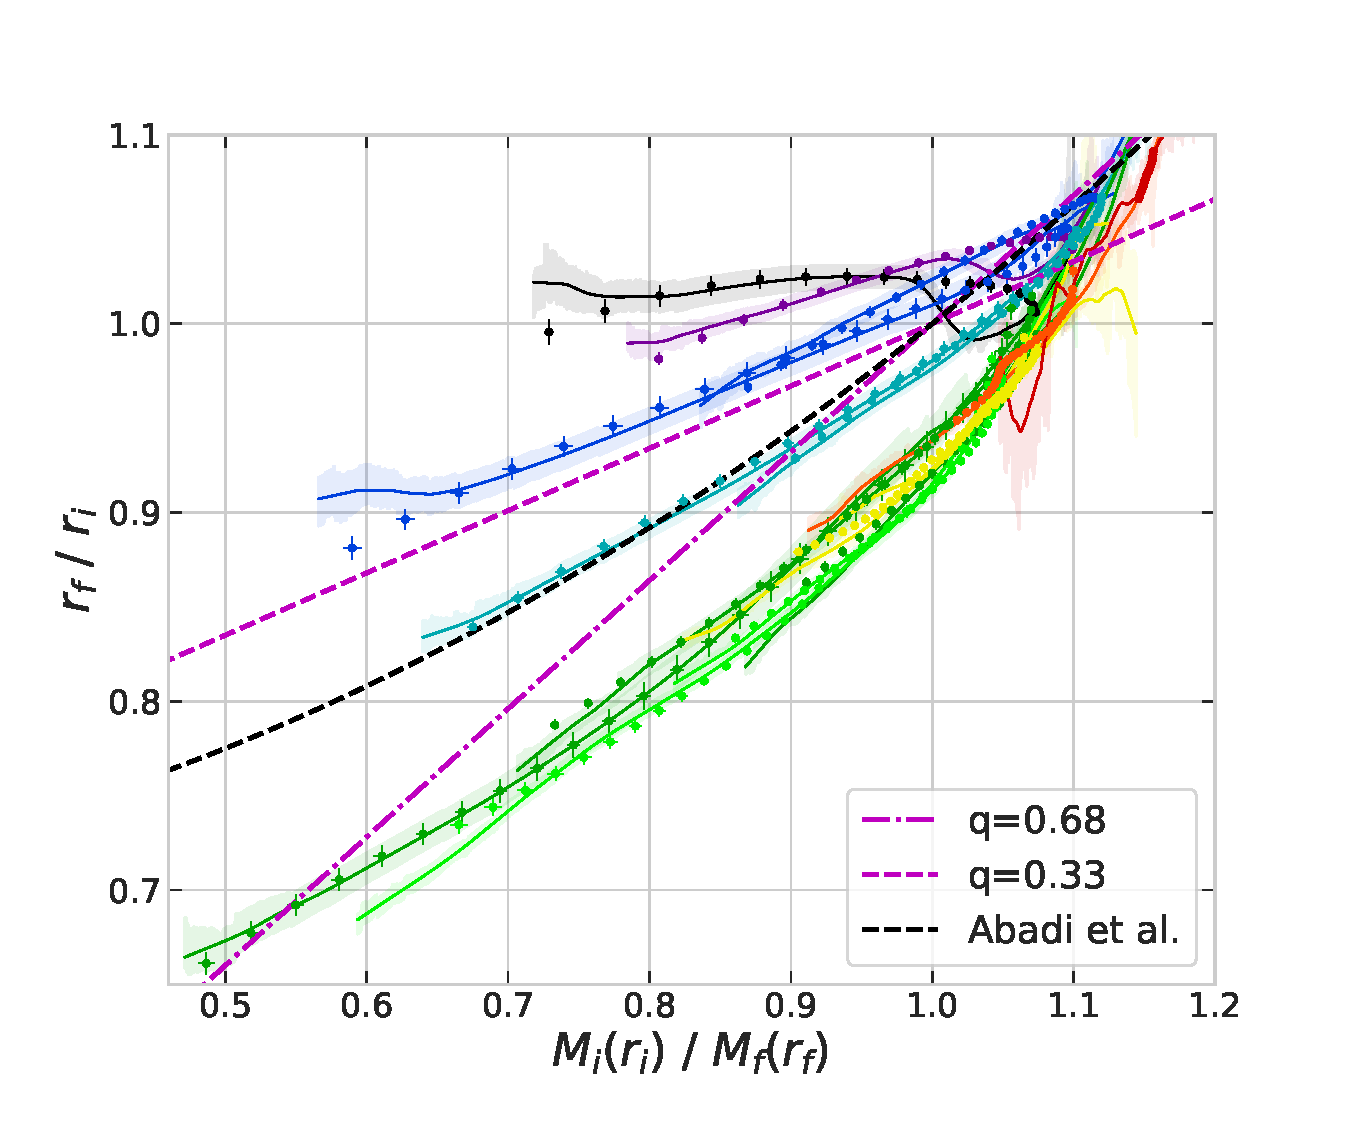
\includegraphics[width=0.49\linewidth]{plots/fit_view_M_T.pdf}
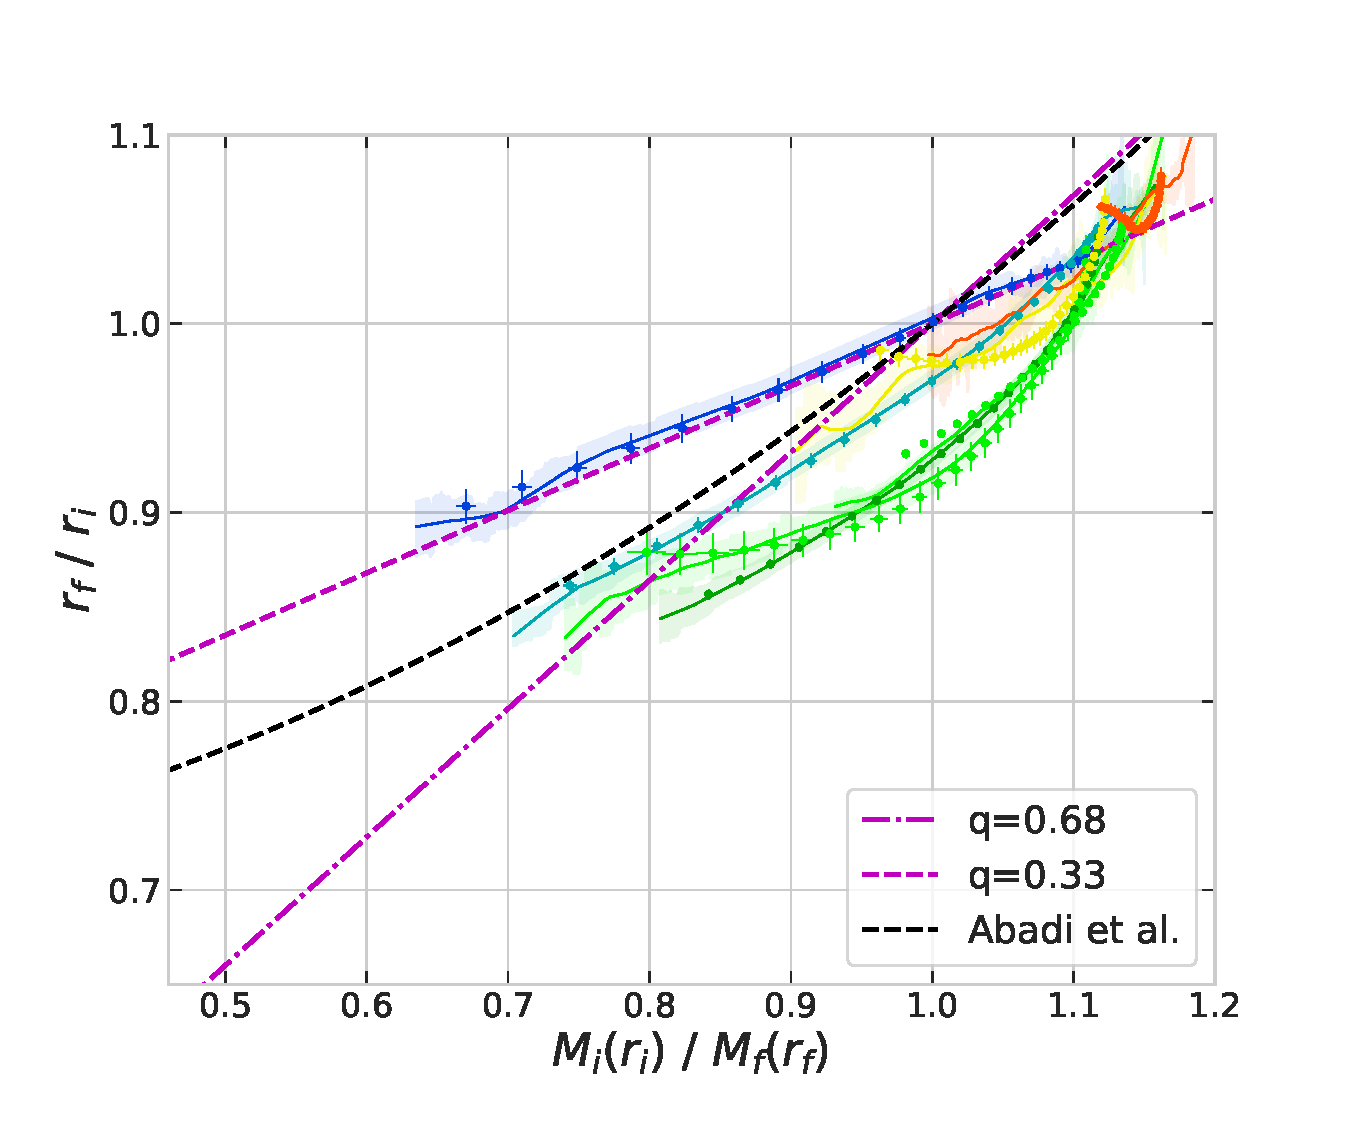
\includegraphics[width=0.49\linewidth]{plots/fit_view_M_E.pdf}
\caption{The stacked relation between relaxation ratio and mass ratio as a function of halo mass in IllustrisTNG (left panel) and EAGLE (right panel) simulations. Here the points and solid lines represent two different stacking methods as in Fig.~\ref{fig:relx-results-simple-ch:z0main}. The colour-coding follows Fig.~\ref{fig:mass_bin_label-ch:z0main}.} 
\label{fig:fit-view-mass-indep-ch:z0main}
\end{figure}








We also take six samples of haloes from the EAGLE simulation, in mass bins $\log (M/\Mh) = 10.5, 11,11.5$  from the small, high-resolution L25 box and in mass bins $12, 12.5, 13$ from the main L100 box. Here too, the $q=0.68$ model fails for all masses, but $q=0.33$ model works reasonably for  $M\sim10^{13} \Mh$ haloes (see the \emph{right panel} of \figref{fig:fit-view-mass-indep-ch:z0main}). We find that, despite having a different galaxy formation model, the relaxation relation for haloes found in the primary EAGLE run L100 is consistent with the results from IllustrisTNG. 
IllustrisTNG samples reach lower values of the relaxation ratio and mass ratio than EAGLE because of the better resolution available. For $M_{200}=10^{12} \Mh$, the mean relaxation relation shown in \figref{fig:fit-view-mass-indep-ch:z0main}, does not seem to be very different between IllustrisTNG and EAGLE $L100$, atleast not anymore than the difference between different boxes of the IllustrisTNG. However, the haloes from EAGLE $L25$ simulation shows a unique behaviour where the relaxation ratio increases with decrease in mass ratio in the innermost regions. We expect that this might be due to the fact that the EAGLE reference model required recalibration at this higher resolution. In a future work we will explore how the dark matter response depends on such variations in the baryonic prescription.


\section{Parametrised model of quasi-adiabatic relaxation}
\label{sec:results-rad-dep-qadiab-ch:z0main}
In this section, we model the relaxation relations discussed above, with a focus on conveniently quantifying this response across a wide range of halo masses.



\subsection{Expectations from simulation measurements}
\label{subsubsec:sim-relax-ch:z0main}
In both IllustrisTNG and EAGLE, for all masses other than $10^{13} \Mh$, the simple quasi-adiabatic relaxation model \eqn{eq:chi-linear-ch:sims} fails to explain the measured relation with any value of $q$. 
As seen in Fig.~\ref{fig:fit-view-mass-indep-ch:z0main}, an important aspect of this mismatch is caused by the model's requirement that shells which hold their baryonic mass fixed (i.e., for which $M_i/M_f=1$) must necessarily also hold their radius fixed ($r_f/r_i=1$), and vice-versa. The measurements, however, show substantial offsets in the relaxation ratio from unity for shells with $M_i/M_f = 1$, and also substantial offsets in the mass ratio from unity for shells with $r_f/r_i=1$, across nearly the entire range of halo mass. One way of understanding this effect physically is due to feedback-related baryonic outflows: a particular shell which maintains its radius after relaxation ($r_f/r_i=1$), could still lose its baryonic mass due to outflows, resulting in $M_i/M_f > 1$ \citep[][]{2022MNRAS.511.3910F}. Alternatively, the interplay between cooling-related condensation (which increases baryonic mass in a given shell) and feedback-related outflows (which decrease baryonic mass) could result in a situation where the baryonic mass after relaxation retains its initial value despite an overall relaxation, e.g. due to approximate angular momentum conservation, leading to $r_f/r_i < 1$ while $M_i/M_f=1$. These trends are visible  in  Fig.~\ref{fig:fit-view-mass-indep-ch:z0main}  for haloes with $M<10^{13}\Mh$. Fig.~\ref{fig:relx-results-simple-ch:z0main} shows that the former trend ($M_i/M_f > 1$ when $r_f/r_i=1$) occurs in the halo outskirts ($r_f\sim R_{\rm vir}$) and the latter ($r_f/r_i < 1$ when $M_i/M_f=1$) in the inner halo ($r_f\lesssim0.3\,R_{\rm vir}$), for $M<10^{13}\Mh$. 
On the other hand, more massive haloes show little to no relaxation in both inner halo (where there is net baryonic inflow, $M_i/M_f < 1$) and outer halo (where there is net baryonic outflow, $M_i/M_f > 1$).

To account for such effects, we expand the simple quasi-adiabatic relaxation model \eqn{eq:chi-linear-ch:sims} by adding 
a null offset parameter $q_0$:
\begin{align}
    \label{eq:chi-linear-q0-ch:z0main}
    \frac{r_f}{r_i} - 1 &= q_1 \left( \frac{M_i(r_i)}{M_f(r_f)} - 1 \right) + q_0\,.
\end{align}
With this model, the ratio of angular momenta of the dark matter particles in approximately circular orbits before and after relaxation can be expressed simply as follows (with $L_i$ and $L_f$ denoting the angular momenta of the unrelaxed and relaxed shell, respectively),
\begin{align}
\left( \frac{L_f}{L_i} \right)^2 &= \frac{M_f}{M_i} \frac{r_f}{r_i}\\
&= \frac{M_f}{M_i} \left[ q_1 \left( \frac{M_i}{M_f} - 1 \right) + q_0 + 1 \right]\\
\label{eq:Lf-Li-ratio-ch:z0main}
&= (1 + q_0 - q_1) \frac{M_f}{M_i} + q_1
\end{align}
For example, the special case $q_0=-(1-q_1)$ can be thought of as a natural generalisation of the original adiabatic relaxation model, because in this case we have $L_f/L_i = \sqrt{q_1}$, relating $q_1$ directly to angular momentum loss or gain.
Below, however, we will see that there is no simple relation between $q_1$ and $q_0$ for generic measurements in the simulations. In general, then, one can only say that a particular shell has gained or lost angular momentum when the value of $(1 + q_0 - q_1) (M_f/M_i)$ is, respectively, larger or smaller than $1-q_1$.

However, the above holds true only when the dark matter particles are in circular orbits. When galactic processes lead to changes in the baryonic mass profile, even the dark matter particles in circular orbit can go into elliptical orbits \citep[see, e.g.][]{2005ApJ...634...70S}. For example, when there is a sudden expulsion of gas due to feedback events, the total mass enclosed decreases and the particles start moving radially outward. During this period the mass ratio $M_i/M_f$ can become greater than one and still have no relaxation (i.e. $r_f/r_i=1$) as discussed in the start of this section.

While this extended linear model can describe the relaxation relation at few other halo masses (see for example $10^{12.5}\Mh$ halos in both left and right panel of \figref{fig:fit-view-mass-indep-ch:z0main}), even this model fails at many halo masses.
Moreover, we have checked that there is no simple polynomial model favoured by standard information criteria such as AICC \citep[][]{2007MNRAS.377L..74L}
to describe the relaxation relation at all masses.
Rather,  we find that, if we 
simply elevate $q_0$ and $q_1$ in \eqn{eq:chi-linear-q0-ch:z0main} to functions of $r_f/R_{\rm vir}$, then this model
can be applied at all the mass scales that we consider. For this, we need the relaxation relation at fixed relaxed radius, which we obtain as follows. We measure the relaxation ratio and mass ratio of shells having fixed $r_f/R_{\rm vir}$ for all haloes in a selected sample, then stack them in bins
of mass ratio at each spherical shell separately. 
We find that \eqn{eq:chi-linear-q0-ch:z0main}
is consistent with the relaxation relation of all halo masses considered, where we infer the values of $q_0$ and $q_1$ at each $r_f$ using standard least squares fitting (the reduced $\chi^2$ values are always close to unity, for all masses and radial shells).

\begin{figure}
    \centering
    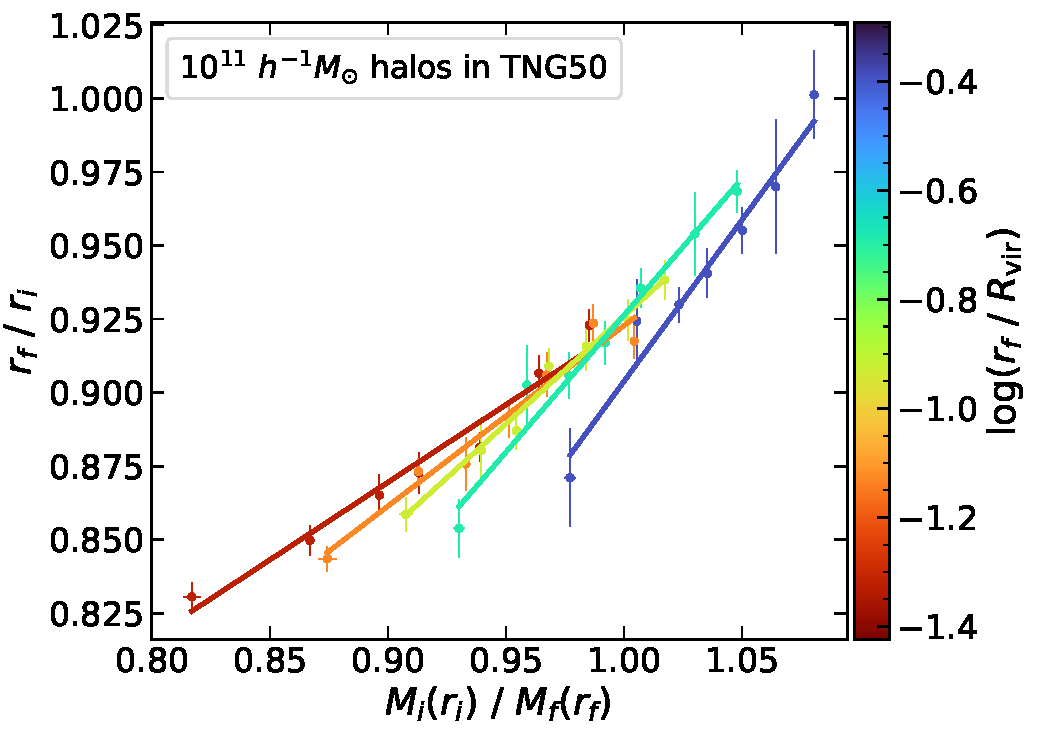
\includegraphics[width=0.48\linewidth]{plots/fit_show_rf_M_T50_M11.pdf}
    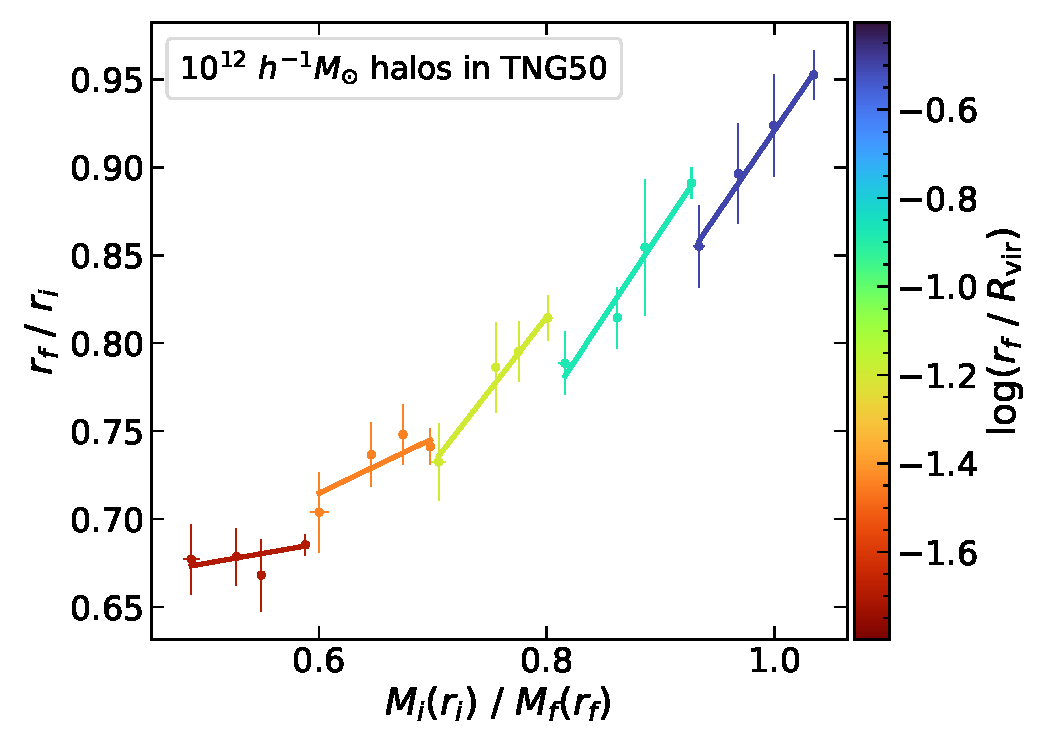
\includegraphics[width=0.48\linewidth]{plots/fit_show_rf_M_T50_M12.pdf}
    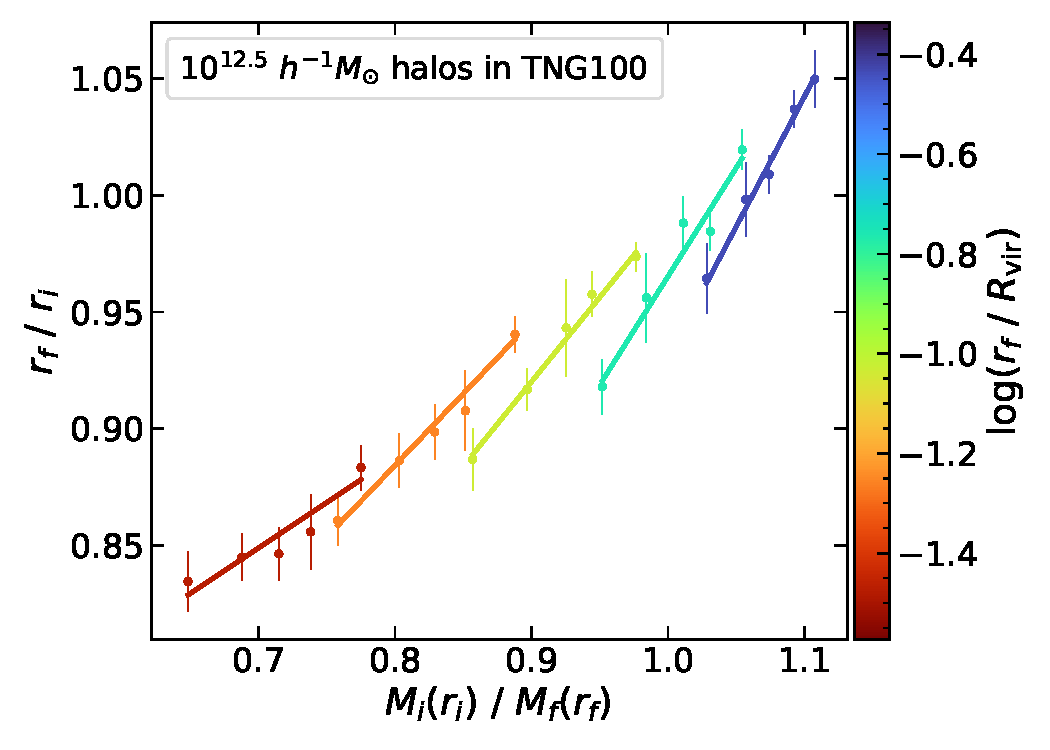
\includegraphics[width=0.48\linewidth]{plots/fit_show_rf_M_T100_M12.5.pdf}
    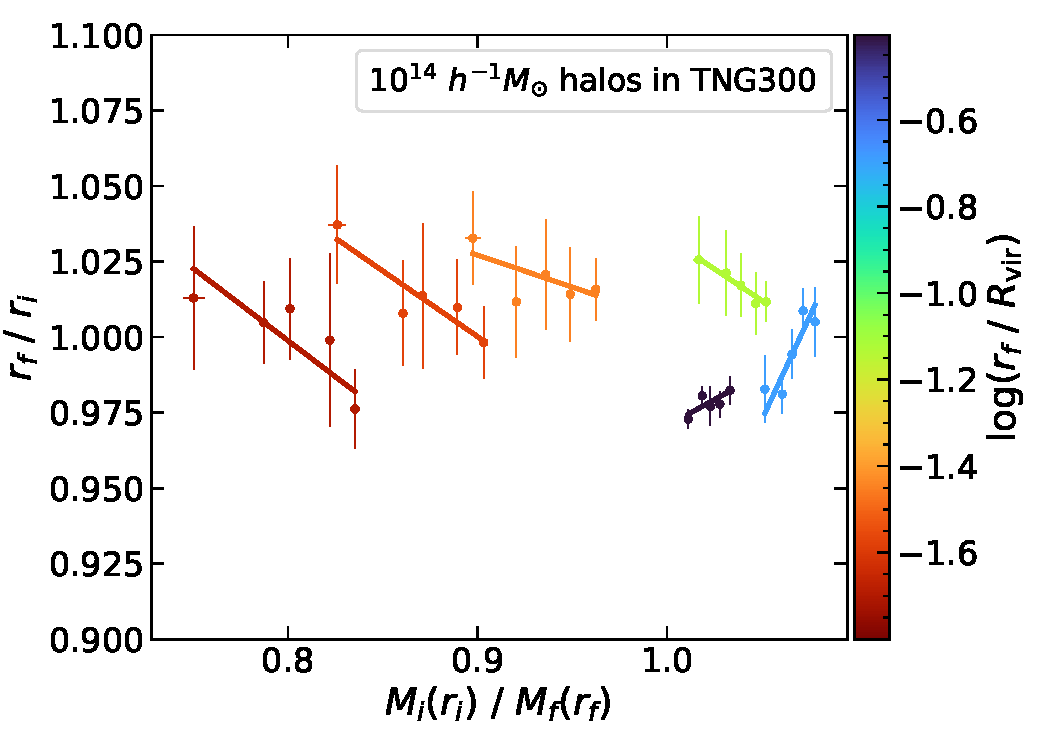
\includegraphics[width=0.48\linewidth]{plots/fit_show_rf_M_T300_M14.pdf}
    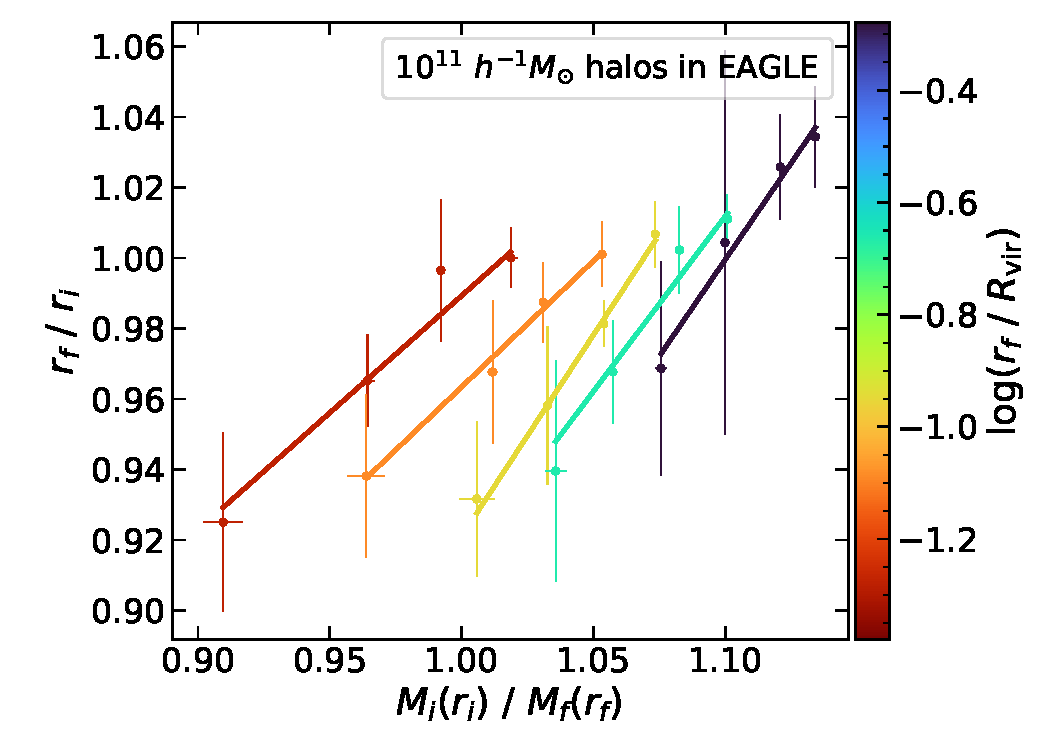
\includegraphics[width=0.48\linewidth]{plots/fit_show_rf_M_E25_M11.pdf}
    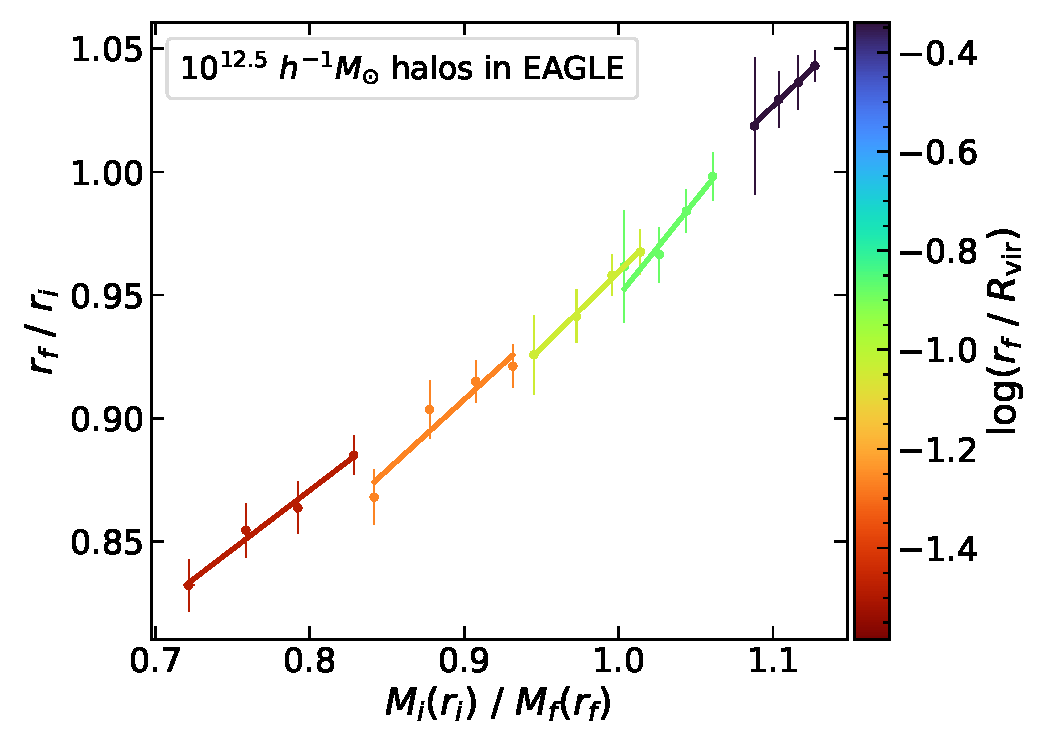
\includegraphics[width=0.48\linewidth]{plots/fit_show_rf_M_E100_M12.5.pdf}
    \caption{Relaxation relation stacked separately at 5 different radii indicated by color in six samples of haloes selected by mass from IllustrisTNG and EAGLE simulations. We also show linear polynomial fit to this relation, following \eqn{eq:chi-linear-q0-ch:z0main} with the best-fit values for the parameters $q_0$ and $q_1$ at each of the selected radii for each of the six halo samples.} %
    \label{fig:rf-fit-show-ch:z0main}
\end{figure}

In \figref{fig:rf-fit-show-ch:z0main} we show the measured relaxation relation for six different sample of haloes at shells of selected radii, compared with the best-fit model \eqn{eq:chi-linear-q0-ch:z0main} for each case; the model clearly describes these measurements extremely well. We already noted from \figref{fig:fit-view-mass-indep-ch:z0main}, that the haloes in the small volume EAGLE simulation with the reference model shows a different relaxation behaviour. This is also apparent in \figref{fig:rf-fit-show-ch:z0main}, between the $10^{11} \Mh$ haloes from that L25 simulation (last row, left panel) and the haloes of the same mass from IllustrisTNG (first row, left panel); however they both follow the linear relaxation relation at fixed radii. An interesting feature to note is the dramatic change in slope $q_1$ for the most massive haloes (middle row, right panel), with $q_1$ changing sign as one moves outwards through the halo. This also qualitatively explains the non-monotonicity and multi-valued nature of the default stacks in the lower right panel of Fig.~\ref{fig:relx-results-simple-ch:z0main}.


\begin{figure}
    \centering
    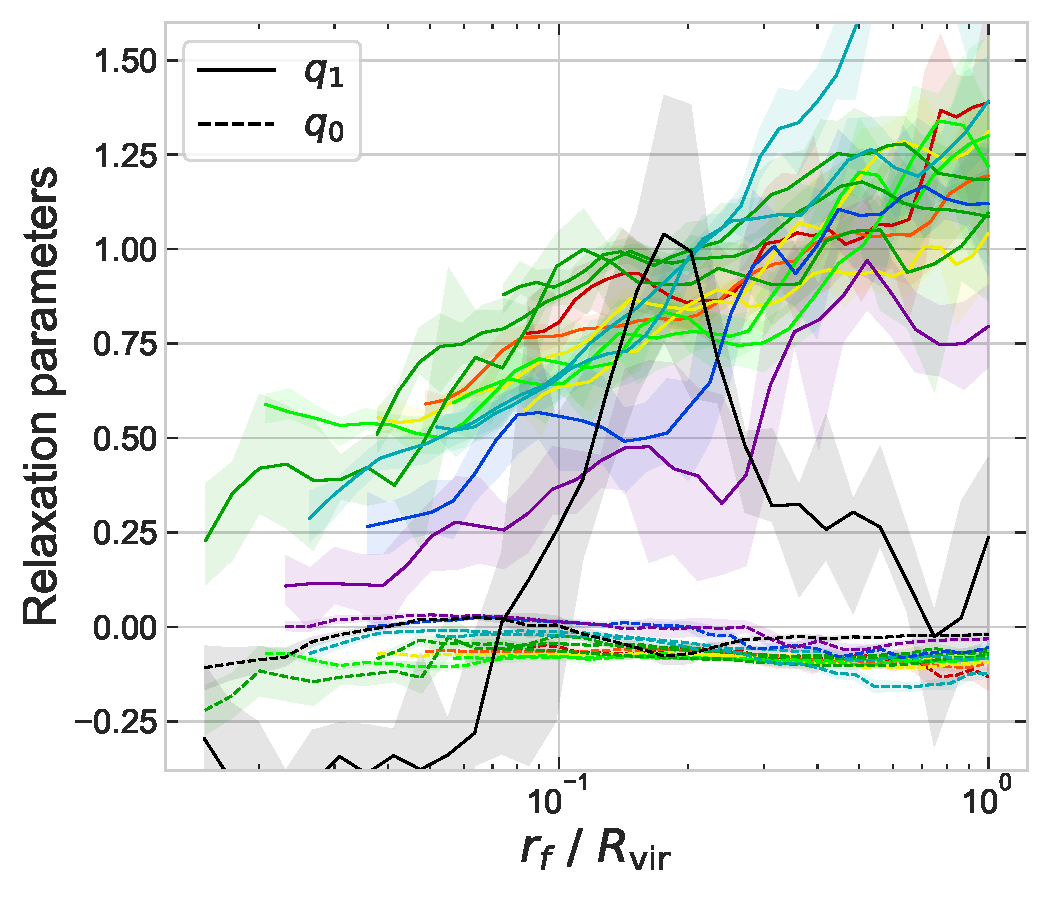
\includegraphics[width=0.49\linewidth]{plots/fit_params_rf_M_T.pdf}
    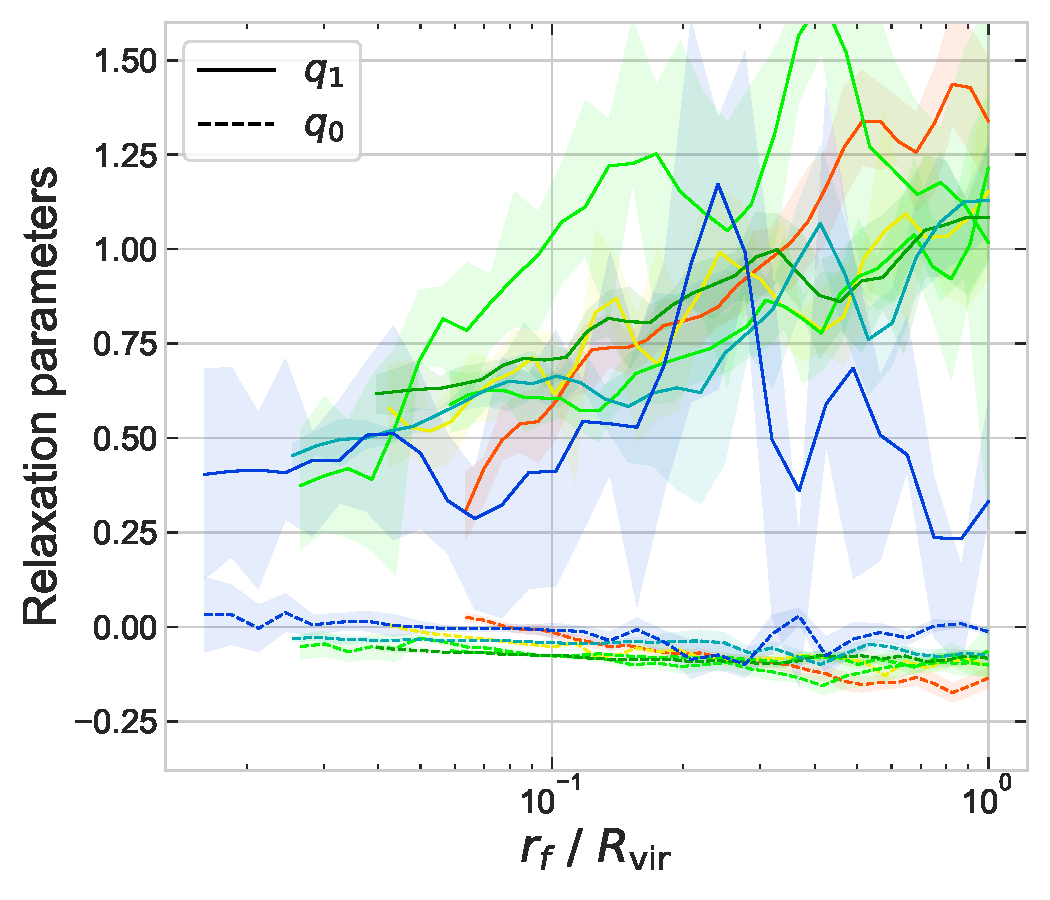
\includegraphics[width=0.49\linewidth]{plots/fit_params_rf_M_E.pdf}
    \caption{Linear quasi-adiabatic relaxation model parameters as a function of the radius of relaxed halo at different halo masses in IllustrisTNG \emph{(upper panel)} and EAGLE \emph{(lower panel)}. The colour-coding follows Fig.~\ref{fig:mass_bin_label-ch:z0main}. See text for details.}
    \label{fig:rf-fit-params-ch:z0main}
\end{figure}


\subsection{Modelling the radial dependence of the relaxation relation}
As described above, we obtained the best fit parameters $q_0$ and $q_1$ of the relaxation relation at each relaxed radius $r_f$, this is shown in \figref{fig:rf-fit-params-ch:z0main} as a function of $r_f/R_{\rm vir}$. 

For haloes of mass $M<10^{13}\Mh$, the $q_1$ parameter increases monotonically with radius and this dependence can be modelled as 
\begin{align}
q_1 (r_f) = q_{10} + q_{11} \log \left( r_f/R_{\rm vir} \right) \,,
\label{eq:q1(r_f)-ch:z0main}
\end{align}
where $q_{10}$ and $q_{11}$ are constants.
The parameter $q_0$, on the other hands, remains relatively constant at small negative values for each halo sample.
This means the factor $(1 + q_0 - q_1)$ starts with a positive value in the inner halo and becomes negative in the outer halo, inverting the relationship between change in angular momentum and mass ratio (see equation~\ref{eq:Lf-Li-ratio-ch:z0main}). And due to $q_0$ being small in magnitude, the radius at which this transition happens roughly satisfies the condition $L_f/L_i=1$. 

For cluster-scale haloes, this simple monotonic dependence of $q_1(r_f)$ is replaced with oscillatory behaviour. In fact, some of the peaks in $q_1$ correspond to $q_1\approx1$; combined with $|q_0|\ll1$, this indicates that these peaks are shells which nearly perfectly conserve angular momentum. (E.g., this happens at $r_f/R_{\rm vir}\simeq0.5\,(0.2)$ for $M=10^{13.5}\,(10^{14})\Mh$.)
This is in strong contrast to \figref{fig:fit-view-mass-indep-ch:z0main} where the slope of the relaxation relation represented by a globally defined $q_1$ (e.g., equation~\ref{eq:chi-linear-q0-ch:z0main} without explicit $r_f$ dependence in the parameters) is close to zero for these haloes, indicating maximum deviation from the adiabatic relaxation. This complicated behaviour in the cluster-scale haloes could be due to the presence of substructures. The $q_0$ parameter now also shows interesting behaviour; it is only slightly negative in the outer halo but becomes close to zero in the inner halo for these haloes ($q_0$ was relatively constant with more negative value for less massive haloes).
 

Excluding those cluster scale haloes, we propose a three parameter model as an extension to the quasi-adiabatic relaxation model, where the relaxation ratio depends linearly on the mass ratio as in \eqn{eq:chi-linear-q0-ch:z0main}, however the slope of this relationship has explicit logarithmic dependence on the radius:
\begin{align}
\label{eq:q3-model-ch:z0main}
\frac{r_f}{r_i} - 1 &=  \left[ q_{10} + q_{11} \log \left( \frac{r_f}{R_{\rm vir}} \right) \right] \left( \frac{M_i(r_i)}{M_f(r_f)} - 1 \right) + q_0
\end{align}
Using this model we can quantify the response of these haloes to galaxy formation;
in \figref{fig:3-param-mass-only-ch:z0main}, we show these 3 parameters estimated as a function of halo mass for IllustrisTNG and EAGLE. We see that each of the parameters is nearly mass-independent for $M\lesssim10^{12}\Mh$, showing significant trends with mass only above $M\gtrsim10^{12.5}\Mh$ (with the exception of $10^{10.5} \Mh$ in EAGLE). This simplified but accurate relaxation model can be of great use in modelling the rotation curves of low-mass and Milky Way-like galaxies \citep{2021MNRAS.503.4147P,2021MNRAS.507..632P}, which we will explore in future work.

\begin{figure}
    \centering
    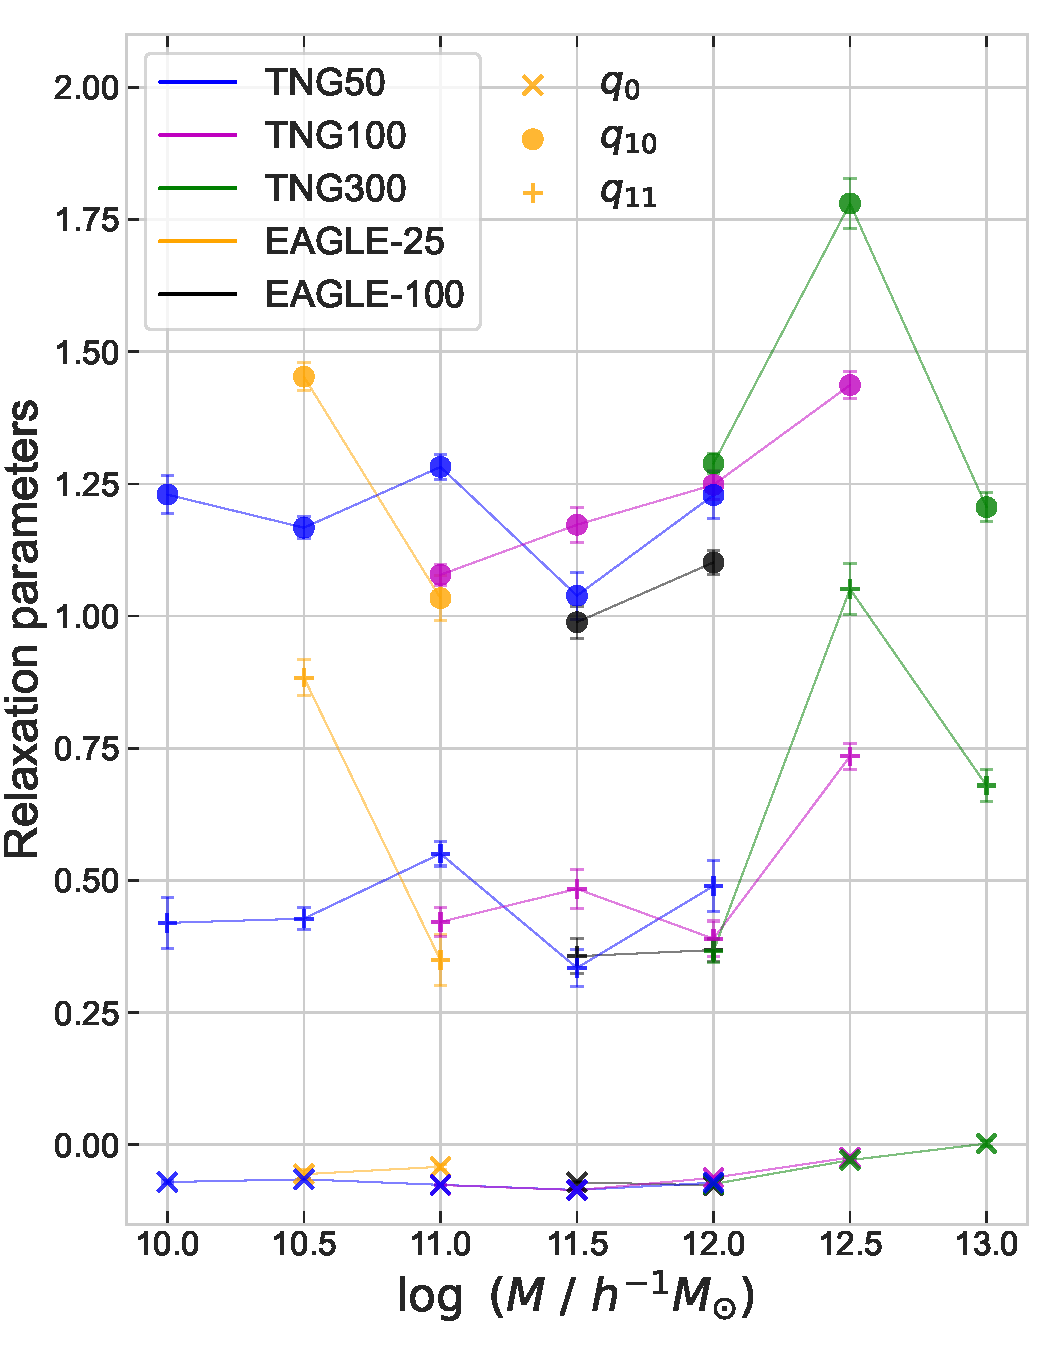
\includegraphics[width=.7\linewidth]{plots/fit_param_q3s_M_TE.pdf}
    \caption{Fitting values for the three parameters namely $q_{0}$, $q_{10}$ and $q_{11}$ in radially dependent quasi-adiabatic relaxation model described by equation~\ref{eq:q3-model-ch:z0main} as a function of halo mass in the three IllustrisTNG simulations and the two EAGLE simulations.}
    \label{fig:3-param-mass-only-ch:z0main}
\end{figure}


\section{Properties beyond halo mass}
\label{sec:dep-on-hal-gal-props-ch:z0main}
In this section, we study our parametrised model of the response of dark matter in the halo as a function of halo and galaxy properties beyond halo mass. This is motivated by the fact that there is a significant scatter in the relaxation relation (see Fig.~\ref{fig:relx-results-simple-ch:z0main}), even within halo samples selected by mass. Such a study would also have implications for halo assembly bias and similar environmental correlations predicted in the $\Lambda$CDM framework  \citep[see, e.g., the discussion in][]{2021arXiv211200026P}. 


For the simulations from TNG suite, we focus on the following halo properties in addition to their mass. For the haloes in the gravity-only runs, we define the concentration as $c=2.1626 \times R_{\rm vir}/R_{V_{\rm{max}}}$, where $R_{V_{\rm{max}}}$ is the radius at which the rotation curve attains its peak. If the sphericalised mass profile of these haloes had a perfectly NFW form, this concentration would be exactly equal to the standard NFW concentration defined in terms of NFW scale radius \citep[see equation 5 of ][]{1996ApJ...462..563N}. 
This definition of concentration is convenient since it does not require any statistical fit to the measured halo profile.
For the haloes in hydrodynamic simulations, we consider 
three different properties, namely, \textbf{gas fraction} $(f_g)$ of the whole FOF group, and the \textbf{stellar mass fraction} $(f_{\ast})$ and specific star formation rate \textbf{(SSFR)} of the central subhalo associated to each of them. 
\begin{align}
    f_{g} = \frac{M_{g}^{\rm{F}}}{M^{\rm{F}}}\,; \quad
    f_{\ast} = \frac{M_{\ast}^{\rm{S}}}{M^{\rm{S}}}\,; \quad {\rm SSFR} = \frac{\rm{SFR}}{M_{\ast}^{\rm{S}}}\,.
\label{eq:galpropdefs-ch:z0main}
\end{align}
Here $M^{\rm{F}}$ ($M_{g}^{\rm{F}}$) denotes the total mass of all (gas) particles in the FOF group, whereas $M^{\rm{S}}$ ($M_{\ast}^{\rm{S}}$) denotes the total mass of all (stellar) particles in the associated central subhalo. 
Finally, SFR denotes the sum of star formation rate of all gas cells in the central subhalo. The above definitions allow us to track the response of dark matter to the gas content of the full halo and the stellar content and activity of its central galaxy. We have also checked that using the stellar content and activity of the full halo leads to qualitatively similar results as when using the central galaxy alone. All these four halo/galaxy properties show overall trend with halo mass, however, there is also a considerable scatter even at fixed mass scale, this is illustrated in \figref{fig:halo-prop-pers-data-ch:z0main}. 

\begin{figure}[htbp]
    \centering
    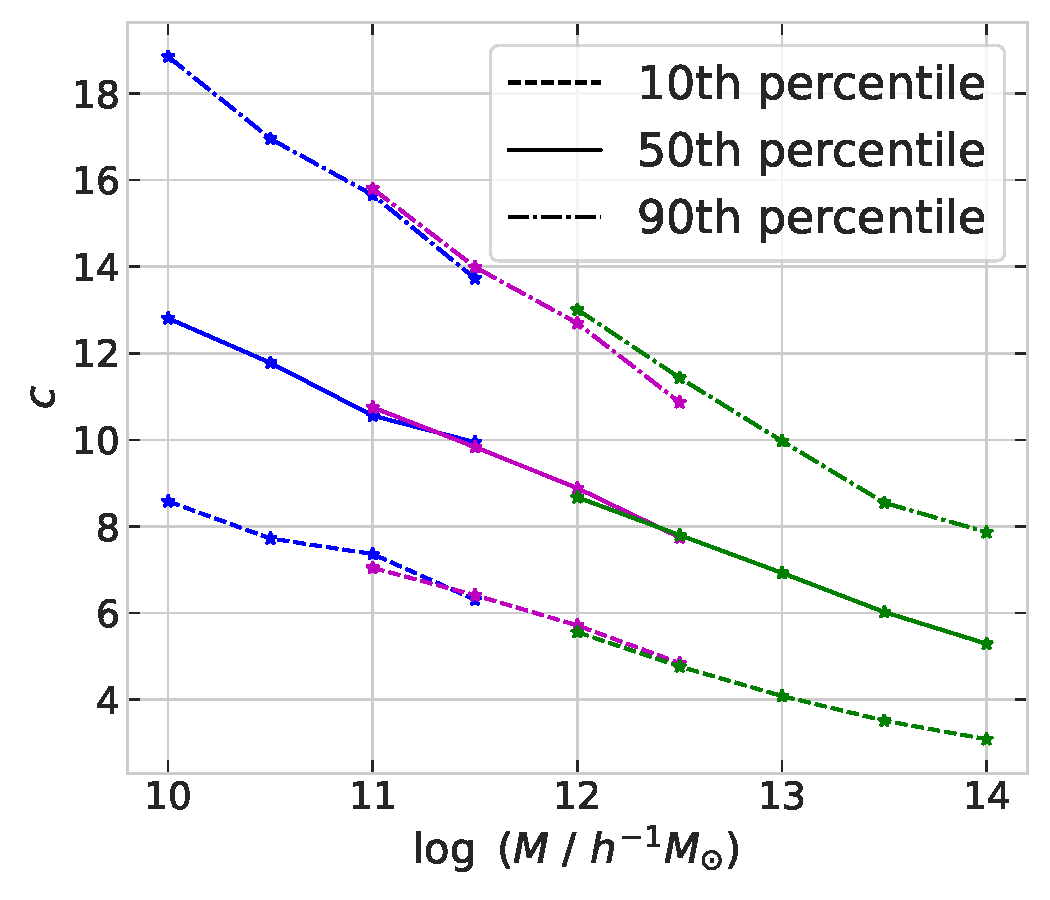
\includegraphics[clip,trim={0.2cm 1.18cm 0.25cm 0.3cm},width=0.4\linewidth]{plots/percentile_data_M-cs_T.pdf}
    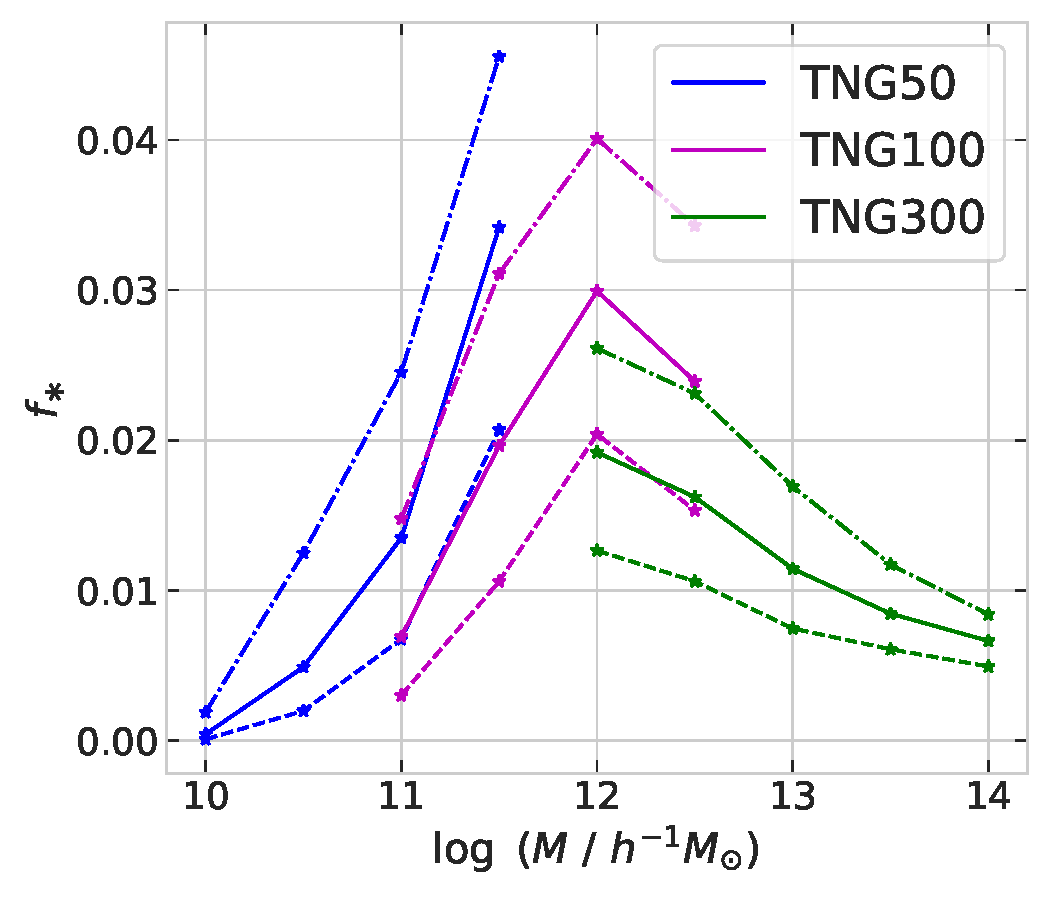
\includegraphics[clip,trim={0.2cm 1.18cm 0.25cm 0.3cm},width=0.4\linewidth]{plots/percentile_data_M-fs1_T.pdf}
    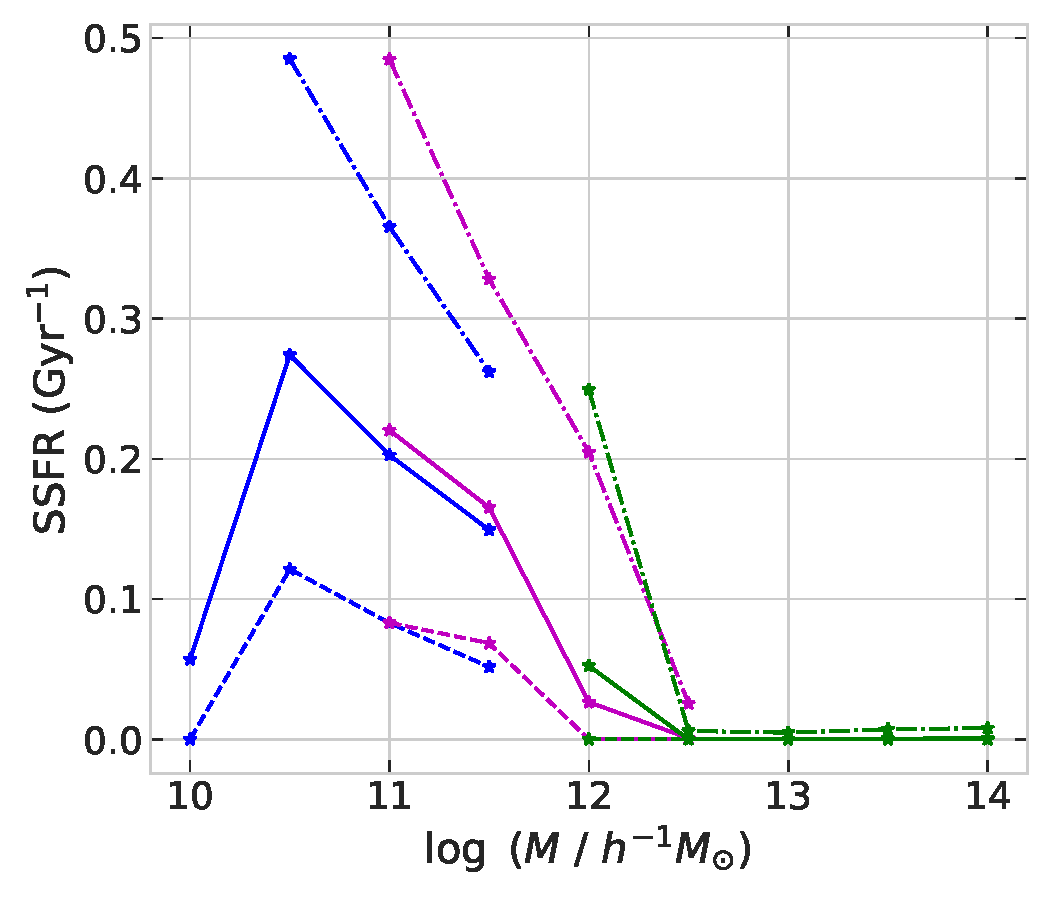
\includegraphics[clip,trim={0.2cm 0cm 0.25cm 0.3cm},width=0.4\linewidth]{plots/percentile_data_M-ssfr1_T.pdf}
    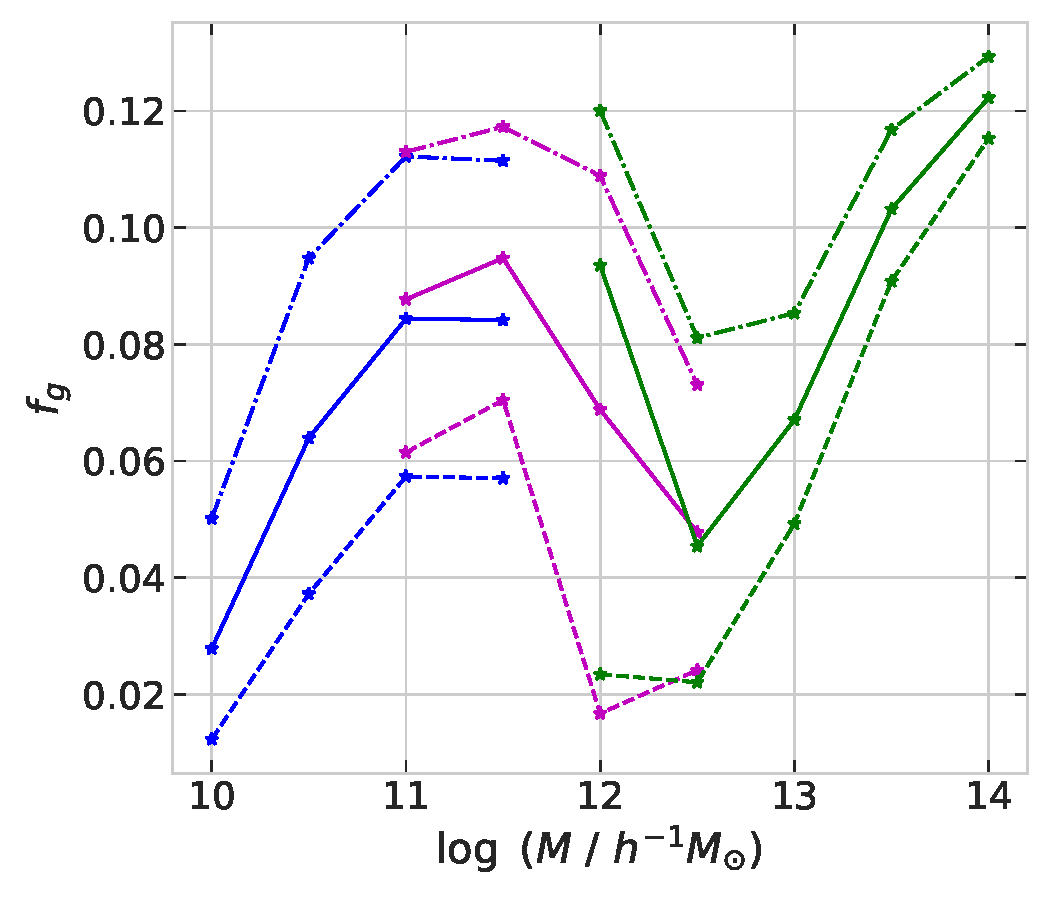
\includegraphics[clip,trim={0.2cm 0cm 0.25cm 0.3cm},width=0.4\linewidth]{plots/percentile_data_M-fg_T.pdf}
    \caption{The 10th, 50th and 90th percentile of the four different halo properties in each of the sample selected by mass from three different cosmological boxes of the IllustrisTNG.
    This includes the concentration ($c$) of the unrelaxed halo, and the stellar fraction ($f^{\ast}$), specific star formation rate (SSFR) and gas fraction ($f_g$) of the hydrodynamical halo, all of which are defined in main text.} %
    \label{fig:halo-prop-pers-data-ch:z0main}
\end{figure}

For all subsamples selected by a secondary halo/galaxy property at fixed halo mass, we use the 3-parameter model discussed above in the mass range $10^{10}$ to $10^{12.5}$ $\Mh$, 
while for cluster-scale haloes, where our 3-parameter model fails, we directly compare the linear quasi-adiabatic relaxation model parameters $q_0$ and $q_1$ as a function of the scaled halo-centric radius $r_f/R_{\rm vir}$. The results for low-mass (massive) haloes are shown in Fig.~\ref{fig:fit-fit-func-q-ch:z0main} (Fig.~\ref{fig:fit-func-rf-13514-ch:z0main}).


For reference, the upper panels of Fig.~\ref{fig:fit-fit-func-q-ch:z0main} show the best-fit values of $q_0$, $q_{10}$ and $q_{11}$ as a function of halo mass alone for haloes with $M\leq10^{13}\Mh$,
which repeat the corresponding curves in Fig.~\ref{fig:3-param-mass-only-ch:z0main}. The upper panels of Fig.~\ref{fig:fit-func-rf-13514-ch:z0main} similarly repeat the results for $q_0(r_f)$ and $q_1(r_f)$ for the mass bins $M=10^{13},10^{13.5},10^{14}\Mh$ from Fig.~\ref{fig:rf-fit-params-ch:z0main}. By displaying both, the full radial dependence as well as the 3-parameter description for the mass bin $10^{13}\Mh$, we can assess the reliability of the latter around the mass scale where it begins to fail. We repeat this for subsamples split by secondary halo/galaxy properties below.



\subsection{Dependence on unrelaxed halo concentration}
Unrelaxed haloes at fixed mass, as found in gravity-only simulations are known to have universal mass profiles characterised by their concentration, together with their mass.
As can already be noted in \figref{fig:halo-prop-pers-data-ch:z0main}, this NFW concentration is correlated with the halo mass \citep[see e.g. ][]{2006ApJ...652...71W,2007MNRAS.378...55M,2015ApJ...799..108D,2017MNRAS.468.2984P}.
In order to isolate the effect of concentration on the response, we define \textbf{concentration significance} $(c_s)$.
\begin{align}
c_s = \left(\log c- \log \bar{c}(M)\right)/\sigma\,. \nonumber
\end{align}
Here we use the median $\bar{c}(M)$ and scatter $\sigma$ of the concentration-mass relation as given by Diemer et al. (2019) \citep{2019ApJ...871..168D} and computed with the COLOSSUS code \citep[][]{2018ApJS..239...35D}.

Then we select haloes from each of the mass bins in three separated $c_s$ percentile bins $(10\pm10, ~50\pm10 ~\&~ 90\pm10)$  and compute the relaxation relation as described in previous sections for each of those samples. 
We find that $q_0$ shows strong dependence on the concentration, with more concentrated haloes having higher value of $q_0$ at most halo masses with $M \leq 10^{13} \Mh$ (see second row in \figref{fig:fit-fit-func-q-ch:z0main} and second row, first column in \figref{fig:fit-func-rf-13514-ch:z0main}). This can be understood in terms of the formation time of the halo, since concentration is correlated with the formation time. More concentrated haloes, that have formed earlier might have had enough time for the dark matter to respond to the baryonic feedback, and hence there is less offset. On the other hand, $q_{10}$ or $q_{11}$ display a more complex dependence at low mass, with no clear monotonic trend. Meanwhile, for cluster-scale haloes, $q_1$ shows a very different behaviour as a function of $r_f$ at different halo concentrations (see second row of \figref{fig:fit-func-rf-13514-ch:z0main}). We leave a fuller exploration of these trends, particularly their dependence on substructure properties, to future work.



\begin{figure}
    \centering
    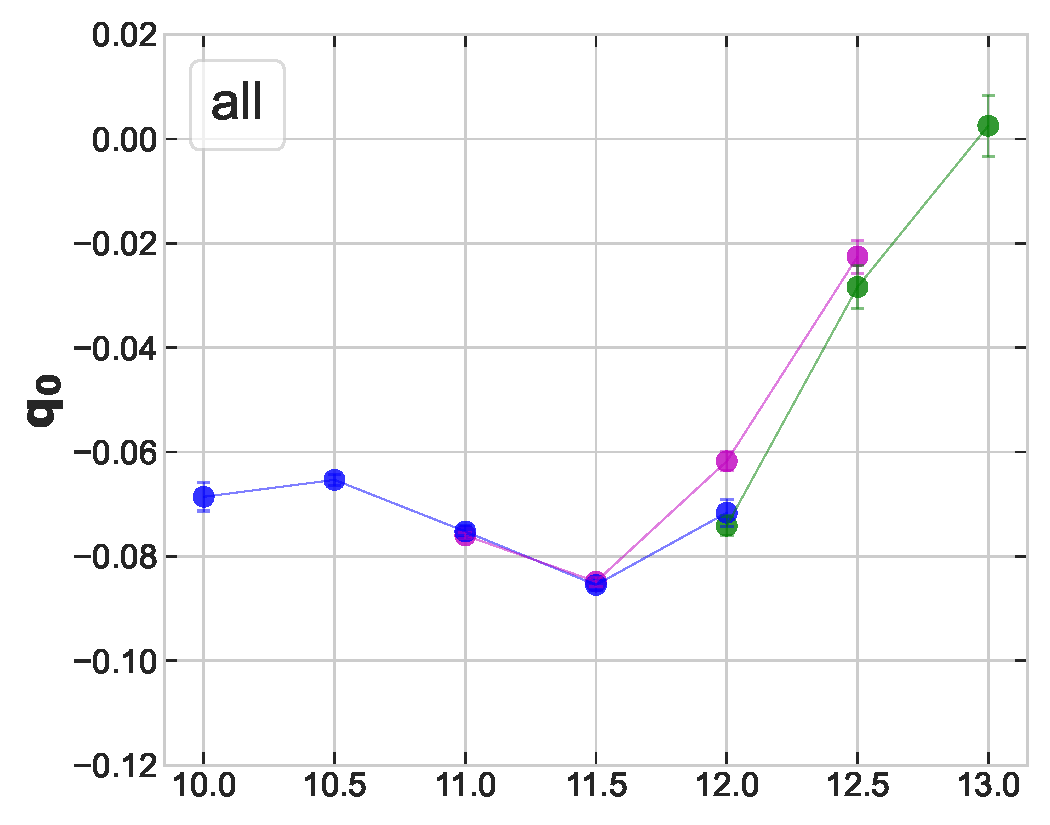
\includegraphics[width=0.32\linewidth]{plots/fit_param_q0_M_T.pdf}
    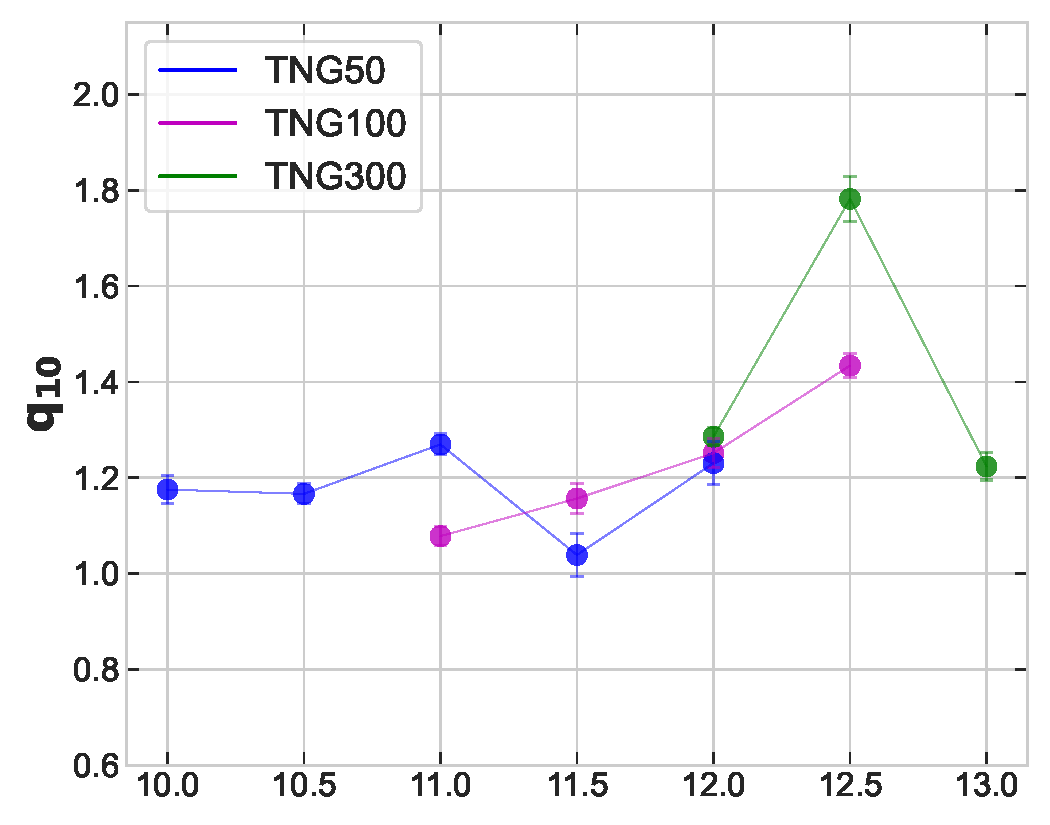
\includegraphics[width=0.32\linewidth]{plots/fit_param_q10_M_T.pdf}
    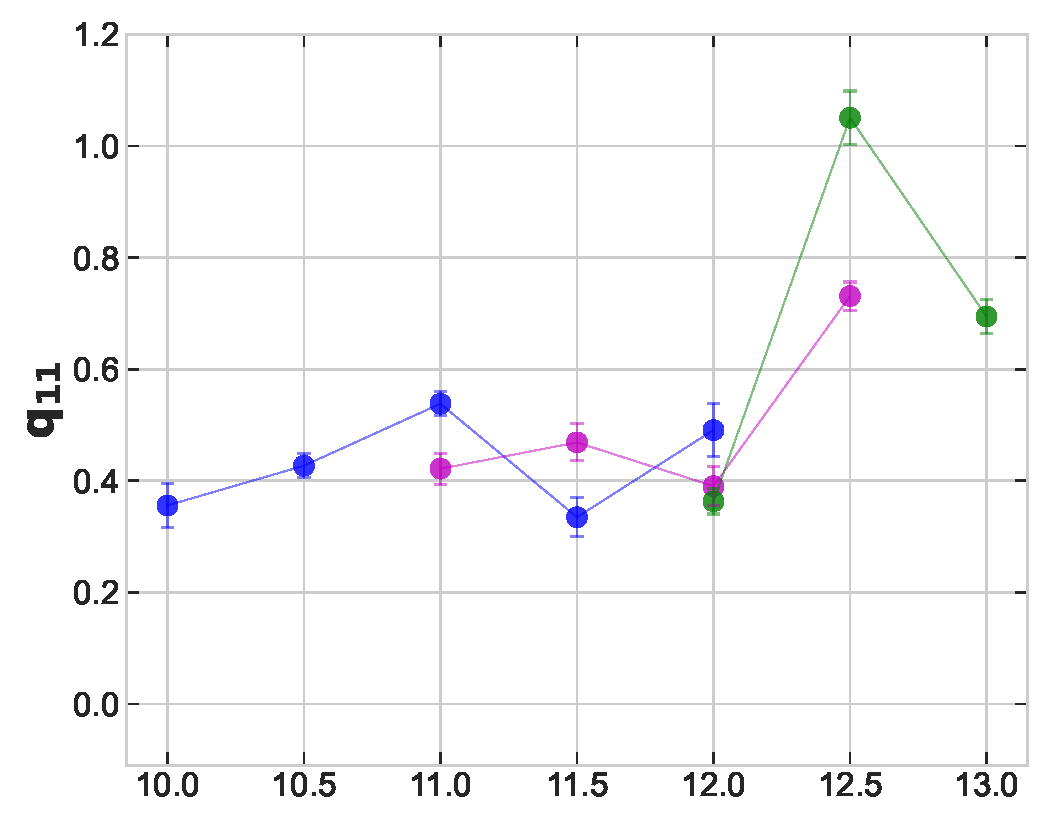
\includegraphics[width=0.32\linewidth]{plots/fit_param_q11_M_T.pdf}
    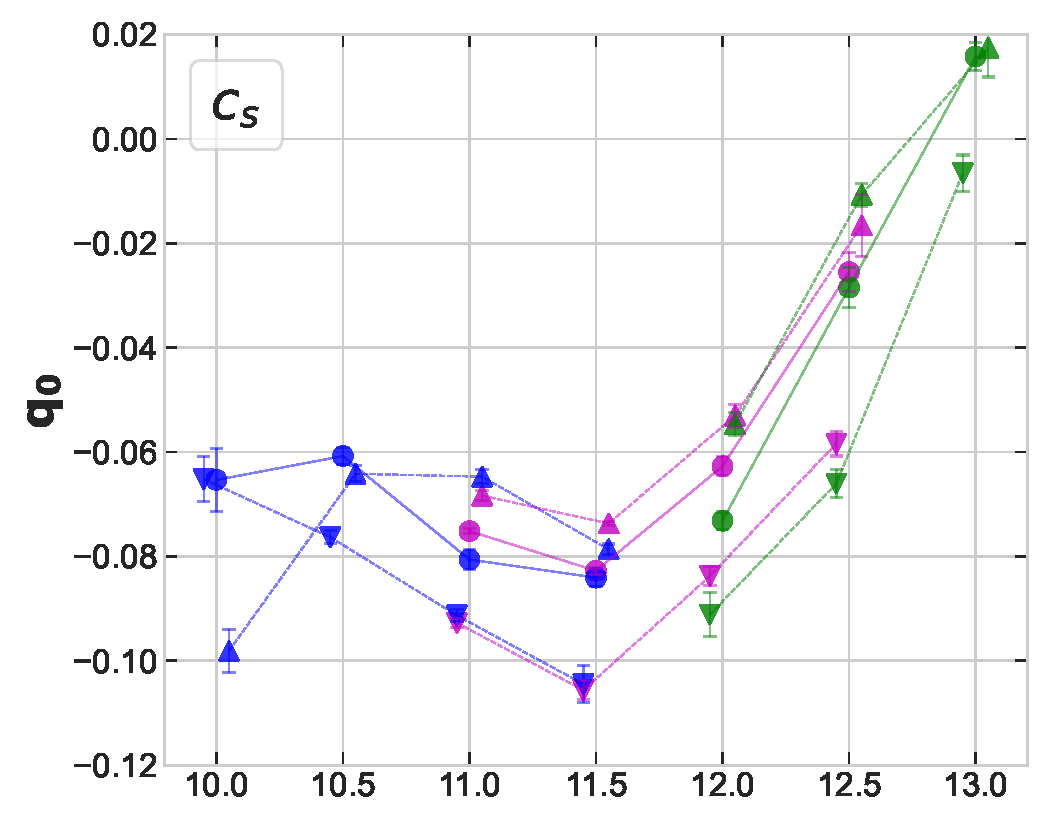
\includegraphics[width=0.32\linewidth]{plots/fit_param_q0_M-cs_T.pdf}
    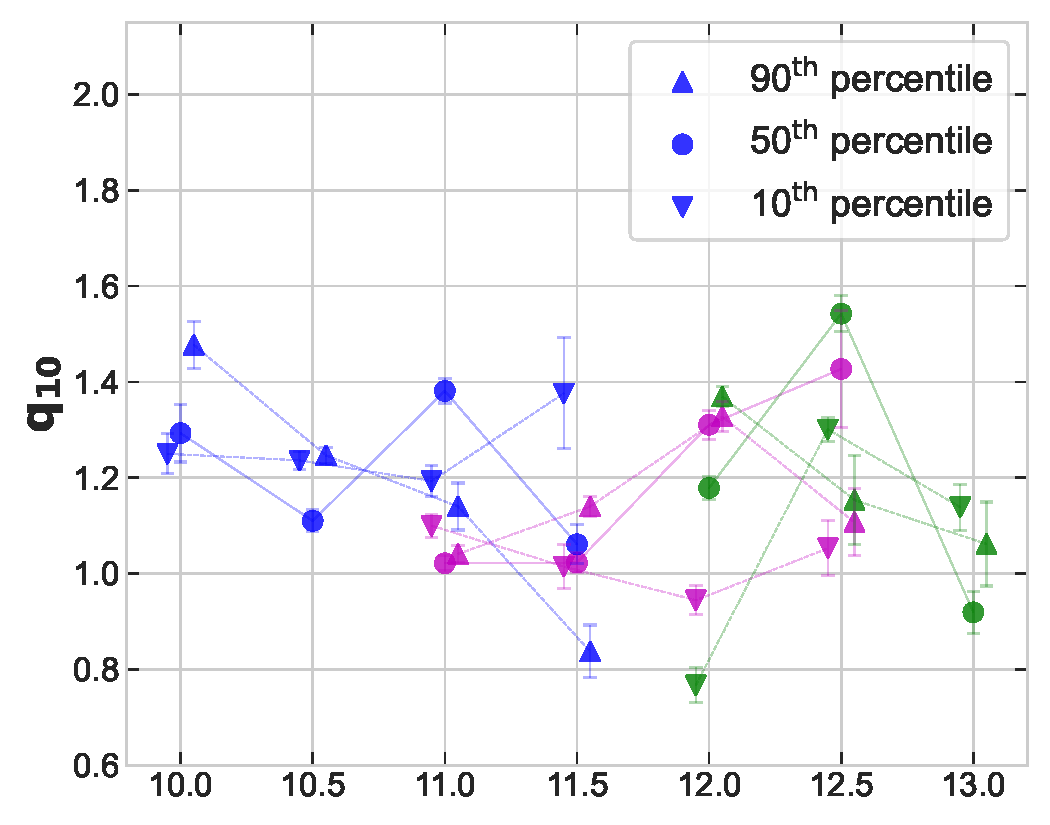
\includegraphics[width=0.32\linewidth]{plots/fit_param_q10_M-cs_T.pdf}
    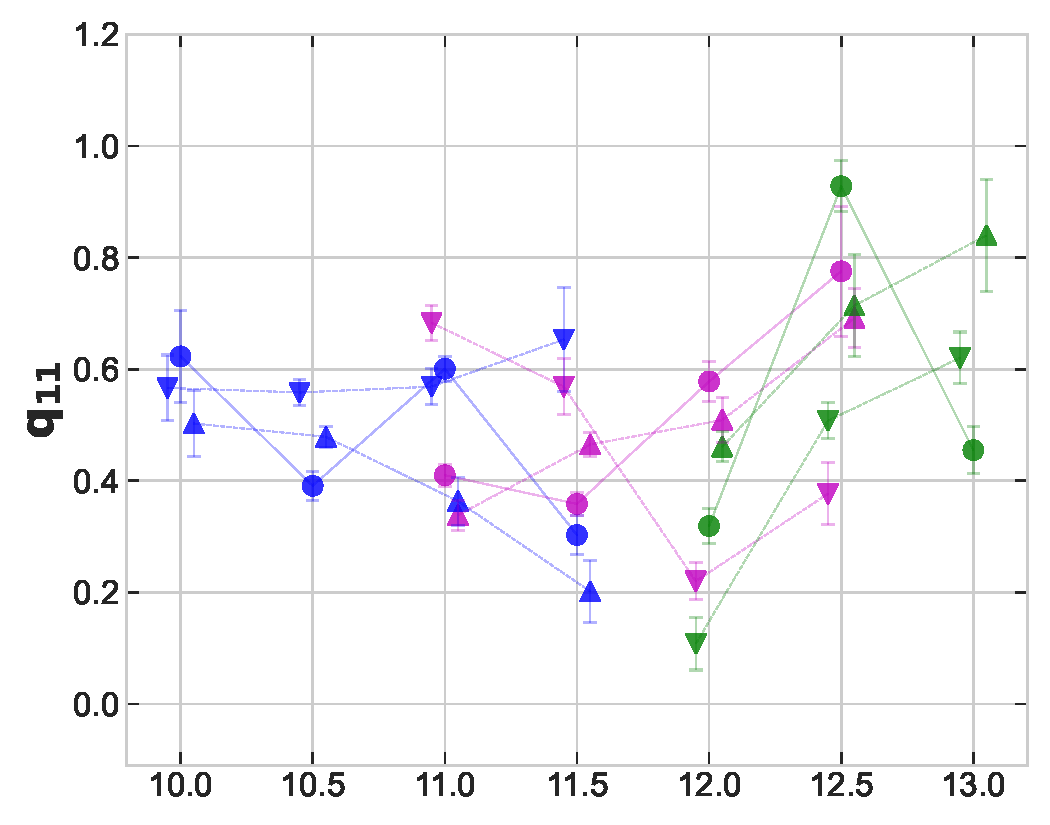
\includegraphics[width=0.32\linewidth]{plots/fit_param_q11_M-cs_T.pdf}
    
    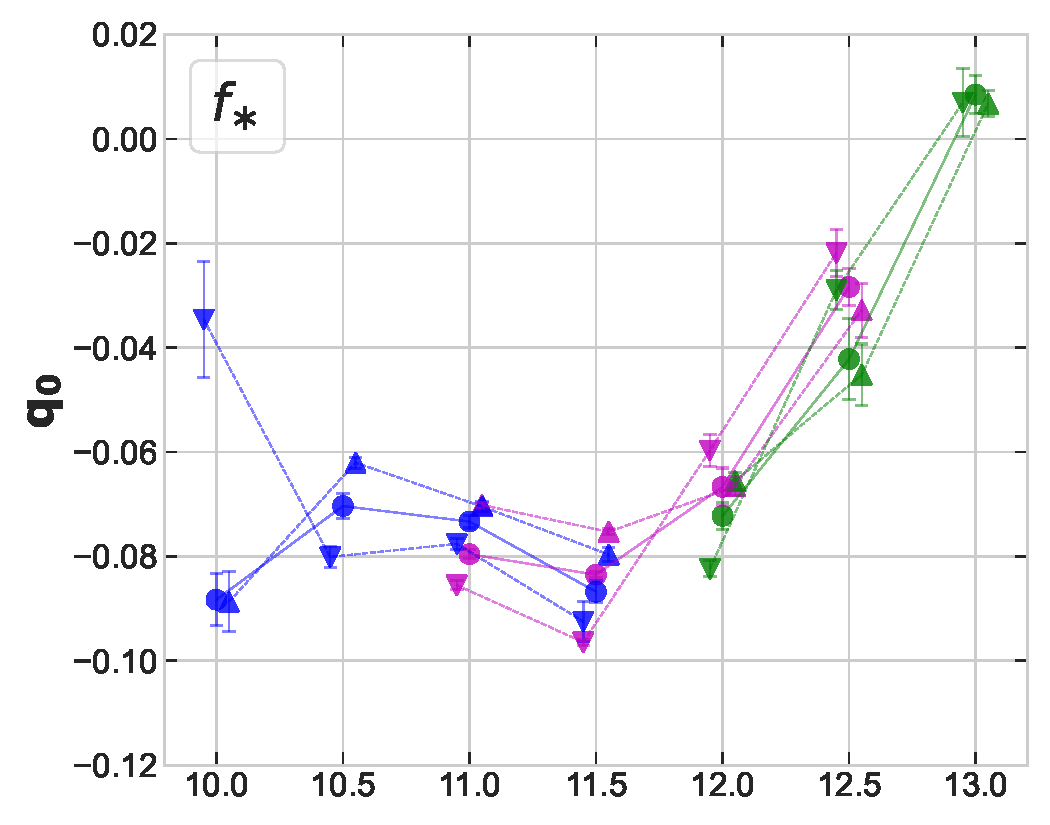
\includegraphics[width=0.32\linewidth]{plots/fit_param_q0_M-fs1_T.pdf}
    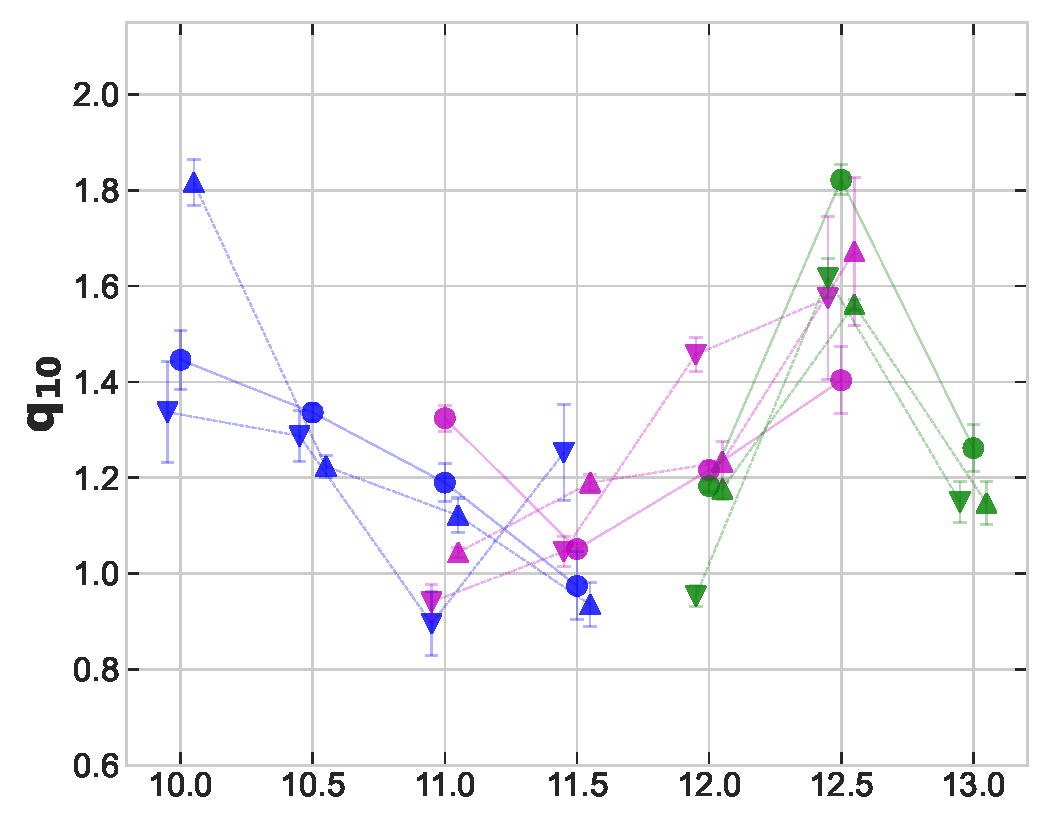
\includegraphics[width=0.32\linewidth]{plots/fit_param_q10_M-fs1_T.pdf}
    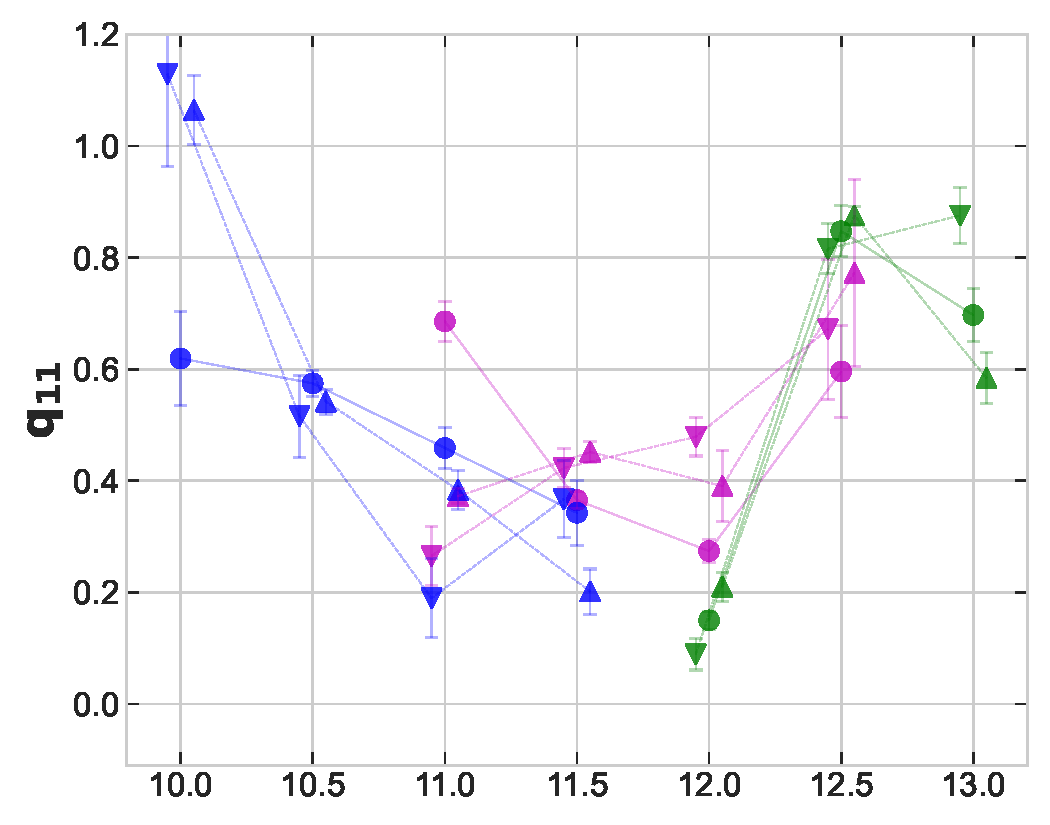
\includegraphics[width=0.32\linewidth]{plots/fit_param_q11_M-fs1_T.pdf}
    
    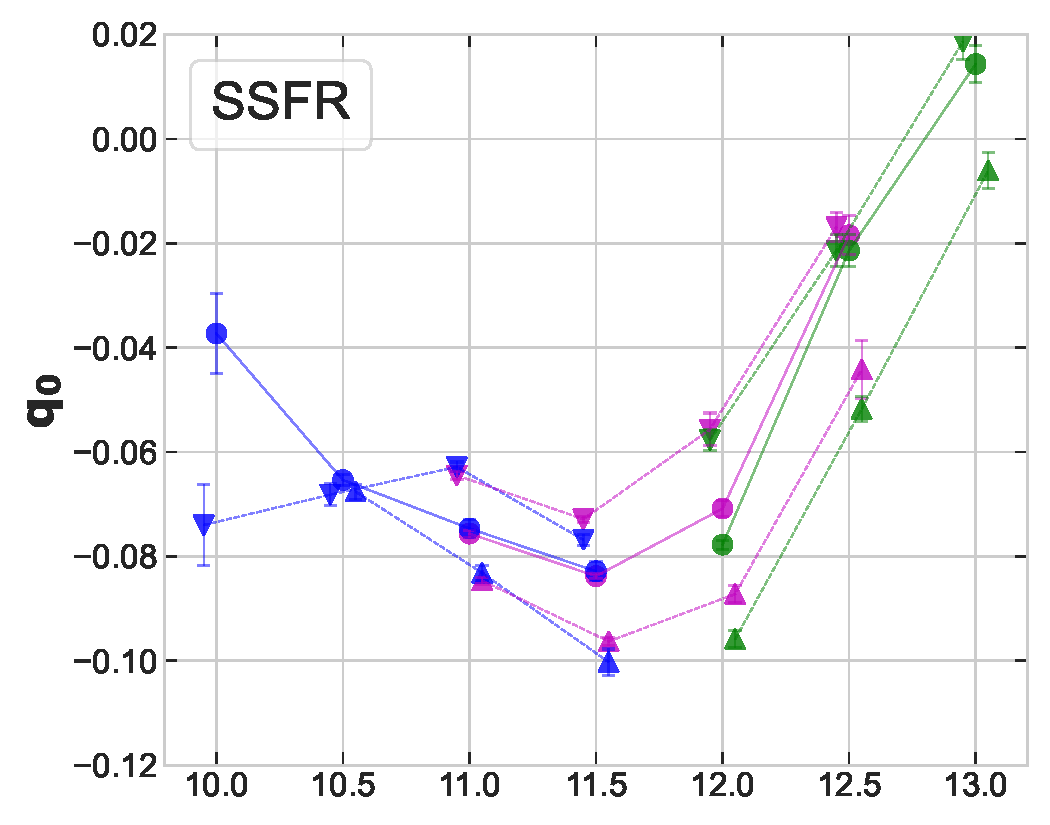
\includegraphics[width=0.32\linewidth]{plots/fit_param_q0_M-ssfr1_T.pdf}
    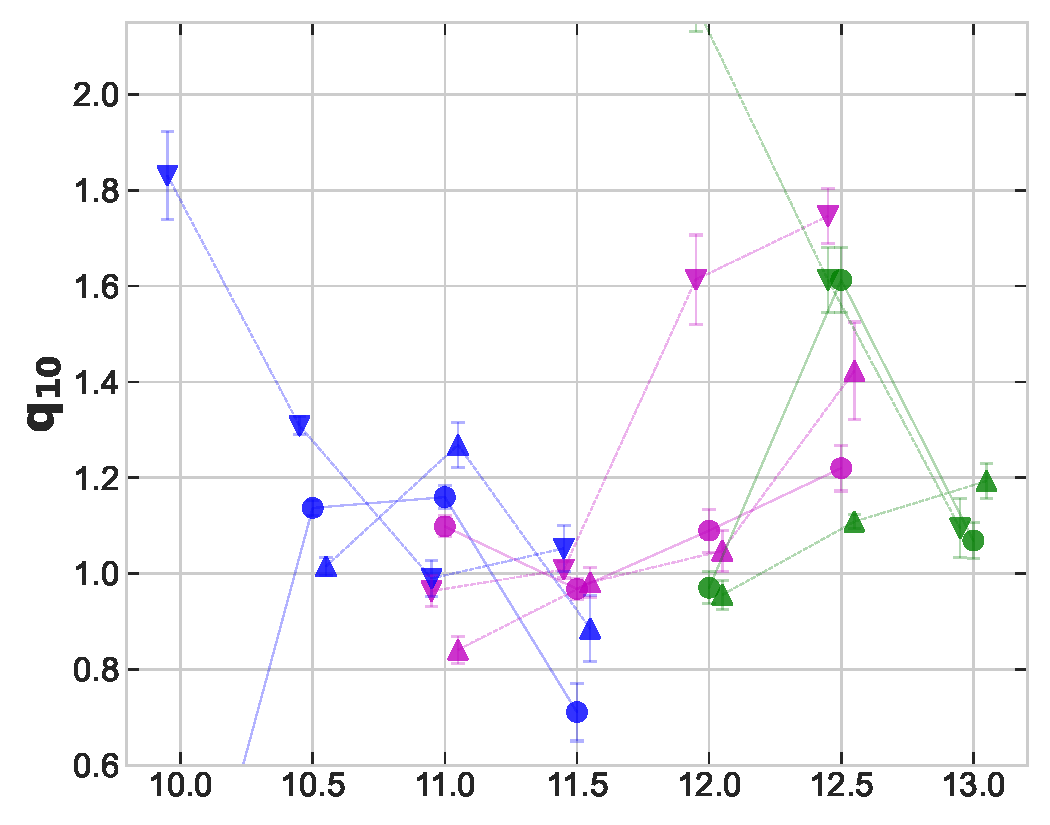
\includegraphics[width=0.32\linewidth]{plots/fit_param_q10_M-ssfr1_T.pdf}
    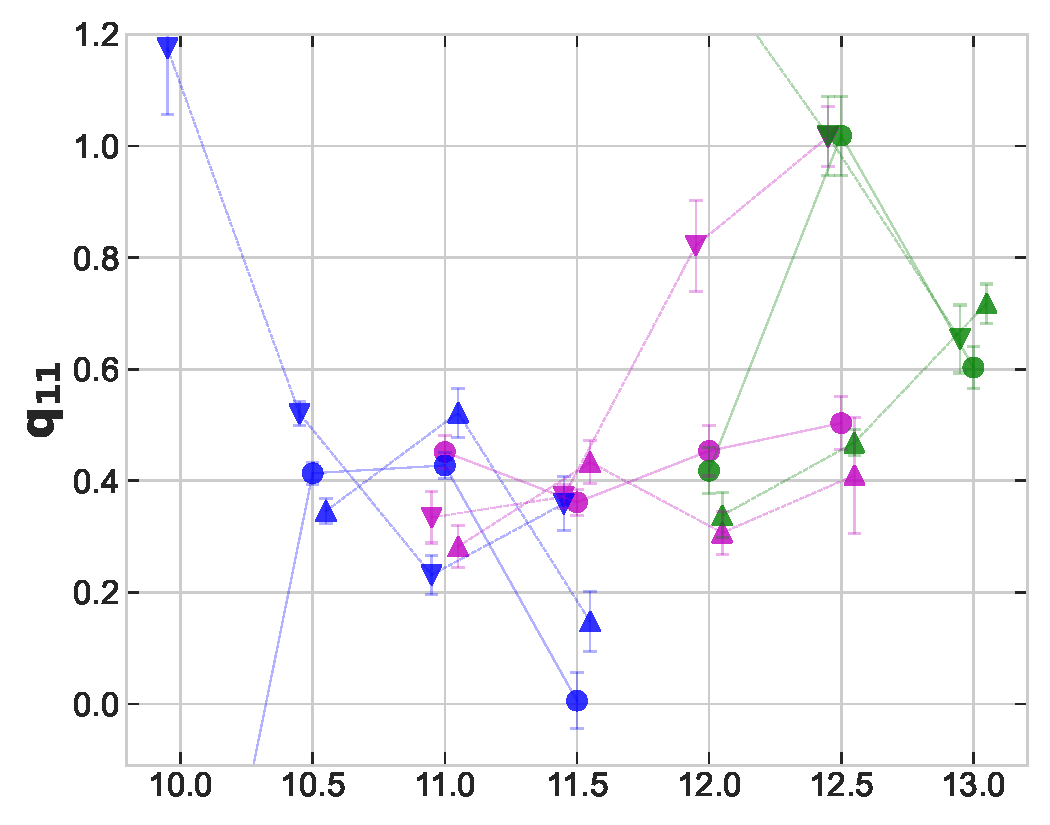
\includegraphics[width=0.32\linewidth]{plots/fit_param_q11_M-ssfr1_T.pdf}
    
    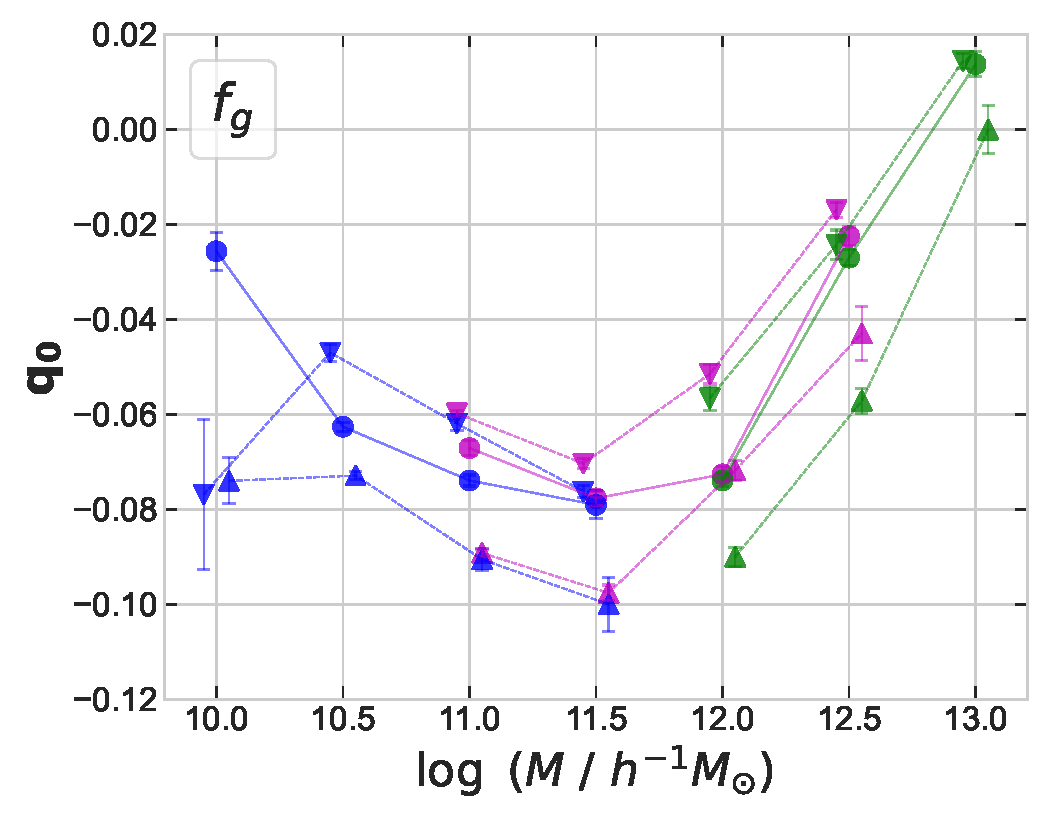
\includegraphics[width=0.32\linewidth]{plots/fit_param_q0_M-fg_T.pdf}
    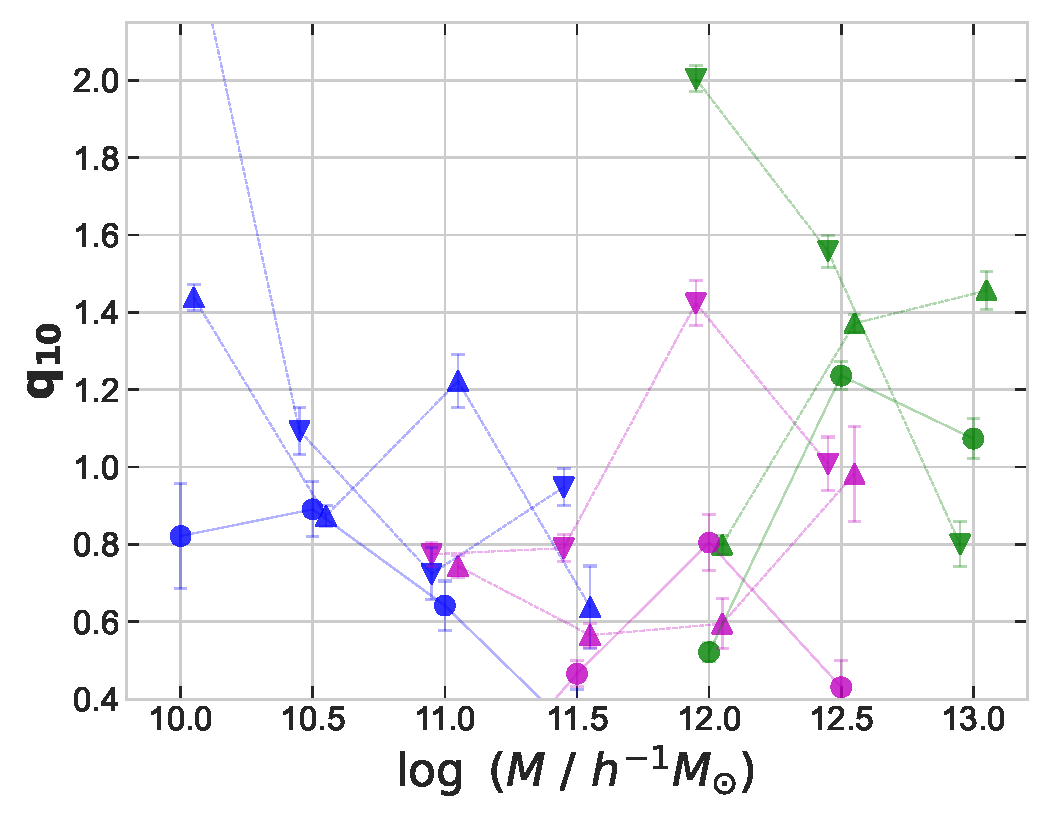
\includegraphics[width=0.32\linewidth]{plots/fit_param_q10_M-fg_T.pdf}
    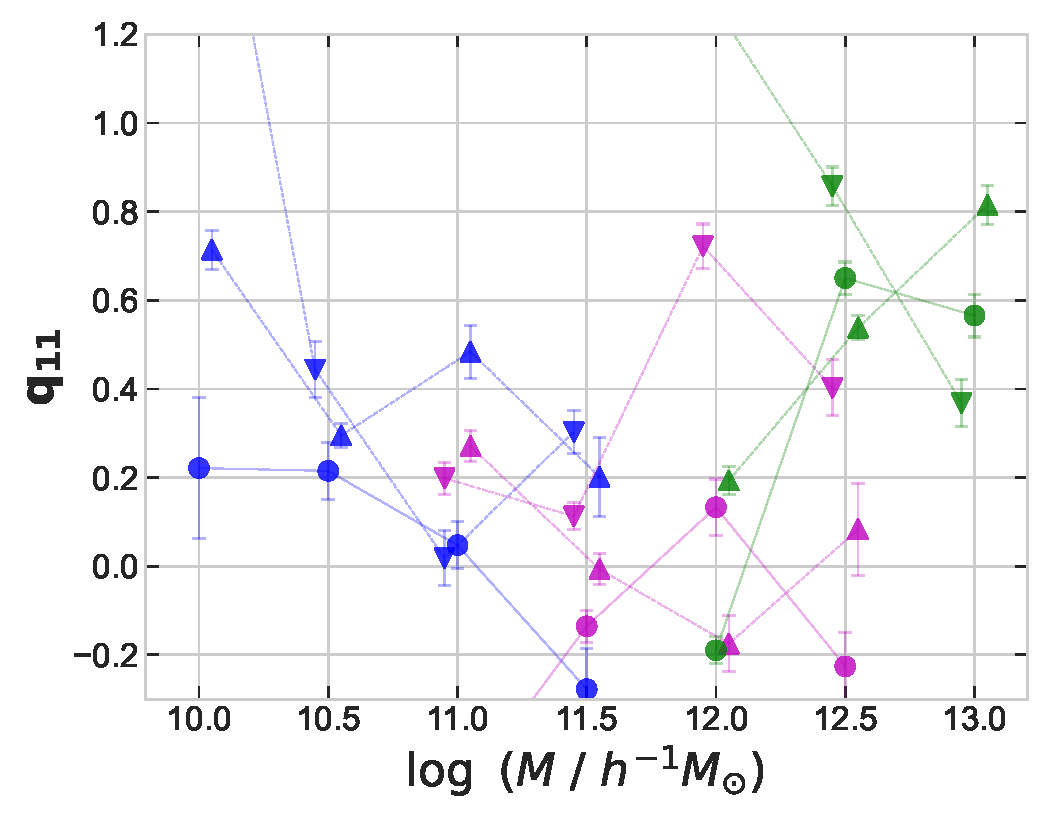
\includegraphics[width=0.32\linewidth]{plots/fit_param_q11_M-fg_T.pdf}
    \caption{Radially dependent quasi-adiabatic relaxation model parameters $q_{0}$, $q_{10}$ and $q_{11}$ estimated as a function of halo properties in IllustrisTNG simulations. In the top row panels, only halo mass dependence is shown; whereas in the next three rows, we show the dependence on halo concentration, stellar mass fraction, specific star formation rate and gas fraction in terms of percentiles respectively.} %
    \label{fig:fit-fit-func-q-ch:z0main}
\end{figure}


\subsection{Dependence on baryonic halo properties}
We now shift our focus to hydrodynamical halo properties. In this regard, we study the response as a function of the three halo properties defined above; namely the specific star formation rate (SSFR) at current redshift $z=0$ and the total stellar mass fraction ($f_{\ast}$) and gas fraction ($f_g$) at redshift $z=0$ which respectively represent the integrated star formation activity and gas content of the central subhalo. At each halo mass bin, we take three subsamples selected by bins of percentiles in $f_{\ast}$, SSFR and $f_g$, in a similar fashion as with concentration significance. %

From the third column of \figref{fig:fit-fit-func-q-ch:z0main}, we note that $f_\ast$ does not affect the relaxation response significantly; in particular the $q_0$ parameter is relatively least dependence on $f_{\ast}$, compared to other halo properties. This is consistent with the fact that the $q_0$ parameter clearly converges between three TNG boxes (see upper panel of \figref{fig:fit-fit-func-q-ch:z0main}), despite large differences in $f_\ast$ with resolution (see upper right panel of \figref{fig:halo-prop-pers-data-ch:z0main}).
On the other hand, we can see a clear trend  in $q_0$ parameter with SSFR (see the first column in the third row of \figref{fig:fit-fit-func-q-ch:z0main}); at a given halo mass, the $q_0$ value is closer to zero when the star formation activity is lower. To recall, $q_0 \simeq 0$ would mean no offset in the relaxation relation, and in that case for shells having no relaxation, the mass ratio is unity indicating that the enclosed baryonic mass also remains same. This result is consistent with our argument in \secref{sec:results-rad-dep-qadiab-ch:z0main} that the $q_0<0$ is caused by the recent baryonic outflows due to feedback which is lower in these low mass haloes when SSFR is low.
From the first panel in the last row of \figref{fig:fit-fit-func-q-ch:z0main}, we can see a similar trend in $q_0$ with gas fraction $f_g$ of the halo; this is likely due to the fact that the FOF haloes with more gas have relatively higher active star formation with larger recent baryonic outflows. However, even the halos with similar SSFR and different gas fraction may show different relaxation behaviour. In a future work, we will study such effects using hydrodynamic simulations with different baryonic prescriptions, that produces haloes with same $f_g$ but very different SSFR and vice versa.
On the other hand, for the cluster-scale haloes shown in \figref{fig:fit-func-rf-13514-ch:z0main}, the $q_0$ parameter does not vary significantly with any of the halo property that we considered.

Turning to $q_1$, while we see no clear dependence of its constituent parameters $q_{10}$ and $q_{11}$ on the hydrodynamical halo properties of low-mass haloes in \figref{fig:fit-fit-func-q-ch:z0main}, for cluster-scale haloes we do see a strong, albeit complex, dependence of $q_1$ on SSFR (see the third row of \figref{fig:fit-func-rf-13514-ch:z0main}). Like the case of the concentration significance, it will be interesting in future work to understand the physical mechanisms driving some of the stronger correlations of the halo response with properties such as SSFR and $f_g$ seen above.




\subsubsection*{Dependence in the cluster scale}
\label{sec:depend_hal_gal_props_cluster}
The effect of different halo and galaxy properties on the response of the dark matter is presented here for clusters. The relaxation parameters $q_0(r)$ and $q_1(r)$ is shown in \figref{fig:fit-func-rf-13514-ch:z0main} as our three parameter description fails for these cluster scale haloes (see section \ref{sec:dep-on-hal-gal-props-ch:z0main} for details). Notice that unlike low mass haloes, the relaxation in these clusters doesn't show any clear monotonic trend with the set of halo and galaxy properties explored in this chapter. Notice that the features in radial dependence of these relaxation parameters is shifted between these subsample of haloes. For example, the less concentrated haloes shows a peak in $q_{1}$ at a slightly larger halo-centric distance than the more concentrated haloes among $10^{14}$. We present these results here for completeness, and more investigations are needed especially regarding the mergers and substructure distribution to interpret these results.  

\begin{figure*}
    \centering
    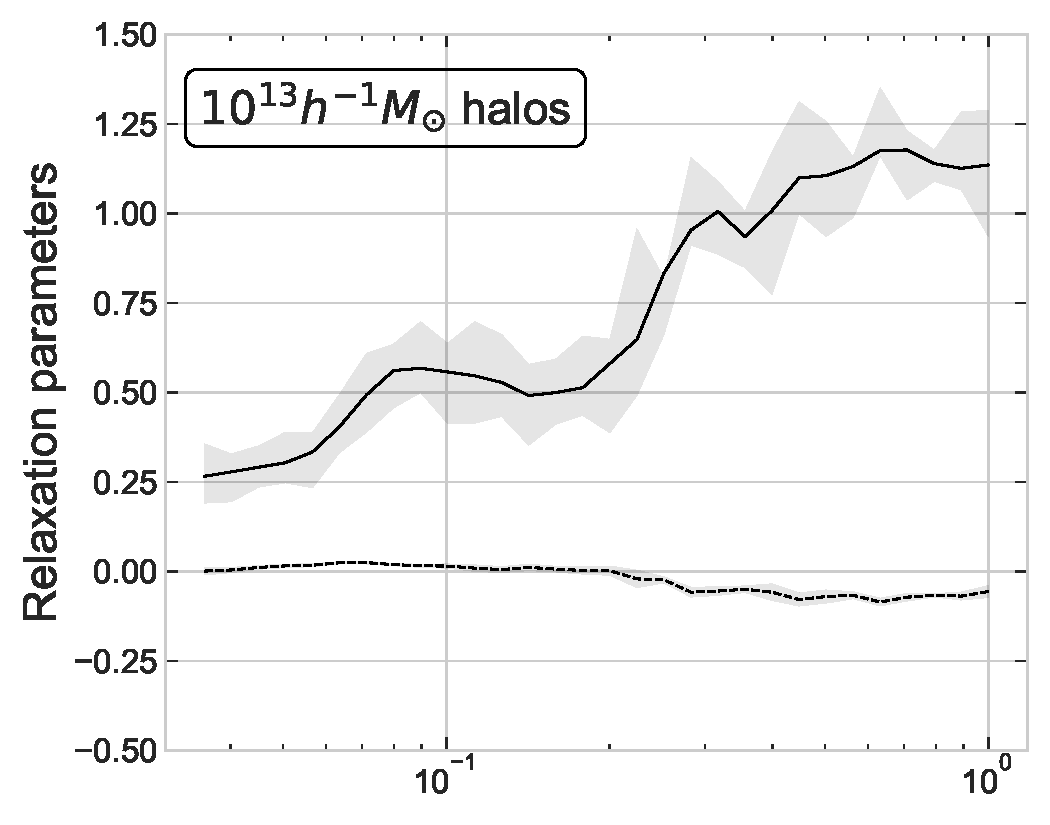
\includegraphics[width=0.32\linewidth]{plots/fit_params_rf_M_T_13.pdf}
    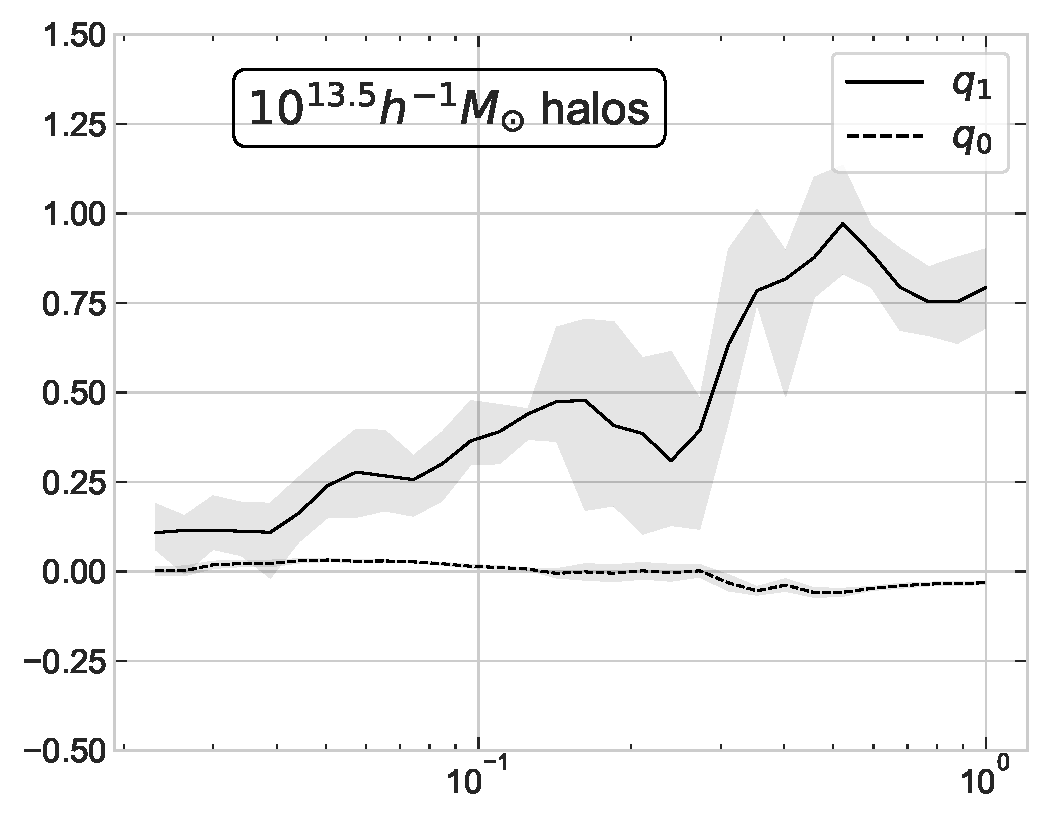
\includegraphics[width=0.32\linewidth]{plots/fit_params_rf_M_T_13.5.pdf}
    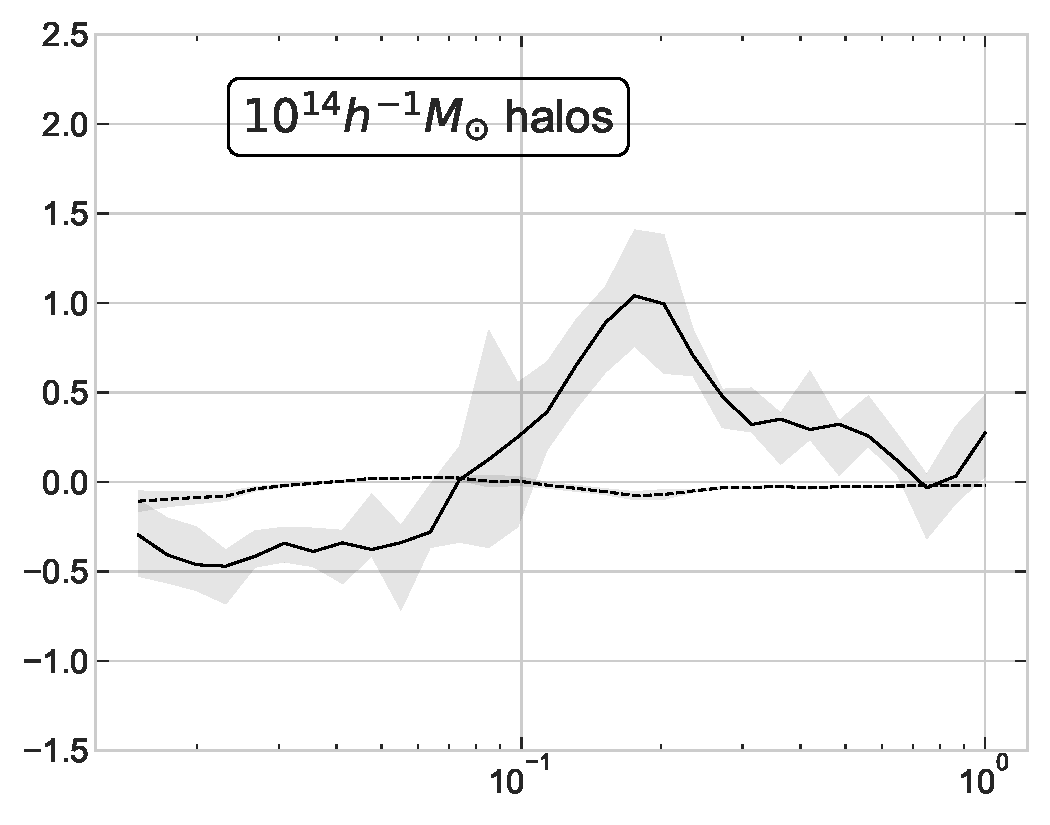
\includegraphics[width=0.32\linewidth]{plots/fit_params_rf_M_T_14.pdf}
    
    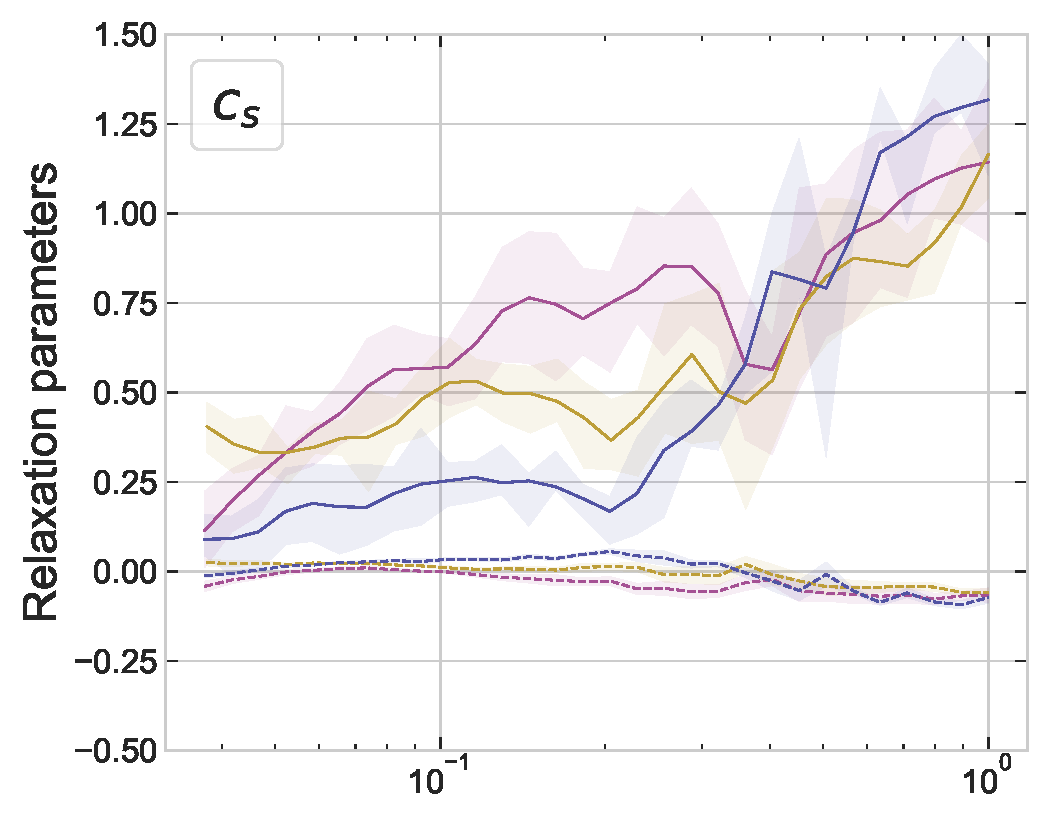
\includegraphics[width=0.32\linewidth]{plots/fit_params_rf_M-cs_T_13.pdf}
    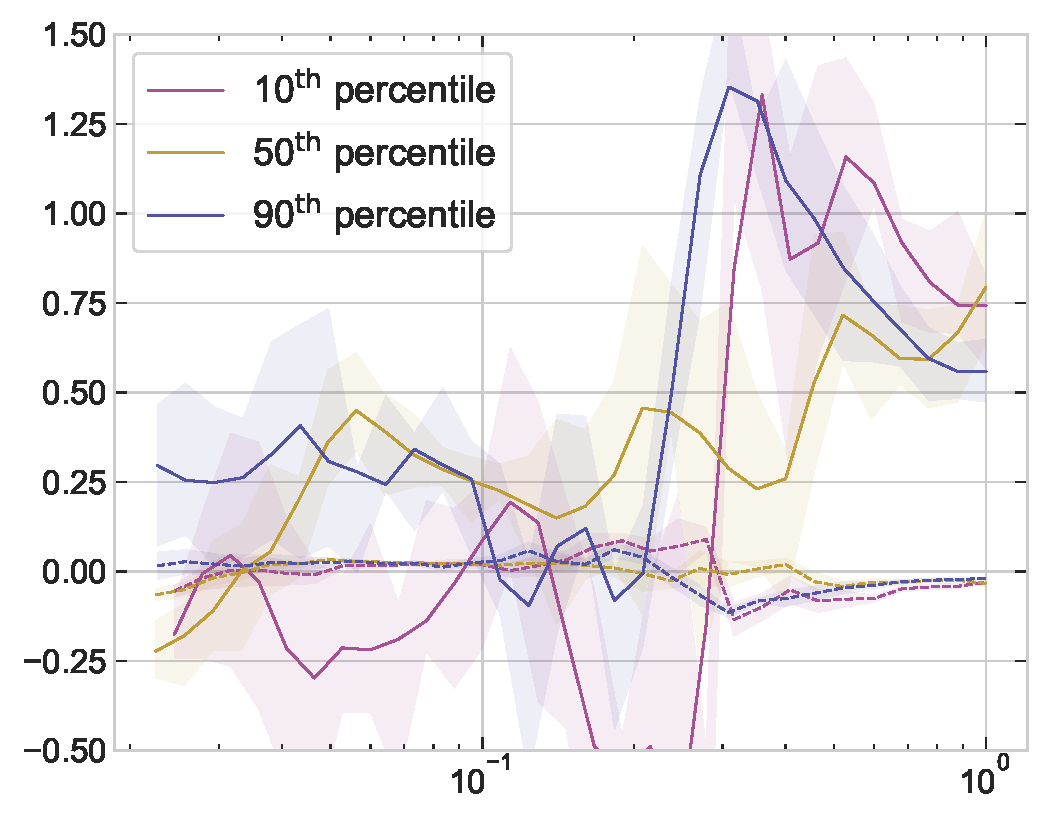
\includegraphics[width=0.32\linewidth]{plots/fit_params_rf_M-cs_T_13.5.pdf}
    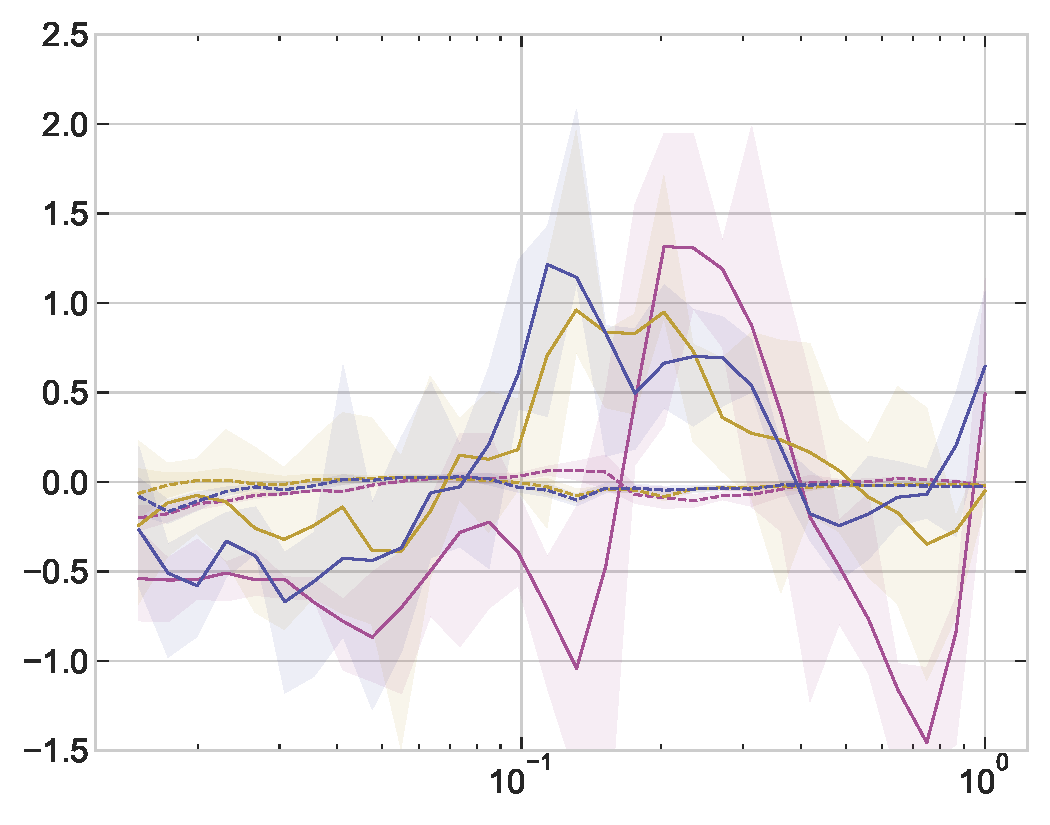
\includegraphics[width=0.32\linewidth]{plots/fit_params_rf_M-cs_T_14.pdf}
    
    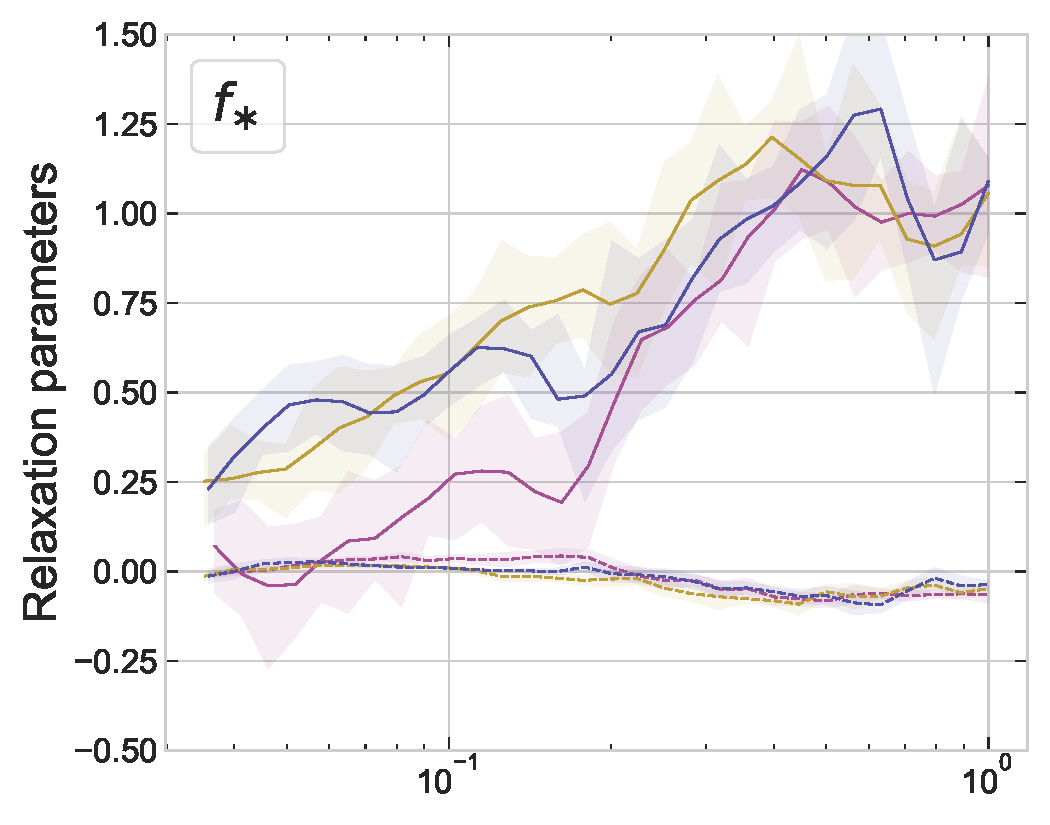
\includegraphics[width=0.32\linewidth]{plots/fit_params_rf_M-fs1_T_13.pdf}
    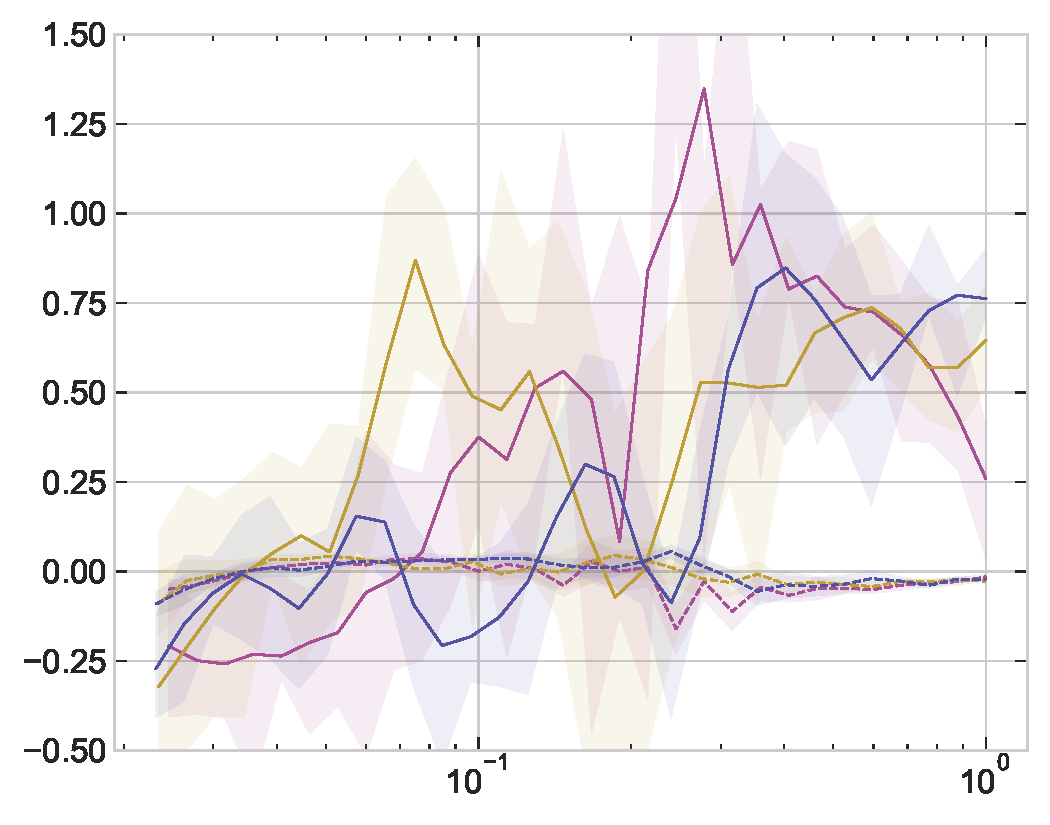
\includegraphics[width=0.32\linewidth]{plots/fit_params_rf_M-fs1_T_13.5.pdf}
    \includegraphics[width=0.32\linewidth]{plots/fit_params_rf_M-fs1_T_14.pdf}
    
    \includegraphics[width=0.32\linewidth]{plots/fit_params_rf_M-ssfr1_T_13.pdf}
    \includegraphics[width=0.32\linewidth]{plots/fit_params_rf_M-ssfr1_T_13.5.pdf}
    \includegraphics[width=0.32\linewidth]{plots/fit_params_rf_M-ssfr1_T_14.pdf}
    
    \includegraphics[width=0.32\linewidth]{plots/fit_params_rf_M-fg_T_13.pdf}
    \includegraphics[width=0.32\linewidth]{plots/fit_params_rf_M-fg_T_13.5.pdf}
    \includegraphics[width=0.32\linewidth]{plots/fit_params_rf_M-fg_T_14.pdf}
    
    \caption{Similar to upper panel of \figref{fig:rf-fit-params-ch:z0main} with cluster-scale haloes further split by other properties. In top row, only halo mass dependence is shown, whereas in the next three rows, we further show the dependence on halo concentration, stellar mass fraction, specific star formation rate and gas fraction in terms of percentiles respectively.} 
    \label{fig:fit-func-rf-13514-ch:z0main}
\end{figure*}





\section{Applications}
\label{sec:applic-ch:z0main}
In this section, we briefly discuss a few (potential) applications of our analysis.

\subsection{Baryonification schemes}

The results above show that the response of a halo's dark matter content to the galaxy and gas evolving in it depends not only on the integrated properties of the halo and galaxy (such as mass, concentration, etc.) but also on halo-centric distance, even at fixed mass ratio. This is in stark contrast to analytical approximations employed in the literature which typically use simplified  relations between the relaxation ratio and mass ratio, ignoring the radial dependence. These analytical approximations are now commonly employed in baryonification schemes to predict the total matter power spectrum for a given cosmological model using only the results of gravity-only $N$-body simulations \citep{2015JCAP...12..049S,2018MNRAS.480.3962C,2021MNRAS.503.3596A}. Our results above can directly impact such predictions by modifying the small-scale (deep 1-halo regime) behaviour of the power spectrum. 

For example, to model the effect of baryons in low- and intermediate-mass haloes ($\lesssim10^{13}\Mh$), we advocate the use of our fitting function \eqn{eq:q3-model-ch:z0main} for the relaxation relation, with parameters set to $q_0\simeq-0.05$, $q_{10}\simeq1.1$ and $q_{11}\simeq0.5$,\footnote{We have tested that the relaxed mass profile predicted by such a generic model agrees reasonably with the simulation; see \secref{sec:mass-prof-demo-ch:z0main} and \secref{sec:apndx-demo-ch:z0main} for a more accurate prediction} which gives a good description of the results of both IllustrisTNG and EAGLE haloes (see Fig.~\ref{fig:3-param-mass-only-ch:z0main}). For larger (cluster-sized) haloes, the response is still accurately described by the relation \eqn{eq:chi-linear-q0-ch:z0main}, but with more complex behaviour for the parameters $q_1(r_f)$ and $q_0(r_f)$, which presently needs to be accounted for numerically (see, e.g., Fig.~\ref{fig:fit-func-rf-13514-ch:z0main}). We discuss this further in \secref{sec:conclusion-ch:z0main}.









\subsection{Mass profiles}
\label{sec:mass-prof-demo-ch:z0main}
The primary utility of an analytical model (or fitting function) such as \eqn{eq:chi-linear-q0-ch:z0main} for the relaxation relation is to be able to predict the relaxed dark matter profile $M_f^d(r_f)$ of a halo which has responded to its baryonic content. The procedure for obtaining this profile is straightforward \citep[see, e.g., Appendix A of][]{2021MNRAS.503.4147P}: the relaxation relation is solved iteratively using the unrelaxed mass profile and the baryonic mass profile as inputs, until a converged answer for $M_f^d(r_f)$ is achieved.\footnote{In some cases, when these input profiles can be described by simplified analytical forms, a fully analytical expression for the relaxed dark matter profile can also be obtained \citep[see, e.g., Appendix A of][]{2021MNRAS.507..632P}.} In our case, the procedure to obtain the relaxed dark matter profile using \eqn{eq:chi-linear-q0-ch:z0main} works identically. The additional radial dependence of $q_1$ and $q_0$ is not an issue, since the radius $r_f$ itself is used as the control variable in solving for the enclosed mass.

\begin{figure}[htbp]
    \centering
    \includegraphics[width=0.84\textwidth]{plots/Mass-prof_with_demo_accu-1.pdf}
    \caption{\emph{(Top row:)} For the haloes in IllustrisTNG simulations, the mean radial mass profiles are shown in bins of halo mass for the baryonic component (dash-dotted curves) and dark matter component in hydrodynamic (dashed curves) and gravity-only (dotted curves) runs.  The relaxed dark matter mass profile predicted as described in \secref{sec:mass-prof-demo-ch:z0main} is shown by solid curves. The colour-coding follows Fig.~\ref{fig:mass_bin_label-ch:z0main}; for clarity we use two panels to show the averaged mass profiles for the nine mass bins. 
    \emph{(Bottom row:)} The ratio of the relaxed dark matter mass profile predicted by our model to that from the hydrodynamic simulation is shown by solid curves. For comparison, the corresponding ratio for quasi-adiabatic relaxation model with $q=0.33$ is shown by dashed curves and the ratio of dark matter mass profile between gravity-only simulation to the full hydrodynamic simulation is shown by dotted curves, representing the case of no relaxation. } 
    \label{fig:demo-fit-ch:z0main}
\end{figure}

As an example, we compare the relaxed profiles predicted by this procedure -- using the unrelaxed and baryonic mass profiles and the fits to the relaxation relation \eqn{eq:chi-linear-q0-ch:z0main} as inputs -- with the dark matter profiles actually measured in the hydrodynamical simulations for the same haloes.
For simplicity, in this analysis we ignore the dependence of the dark matter response on halo properties other than the mass;
we use $q_0$ and $q_1$ as a function of $r_f/R_{\rm{vir}}$ as shown in the \figref{fig:rf-fit-params-ch:z0main} for each halo mass bin. In the upper panel of Fig.~\ref{fig:demo-fit-ch:z0main}, we show this estimated mass profile along with the actual mass profiles found in the IllustrisTNG simulation.
For comparison, we also show the results of replacing the relaxation relation with simpler approximations from the literature (while still using the unrelaxed and baryonic mass profiles from the simulation as inputs in the iterative procedure).
Our model produces significantly better estimates of the relaxed dark matter profile, especially in the inner halo we obtain an order of magnitude better accuracy in comparison to such simple models (see lower panel of Fig.~\ref{fig:demo-fit-ch:z0main}). Below in \secref{sec:apndx-demo-ch:z0main}, we show that even the simple three parameter model gives a reasonably good prediction of the relaxed mass profile, while also being easier to incorporate into the existing procedures that use an adiabatic relaxation model. 



\subsection{Using the three parameter model}
\label{sec:apndx-demo-ch:z0main}
Here we show the relaxed mass profile predicted by our 3-parameter model \eqn{eq:q3-model-ch:z0main} for the haloes with mass, $M\leq10^{13}\Mh$. We follow a similar procedure as described above in \secref{sec:mass-prof-demo-ch:z0main}; once again we consider the response as a function of only the halo mass and ignore the dependence on other halo properties. For a given halo we obtain the values of the three parameters namely $q_0$, $q_{10}$ and $q_{11}$ by simply interpolating the fitted parameters shown in \figref{fig:3-param-mass-only-ch:z0main} as a function of mass. We find that accounting for radial dependence through a simple \eqn{eq:q3-model-ch:z0main}, gives a mass profile that is within $10\%$ of the simulation even upto $2 \%$ of virial radii (see upper left panel of \figref{fig:relxn_models_compare-ch:z0main}) and within $3 \%$ for the low mass haloes. The upper right panel of \figref{fig:relxn_models_compare-ch:z0main}, shows the corresponding profiles assuming a mass independent fixed values for the parameters $q_0\simeq-0.05$, $q_{10}\simeq1.1$ and $q_{11}\simeq0.5$. In addition to these, we also compare with mass profiles predicted by the standard adiabatic relaxation of Blumenthal et al. (1986) \citep{1986ApJ...301...27B} and few other relaxation models from Gnedin et al. (2004) \citep{2004ApJ...616...16G}, Paranjape $\&$ Sheth (2021) \citep{2021MNRAS.507..632P} and Cautun et al. (2020) \citep{2020MNRAS.494.4291C} for the IllustrisTNG haloes.

\begin{figure*}
    \centering
    \includegraphics[width=0.85\linewidth]{plots/relxn_model_comparison.pdf}
    \caption{Ratio of the relaxed dark matter mass profile predicted by various models to the dark matter profile found in the hydrodynamical simulation IllustrisTNG is shown by solid curves. Here the mass profiles are stacked across multiple haloes selected by their mass and the color coding follows \figref{fig:mass_bin_label-ch:z0main}. Results from our three parameter model \eqn{eq:q3-model-ch:z0main} is shown in the upper panel, while the left panel accounts for mass dependence in the parameters, the right panel assumes fixed values namely $q_0\simeq-0.05$, $q_{10}\simeq1.1$ and $q_{11}\simeq0.5$. In the rest of the panels, the corresponding ratio is shown for the mass profiles predicted by few existing models as mentioned in the \secref{sec:apndx-demo-ch:z0main}. The result from this work, as shown in bottom panel of \figref{fig:demo-fit-ch:z0main} is shown in dashed curves for reference.}
    \label{fig:relxn_models_compare-ch:z0main}
\end{figure*}


\subsection{Rotation curves}
Since our model can predict relaxed mass profiles using unrelaxed and baryonic mass profiles as inputs, it can also predict rotation curves of galaxies using the same inputs, along with some assumptions regarding the geometry of various mass components. 
The interpretation of observed rotation curves and related statistics such as the radial acceleration relation, using data from spatially resolved spectroscopy of nearby galaxies, forms a key aspect of discussions in the literature regarding the nature of gravity at galactic scales \citep[e.g.,][]{lms16b,lmsp17}. 

In the $\Lambda$CDM context, such studies typically model the relaxed dark matter profile using a generalised NFW profile, with or without a core, but unconnected to the baryonic mass \citep[e.g.,][]{llms20}. Previous work has suggested that the use of a parametrised model of dark matter \emph{response}, rather than the relaxed profile itself, should lead to more robust results \citep{2021MNRAS.507..632P,pscs21}. For example, it is known that the use of smooth NFW-like profiles does not produce formally good fits in cases where the observed rotation curve shows oscillatory behaviour. Rather, these oscillations in the rotation curve  correlate with similar oscillations seen in the measured baryonic mass profiles \citep[see, e.g., figs.~4 and~6 of][]{llms20}.\footnote{There could also be additional biases induced by various simplifying modelling assumptions regarding, e.g., circularity of orbits and disk thickness, which must be accounted for especially in the context of cored versus cuspy inner halo profiles \citep[see, e.g., the discussion in][]{roper+22}.} It is then reasonable to speculate that a model which smoothly parametrises the physics of the dark matter response, rather than the profile of dark matter itself, might account for such correlations naturally. More generally, such a model is more physically motivated than one which directly parametrises the dark matter profile itself. 

In a future work, we plan to confront observed rotation curves for low-mass systems with the 3-parameter relaxation model presented above. Our specific results for the values of these parameters in IllustrisTNG and EAGLE can then provide useful priors for the statistical comparison with data.












\section{Conclusion}
\label{sec:conclusion-ch:z0main}
In this chapter, we have explored in detail the response of the dark matter content of a halo to the galaxy and gas it hosts. Understanding and accurately modelling this response is important for a number of applications including baryonification schemes for small-scale power spectrum emulation, rotation curve modelling, %
constraining the nature of dark matter using inner halo mass profiles, etc. 

Using haloes and galaxies identified in the IllustrisTNG and EAGLE simulations and matched to their gravity-only counterparts, our analysis demonstrates that the simplified analytical schemes used thus far to model the dark matter response \citep[e.g.,][]{1986ApJ...301...27B,2010MNRAS.407..435A,2015JCAP...12..049S} are inadequate in describing its detailed behaviour across a variety of halo and galaxy types. Specifically, we showed that the dark matter response, or relaxation relation (see equation~\ref{eq:qAR1}), which connects the relaxation ratio $r_f/r_i$ to the mass ratio $M_i/M_f$ between unrelaxed (gravity-only) and relaxed (hydrodynamical) haloes, explicitly depends on halo-centric distance $r_f$ in the relaxed halo, in addition to being sensitive to a number of halo and galaxy properties including halo mass, halo concentration, stellar and gas mass fraction, and specific star formation rate. These effects, especially the dependence on halo-centric distance, have been typically neglected by existing quasi-adiabatic relaxation models. 

We presented a simple, physically motivated extension (equation~\ref{eq:chi-linear-q0-ch:z0main}) of the existing models which accurately captures the dark matter response over 4 orders of magnitude in halo mass ($10^{10}\lesssim M/(\Mh)\lesssim 10^{14}$) and $\sim2$ orders of magnitude in relative halo-centric distance ($0.02\lesssim r_f/R_{\rm vir}\leq1$). Apart from an explicit radial dependence of the relaxation relation (e.g., equation~\ref{eq:q3-model-ch:z0main} for low-mass haloes), a second novelty of our model is the inclusion of a parameter $q_0$ which characterises feedback-induced offsets seen in the relaxation relation measured in IllustrisTNG and EAGLE haloes in which, e.g., shells that do not show an overall change in radius ($r_f/r_i\simeq1$) nevertheless have $M_i/M_f>1$ (indicating loss of baryonic material). The existing quasi-adiabatic relaxation models do not allow for the existence of such shells, which are however captured well by our new null-offset parameter $q_0$ (see \secref{subsubsec:sim-relax-ch:z0main} for a detailed discussion).
We argued that our results could have a significant impact on the applications listed above.

Our analysis also raises some interesting questions, which we briefly discuss before concluding. We noted in \secref{sec:results-rad-dep-qadiab-ch:z0main} that, unlike low-mass haloes whose relaxation relation is well-described by \eqn{eq:q3-model-ch:z0main}, the radial dependence of the relaxation parameters $q_1$ and $q_0$ in \eqn{eq:chi-linear-q0-ch:z0main} for haloes with $M\gtrsim10^{13}\Mh$ shows non-trivial features and oscillations that are not easily captured by simple fitting functions (see Fig.~\ref{fig:fit-func-rf-13514-ch:z0main}). These features, which typically occur in the halo outskirts, are likely due to the presence of substructure or recent mergers, which would generically lead to a disturbed dynamical state of the halo. Here we have not attempted to model these features; it will be interesting in the future to systematically study the dependence of these features on substructure fraction, merger history, locations of shocks, etc.

At the other extreme, in the inner halo of low-mass systems, it is very interesting to ask whether the simple quasi-adiabatic relaxation prescription we have calibrated here can naturally lead to cored inner dark matter profiles. Previous attempts at coupling the relaxed dark matter profile to baryonic physics using simple prescriptions have focused on introducing a baryonic dependence of the parameters describing the dark matter profile itself \citep[e.g.,][]{2014MNRAS.441.2986D}. Our approach, on the other hand, parametrises the \emph{physics} of the dark matter response, and it will be interesting to see whether this leads to more robust results for cored inner profiles. For such an exercise, it will also be important to understand the dependence of our calibrated parameters on technical choices defining the sub-grid physics models used in the simulations, which can significantly impact the formation of cores \citep{bfln18}. We investigate the role of such sub-grid astrophysical models in \chapref{chap:physvar_z01}.

Finally, building a more in-depth understanding of our results will need a physical, preferably analytical, model. One possibility is to use the self-similar approximation \citep[][]{fg84,bertschinger85,launagai+15,shi16} to model the combined dynamical evolution of dark matter, gas and stars in a halo. We report the results of such a study in chapter \ref{chap:self-sim-relxn}.

 
% \section*{Acknowledgments}
% We thank Nishant Singh, Nishikanta Khandai and Kandaswamy Subramanian for useful discussions in the early phases of this work.
% We thank the anonymous referee for useful comments that improved the clarity of the presentation.
% We gratefully acknowledge the use of high performance computing facilities at IUCAA (\url{http://hpc.iucaa.in}). This work made extensive use of the open source computing packages NumPy \citep{vanderwalt-numpy},\footnote{\url{http://www.numpy.org}} SciPy \citep{scipy},\footnote{\url{http://www.scipy.org}} Matplotlib \citep{hunter07_matplotlib},\footnote{\url{https://matplotlib.org/}} Pandas \citep[][]{reback2020pandas},\footnote{\url{https://pandas.pydata.org/about/}} Schwimmbad \citep{schwimmbad},\footnote{\url{https://joss.theoj.org/papers/10.21105/joss.00357}} H5py,\footnote{\url{https://www.h5py.org/}} Colossus \citep{colossus},\footnote{\url{http://www.benediktdiemer.com/code/colossus/}}  Jupyter Notebook\footnote{\url{https://jupyter.org}} and Code-OSS.\footnote{\url{https://github.com/microsoft/vscode}}

% \section*{Data availability}
% The IllustrisTNG simulations are publicly available at \url{https://www.tng-project.org/}. The EAGLE simulations are publicly available at \url{https://icc.dur.ac.uk/Eagle/}. 


% \bibliography{references}

% \appendix












% \section{Locally linear relaxation relation}
 % 

\chapter[Role of Astrophysical Modeling on Dark Matter Halo Relaxation Response at Redshifts z=0 and z=1]{Role of Astrophysical Modeling on Dark Matter Halo Relaxation Response at Redshifts $z=0$ and $z=1$}
\label{chap:physvar_z01}

Advancements in computational cosmology have produced state-of-the-art hydrodynamical simulations of cosmological volumes with realistic galaxies (see, e.g., OWLS \citep{2010MNRAS.402.1536S}, Illustris \citep{2014MNRAS.445..175G}, FIRE \citep{2014MNRAS.445..581H}, EAGLE \citep{2015MNRAS.446..521S}, Horizon-AGN \citep[][]{2017MNRAS.467.4739K}, SIMBA \citep[][]{2019MNRAS.486.2827D}, IllustrisTNG \citep{2019ComAC...6....2N}). However, many sub-galactic astrophysical processes, such as star formation, are not resolved by these simulations. Instead, they rely on subgrid prescriptions with parameters calibrated to a set of empirical observations. Ambiguities in the modeling and the calibrated quantities have led to inconsistent results. Additionally, these simulations are computationally expensive to perform, which is why dark matter haloes have typically been studied using gravity-only simulations. Nevertheless, the impact of baryonic processes on the dark matter can be significant and must be accounted for before comparing against observations.

Early studies of individual haloes modeled the response of the radial distribution of dark matter to galaxy formation as adiabatic relaxation \citep[][]{osti6457593,1984MNRAS.211..753B,1986ApJ...301...27B,1987ApJ...318...15R}. However, this idealistic model rarely predicts the dark matter distribution within haloes in hydrodynamical cosmological simulations \citep[e.g.,][]{2004ApJ...616...16G,2010MNRAS.407..435A}. Moreover, the halo response was found to vary widely across haloes and in different simulations \citep[][]{2004ApJ...616...16G,2006PhRvD..74l3522G,2010MNRAS.402..776P,2010MNRAS.406..922T,2010MNRAS.405.2161D,2010MNRAS.407..435A,2011MNRAS.414..195T,2016MNRAS.461.2658D,2019A&A...622A.197A,2022MNRAS.511.3910F,2023Velmani&Paranjape}, leading to the development of various models of the response, some of which are direct extensions of adiabatic relaxation \citep[e.g.,][]{2004ApJ...616...16G,2006PhRvD..74l3522G,2010MNRAS.407..435A}. \AP{chapter heading at top left part of the page is showing `Introduction'? this may affect all chapters.}

In \chapref{chap:z0_main}, we have demonstrated that introducing an additional dependence on the halo-centric distance makes the relation between $r_f/r_i$ and $M_i/M_f$ linear across a variety of haloes in both IllustrisTNG and EAGLE simulations at the present epoch ($z=0$). Based on those results, we have presented a simple prescription for computing the relaxed dark matter mass profiles. In the first part of this chapter, we investigate if such a relaxation model can also be used at an earlier redshift.

Previous works have shown that feedback from various galactic processes strongly influences halo relaxation \citep{2011MNRAS.414..195T}. These effects primarily affect the offset in the relaxation relation, quantifying the excess relaxation experienced by the dark matter \citep{2023Velmani&Paranjape}. We have argued in \chapref{chap:z0_main}, that this could be the reason for the small deviations in the relaxation offset across haloes with different star formation activities. In this chapter, we systematically the role of various astrophysical processes in the galaxy, such as feedback, in mediating the relaxation response of the halo using simulations with variations in the feedback implementation.

This chapter is organized as follows. In \secref{sec:res-itng-z01}, we explore the relaxation response at an earlier redshift in the IllustrisTNG reference simulation. This allows us to understand how the different galactic processes occurring at earlier times affect dark matter halo relaxation. Then in \secref{sec:res-physvar-CAMELS}, we systematically study the relaxation response as a function of the feedback related parameters in the IllustrisTNG model using the set of simulations from CAMELS as described in \secref{sec:sims-CAMELS}. 
Following this, we investigate the role of a variety of astrophysical processes in the EAGLE physics variation simulations described in \secref{sec:sims-EAGLE} and conclude in \secref{sec:conclusion-ch:physvar}.

\section{Early epoch in IllustrisTNG simulations}
\label{sec:res-itng-z01}

In this section, we investigate the relaxation response in the radial distribution of dark matter in the main simulations of IllustrisTNG simulations at an earlier redshift of $z = 1$ and compare it to the present redshift of $z = 0$. Haloes at both these redshifts were identified and matched between hydrodynamical and the corresponding gravity-only runs as described in \secref{sec:hals}. Additionally, we use the SubLink merger tree catalogues to trace the most massive progenitor haloes at $z=1$ of the haloes considered at $z=0$. While present epoch haloes are sampled only by their masses at the present time, we consider three different methods for sampling the early epoch haloes. This results in four distinct sets of halo samples:

\begin{enumerate}
    \item $z=1$ haloes sampled by their masses at $z=1$.
    \item $z=1$ haloes sampled by the masses of their descendants at $z=0$. Note that not all haloes with a given mass at the present time have valid progenitors with the same mass at $z=1$.
    \item $z=1$ haloes sampled by their masses at $z=1$, but the mass bins are defined by the median masses of the most massive progenitors of the $z=0$ haloes.
    \item $z=0$ haloes sampled by their masses at $z=0$.
\end{enumerate}

In each case, the mass bins are defined as described in \secref{sec:results-mass-ch:z0main} considering the mass of the gravity-only halo. The representative colors to represent this halo mass is shown in \figref{fig:mass_bin_label-z01}. Additionally, this figure indicates the peak heights ($\nu$) corresponding to these halo masses at both $z=0$ and $z=1$. These values correspond to the rarity of haloes with that mass at that redshift with rarer haloes having larger values of $\nu$. This can be used to identify mass of the halo at $z=1$ that will have same rarity as $z=0$ halo of a given mass. 

For each of these four sets of halo samples, the average relaxation relations ($r_f/r_i$ vs $M_i/M_f$) are shown in \figref{fig:fit-view-mass-indep}. The bottom right panel, reproduces the \figref{fig:fit-view-mass-indep-ch:z0main} and shown here for comparison. We find that, for a given halo mass, relaxation is usually stronger at the earlier epoch (top left panel) compared to the present time $z=0$ (bottom right panel). In both cases, the trend in relaxation with halo mass is similar, with the strongest relaxation observed in $10^{12} \Mh$ haloes. Interestingly, cluster-scale haloes with masses of $10^{14} \Mh$ at redshift $z=1$ exhibit significant relaxation, unlike clusters of similar size at the present time.

The progenitors at redshift $z=1$ of the same haloes found at $z=0$ show even stronger  relaxation, especially in Milky Way-scale and larger haloes, as shown in the top right panel of \figref{fig:fit-view-mass-indep}. The relaxation follows the simple quasi-adiabatic model \eqref{eq:chi-linear-ch:sims} with $q=0.33$ among larger cluster-scale ($10^{14} \Mh$) haloes, while group-scale haloes are consistent with the second-order polynomial relation proposed by Abadi et al. (2010) \cite{2010MNRAS.407..435A}. In the bottom left panel, the relaxation relation is shown for all haloes within a narrow mass bin around the median mass of the progenitors of the haloes selected at $z=0$. Notice that the relaxation relation shifts further lower in Milky Way-scale haloes and smaller clusters with the inclusion of those additional haloes.

\begin{figure}[htbp]
\centering
\includegraphics[width=0.49\linewidth]{plots/Mass_bin_labels_z.pdf}
\caption{Representative colors denoting each of the halo mass bins. The numbers in the figure indicate the corresponding values of peak heights $\nu$ at redshifts $z=0$ and $z=1$.}
\label{fig:mass_bin_label-z01}
\end{figure}

\begin{figure*}
\centering
\includegraphics[width=0.48\linewidth]{plots/fit_view_M_T_snap049.pdf}
\includegraphics[width=0.48\linewidth]{plots/fit_view_M_T_snap049_smpl98.pdf}
\includegraphics[width=0.48\linewidth]{plots/fit_view_M_T_snap049_smpl98_allHalsMrange.pdf}
\includegraphics[width=0.48\linewidth]{plots/fit_view_M_T_snap098.pdf}
\caption{The stacked relation between relaxation ratio and mass ratio as a function of halo mass in IllustrisTNG at $z=0$ \emph{(bottom right panel)} and $z=1$ \emph{(other panels)}. In the top right panel, relaxation is shown at $z=1$ for the progenitors of the haloes selected at $z=0$. In the second row, left panel, relaxation is shown at different mass bins at $z=1$, indicated by corresponding mass bins at $z=0$. Points represent stacks over fixed halo-centric distances, and solid lines represent stacks over fixed mass ratios. The color-coding follows Fig.~\ref{fig:mass_bin_label-z01}. The quasi-adiabatic relaxation model \eqref{eq:chi-linear-ch:sims} with $q=0.68$ and $q=0.33$ are shown by the dot-dashed and dashed purple lines, respectively, in each panel.}
\label{fig:fit-view-mass-indep}
\end{figure*}

In \chapref{chap:z0_main}, we proposed a locally linear model of the relaxation relation as follows:
\begin{align}
\label{eq:chi-linear-q0-ch:physvar}
\frac{r_f}{r_i} - 1 &= q_1(r_f) \left[ \frac{M_i(r_i)}{M_f(r_f)} - 1 \right] + q_0(r_f),.
\end{align}
We have tested this relation with our halo samples at $z=1$ and found it to hold reasonably well. For each halo sample, at each $r_f$, the relationship between mass ratio and relaxation ratio across all haloes is fitted by a linear curve to obtain the parameters $q_0(r_f)$ and $q_1(r_f)$. These radial profiles of the relaxation parameters are shown in \figref{fig:rf-fit-params}.

The universality in these profiles extends to much larger mass haloes ($\sim 10^{13.5} \Mh$) at $z=1$ (top left panel) compared to $z=0$ (bottom right panel). This universality extends across all halo samples especially when considering all haloes identified by the median progenitor mass (shown in bottom left panel). Also we note that these radially-dependent relaxation results differ noticeably between bottom left panel and the top right panel. For example, in large clusters ($10^{14} \Mh$), the overall relaxation relation remains the same (black curves in \figref{fig:fit-view-mass-indep}), following the $q=0.33$ model. However, they differ when analyzed through the radially dependent relaxation model, as seen in \figref{fig:rf-fit-params} by comparing the black curves between the top right and bottom left panels. \AP{not sure about this... to me the black curves in bottom left and top right look very similar, except in the innermost parts of the halo}

The offset parameter $q_0$ shown in the lower subpanels is relatively uniform across the halo in all populations. The \figref{fig:fit-fit-func-q} shows the mean of $q_0$ in all four sets of halo samples. The $q_0$ parameter is usually more negative across all $z=1$ halo populations compared to $z=0$, indicating a stronger relaxation offset. Additionally, the values are more universal with halo mass at $z=1$. 

\AP{some physics discussion needed to explain differences seen between different samples}

\begin{figure}[htbp]
\centering
\includegraphics[width=0.48\linewidth,trim={0.5cm 0 0 0},clip]{plots/fit_params_rf_M_T_snap049.pdf}
\includegraphics[width=0.48\linewidth,trim={0.5cm 0 0 0},clip]{plots/fit_params_rf_M_T_snap049_smpl98.pdf}
\includegraphics[width=0.48\linewidth,trim={0.5cm 0 0 0},clip]{plots/fit_params_rf_M_T_snap049_smpl98_allHalsMrange.pdf}
\includegraphics[width=0.48\linewidth,trim={0.5cm 0 0 0},clip]{plots/fit_params_rf_M_T_snap098.pdf}
\caption{Linear quasi-adiabatic relaxation model parameters $q_1$ and $q_0$ as a function of the halo-centric distance at different halo masses in IllustrisTNG at $z=0$ \emph{(bottom right panel)} and $z=1$ \emph{(other panels)}. In the top right panel, relaxation is shown at $z=1$ for the progenitors of the haloes selected at $z=0$. In the second row, left panel, relaxation is shown at different mass bins at $z=1$, indicated by corresponding mass bins at $z=0$. The color-coding follows Fig.~\ref{fig:mass_bin_label-z01}.}
\label{fig:rf-fit-params}
\end{figure}

\begin{figure}[htbp]
\centering
\includegraphics[width=0.6\linewidth]{plots/fit_param_q0_M_T_z01.pdf}
\caption{Mean of the radially dependent quasi-adiabatic relaxation offset, $q_{0}$ as a function halo mass in the four sets of halo samples indicated by color.}
\label{fig:fit-fit-func-q}
\end{figure}










\section{Variation in astrophysical feedback using CAMELS simulations}
\label{sec:res-physvar-CAMELS}
In this section, we present the role of various feedback parameters prescribed in the IllustrisTNG simulations using the set of CAMELS simulations performed with the IllustrisTNG model. This includes a set of 41 hydrodynamical simulations, with one replicating the reference TNG model in a smaller cosmological volume, and 10 simulations each by varying 4 different feedback parameters as described in \secref{sec:sims-CAMELS}. To recall, this includes two supernovae feedback parameters ($A_{\mathrm{SN1}}$ and $A_{\mathrm{SN2}}$) and another two AGN feedback parameters ($A_{\mathrm{AGN1}}$ and $A_{\mathrm{AGN2}}$).

Due to the limited resolution and the smaller volumes of the CAMELS simulation, among all the mass bins shown in \figref{fig:mass_bin_label-z01}, we consider only $10^{11} \Mh$, $10^{11.5}$, and $10^{12} \Mh$ at both redshifts $z=0$ and $z=1$. Even in these mass bins, we consider only the outer well-resolved regions of the haloes. Also, since the cosmological volume is smaller than even the smallest TNG50 simulation, we have only a smaller sample of haloes at each of these halo mass bins. We find this sample size insufficient to estimate the radially-dependent relaxation parameters at each of these mass bins. We consider the following two approaches to alleviate this issue.

\subsection*{Intercepts in the Relaxation Relation}

The intercepts of the relaxation relation, given by the relation between $M_i/M_f-1$ and $r_f/r_i-1$, already provide interesting information about the relaxation. For example, the y-intercept denotes the offset in the relaxation ratio $r_f/r_i$ from unity for the shells having a mass ratio of unity $M_i/M_f=1$. Similarly, the x-intercept denotes the offset in the mass ratio $M_i/M_f$ from unity for the shells having a relaxation ratio $r_f/r_i = 1$.

In a given sample of haloes, we denote the average x and y intercepts as $q_x$ and $q_y$ respectively. For example, if we consider the Milky Way scale haloes at redshift $z=0$, the relaxation relation shown by the green curves in the lower right panel of \figref{fig:fit-view-mass-indep} indicates that $q_x$ will be positive and $q_y$ will be negative. In general, we expect that feedback effects would lead to larger $q_x$ and more negative $q_y$.

Due to the limited resolution of the CAMELS simulation, the outer well-resolved regions in most haloes didn't have a mass ratio less than unity. This makes the y-intercept of the relaxation relation available only in a smaller number of haloes. This makes our estimation of $q_y$ very noisy, and hence we only interpret the parameter $q_x$ in these simulations. This parameter $q_x$ is presented in \figref{fig:camels-qx0} as a function of the astrophysical parameters in the CAMELS TNG set of simulations at both redshifts $z=0$ and $z=1$.

\subsection*{Wider mass bin}

We found that the radially-dependent relaxation parameters are usually more uniform across a wider range of halo masses. We leverage this to consider haloes in a wider mass bin from $10^{11} \Mh$ to $10^{12} \Mh$, which gives a sufficient number of haloes to obtain the radially-dependent relaxation model parameters. However, still, the radial range is not sufficient to accurately model the radial dependence of the slope parameter $q_1(r_f)$, so we only investigate the offset parameter $q_0$, defined as the mean of the $q_0(r_f)$. This parameter $q_0$ is usually negative, and it is expected to be more negative when the offset produced by overall feedback effects is stronger. This model-dependent offset parameter is presented in \figref{fig:camels-q0q1} at both redshifts $z=0$ and $z=1$.

\begin{figure}[htbp]
\centering
\includegraphics[width=0.325\linewidth]{plots/CAMELS_I_qx0_sn18_11.pdf}
\includegraphics[width=0.325\linewidth]{plots/CAMELS_I_qx0_sn18_11.5.pdf}
\includegraphics[width=0.325\linewidth]{plots/CAMELS_I_qx0_sn18_12.pdf}
\includegraphics[width=0.325\linewidth]{plots/CAMELS_I_qx0_sn33_11.pdf}
\includegraphics[width=0.325\linewidth]{plots/CAMELS_I_qx0_sn33_11.5.pdf}
\includegraphics[width=0.325\linewidth]{plots/CAMELS_I_qx0_sn33_12.pdf}
\caption{Relaxation offset parameter $q_x$ \AP{axis labels say $q_{0}^x$ while text uses $q_x$} as a function of the baryonic astrophysical feedback parameters in haloes found in CAMELS-TNG at three different halo masses. Top: $z=1$, Bottom: $z=0$}
\label{fig:camels-qx0}
\end{figure}

\begin{figure}[htbp]
\centering
\includegraphics[width=0.49\linewidth]{plots/CAMELS_I_q0_sn18.pdf}
% \includegraphics[width=0.49\linewidth]{plots/CAMELS_I_q1_sn18.pdf}
\includegraphics[width=0.49\linewidth]{plots/CAMELS_I_q0_sn33.pdf}
% \includegraphics[width=0.49\linewidth]{plots/CAMELS_I_q1_sn33.pdf}
\caption{Relaxation offset parameter $q_0$ as a function of the baryonic feedback parameters in CAMELS-TNG. Left: $z=1$, Right: $z=0$.}
\label{fig:camels-q0q1}
\end{figure}

\subsection*{Discussion}

We find that among all haloes investigated, the feedback strength parameters $A_{\mathrm{SN1}}$ and $A_{\mathrm{AGN1}}$ have a strong influence on the relaxation, with $q_x$ typically increasing monotonically when increasing these parameters. On the other hand, 
%whereas 
the wind speed parameters $A_{\mathrm{SN2}}$ and $A_{\mathrm{AGN2}}$ have negligible effect on the relaxation characterized by both $q_x$ and $q_0$.


Recall that when varying only a wind speed parameter, it affects the burstiness of the feedback outflows while keeping the overall flux constant. Suppose the deviations in the relaxation relation from the idealized adiabatic model, quantified by non-zero offset parameters, are caused by the transfer of angular momentum between the dark matter particles and the baryonic particles. In that case, one may expect that the nature of the baryonic feedback quantified by the wind speed parameters will have a significant influence on the value of $q_x$. However, our results suggest otherwise.

This suggests that the strong influence of the overall feedback outflow flux on the relaxation is likely due to the time delay in the relaxation response of the halo. \AP{explain what this means. why is time delay relevant?} Also, the larger offsets characterized by $q_x$ in \figref{fig:camels-qx0}, with stronger feedback implementation, are consistent with our discussion in \secref{subsubsec:sim-relax-ch:z0main}. \AP{briefly describe how you infer this consistency}

We find that the AGN feedback strength generally has a stronger influence on the relaxation among the high-mass haloes, whereas the supernova feedback strength has a stronger influence in lower-mass haloes. This is consistent with our expectations that AGN feedbacks dominate in more massive haloes. However, at all masses, AGN feedback starts dominating the value of $q_x$ with unrealistically \AP{on what basis are these unrealistic? do we even care whether they are unrealistic or not? why mention this word?} strong AGN feedback implementations, indicated by the green curves in \figref{fig:camels-qx0}.

\AP{this para seems disconnected from previous one.}
The relaxation offset in the outer region of haloes characterized by $q_x$ is always larger with the stronger implementation of AGN feedback at both \( z=0 \) and \( z=1 \). However, in the slightly inner regions \AP{which part of which plot shows me the effect on these slightly inner regions, and why?}, stronger AGN feedback implementation leads to a weaker relaxation offset at \( z=0 \) and a stronger offset at \( z=1 \). \AP{are you talking about $q_0$ or $q_x$?} We interpret this as a consequence of the overall reduction in total feedback at \( z=0 \) due to the suppression of star formation caused by higher AGN feedbacks in the past. These results highlight the significance of feedback mechanisms in building a physical understanding of dark matter halo relaxation.

% We find that at $z=1$, the magnitude of $q_0$ is larger with stronger AGN feedback indicated by larger $A_{\rm{AGN1}}$. However, this trend is absent at $z=0$. This could be due to a strong suppression in star formation rate at the present epoch due to the stronger AGN feedback in the past. \AP{did you just forget to delete this para? it seems like a shorter and less informative version of the previous para. what is the point of this para?}









\section{Role of astrophysical models in EAGLE simulations}
\label{sec:res-physvar-eagle}

In this section, we present insights from small boxes of EAGLE simulations on the role of different feedback mechanisms on the relaxation response. These physics variation simulations from the EAGLE suite are described in \secref{sec:sims-EAGLE}. Again, due to the significantly smaller box size and resolution, we only consider haloes in three different mass bins centered at $10^{10.5} \Mh$, $10^{11} \Mh$, and $10^{11.5} \Mh$ as discussed in \secref{sec:res-physvar-CAMELS}. In these narrow mass bins, the mean relaxation relation obtained by stacking independent of the halo-centric distance is shown in \figref{fig:EAGLE-rad-indep} for these physics variation simulations. We find that the deviation in the relaxation across different astrophysical modeling is usually much smaller than the differences from one halo mass to the other. However, notice that the gas equation of state has a strong influence on the relaxation relation, especially among low-mass haloes. In particular, stiffer equations of state lead to a very large $r_f/r_i$ indicating a stronger expansion of the dark matter shells in response to galaxy formation.

In \figref{fig:EAGLE-rad-dep}, we present the radially dependent relaxation parameters for a larger sample of haloes in a wider range of halo masses from $10^{10.5} \Mh$ to $10^{11.5} \Mh$. These results also reflect the strong influence of the equation of state of gas on the relaxation response of dark matter haloes. Additionally, these results highlight the effect of supernovae feedback modeling. In particular, the $q_0(r_f)$ is more negative, indicating a stronger offset in the haloes found in the simulation with stronger supernova feedback implementation (brown curve vs. rose curve).    

\begin{figure}[htbp]
\centering
\includegraphics[width=0.32\linewidth]{plots/eagle_physvar_rad_indep_relxn_reln_MiMf_10.5.pdf}
\includegraphics[width=0.32\linewidth]{plots/eagle_physvar_rad_indep_relxn_reln_MiMf_11.pdf}
\includegraphics[width=0.32\linewidth]{plots/eagle_physvar_rad_indep_relxn_reln_MiMf_11.5.pdf}
\caption{Relaxation relation in the physics variation EAGLE simulations for haloes in the mass bins from $10^{10.5} \Mh$ to $10^{11.5} \Mh$. Here colors represent the specific simulation with a variation in the baryonic physics prescription.}
\label{fig:EAGLE-rad-indep}
\end{figure}

\begin{figure}[htbp]
\centering
\includegraphics[width=0.7\linewidth]{plots/fit_params_rf_M_E_physvar_fatmass_uniradb.pdf}
\caption{Radially-dependent relaxation parameters for low-mass haloes from $10^{10.5} \Mh$ to $10^{11.5} \Mh$ as a function of the halo-centric distance in the physics variation EAGLE simulations. Here colors represent the specific simulation with a variation in the baryonic physics prescription.}
\label{fig:EAGLE-rad-dep}
\end{figure}


\section{Conclusion}
\label{sec:conclusion-ch:physvar}

In this chapter, we investigated the influence of astrophysical modeling on the relaxation response of dark matter haloes at different epochs, specifically focusing on \( z=0 \) and \( z=1 \). The analysis is divided into three main parts, each shedding light on the role of various astrophysical processes in shaping the dark matter content of haloes.

% \subsubsection*{1. Early Epoch in IllustrisTNG Simulations}
We began by examining the relaxation response at an earlier redshift (\( z=1 \)) in the IllustrisTNG simulations using three distinct sets of halo samples, which highlight the variations in relaxation across different halo masses. Our study reveals that dark matter relaxation tends to be stronger (smaller \( r_f/r_i \)) at the earlier epoch compared to the present among haloes of the same mass. This is even more prominent among the progenitors of present epoch haloes. Notably, we observe that cluster-scale haloes at \( z=1 \) show significant relaxation (\( r_f/r_i < 1 \)) that is also a function of the change in the enclosed mass (\( M_i/M_f \)). This is in contrast to similar haloes at the present epoch, where \( r_f/r_i \) stayed close to unity on average irrespective of the value of \( M_i/M_f \).

We also find that the locally linear quasi-adiabatic relaxation model is a good description of the relaxation relation at this earlier epoch, demonstrating its robustness in capturing the dark matter response across redshifts. Moreover, the parameters of the radially dependent relaxation are found to be more universal across a much wider range of masses at \( z=1 \). For example, the progenitors of even the most massive clusters are well characterized by the simple three-parameter model of relaxation that was developed with a focus on galactic-scale haloes at \( z=0 \). \AP{speculate on why this is the case.}

% \subsubsection*{2. Variation in Astrophysical Feedback Using CAMELS Simulations}
Next, we explored variations in astrophysical feedback strengths within the IllustrisTNG model using simulations from the CAMELS project, which varies four different feedback parameters: two for stellar feedback and two for AGN feedback. Our analysis shows that the parameters controlling the energy flux of the feedback have a significant impact on the relaxation of dark matter at different epochs. In contrast, the parameters governing the speed and burstiness of feedback have negligible effects on the halo relaxation response. \AP{mention this is consistent with discussion of meaning of $q_0$}

We find that variations in stellar feedback strengths have a larger impact among dwarf galaxy-scale haloes, while variations in AGN feedback parameters exert a stronger influence on Milky Way-scale haloes. Notably, the relaxation offset in the outer well-resolved regions is stronger at the present epoch than at \( z=1 \), contrasting with results from the inner regions explored in the IllustrisTNG simulations in the first part of this chapter.

The stronger implementation of AGN feedback tends to result in greater relaxation at both \( z=0 \) and \( z=1 \) in the outer regions of the haloes. However, in the slightly inner regions, stronger AGN feedback implementation leads to a weaker relaxation offset at \( z=0 \) and a stronger offset at \( z=1 \). We interpret this as a consequence of the overall reduction in total feedback at \( z=0 \) due to the suppression of star formation caused by higher AGN feedbacks in the past. These results highlight the significance of feedback mechanisms in building a physical understanding of dark matter halo relaxation.

% \subsubsection*{3. Role of Astrophysical Models in the EAGLE Simulations}
Finally, we assessed the impact of different astrophysical models in the EAGLE simulations. Supernova feedback strengths show a similar trend to that observed in the CAMELS simulations. Additionally, we find that the gas equation of state has the strongest effect on the relaxation response of dark matter, particularly among haloes hosting dwarf galaxies.

Overall, this chapter underscores the intricate relationship between baryonic processes and dark matter halo relaxation, illustrating the variations that arise due to different astrophysical models and redshifts. % 

\chapter{Dynamics of the response of dark matter halo to galaxy evolution in IllustrisTNG}
\label{chap:dynam-relxn}


In the standard paradigm of cosmology, galaxies form within the gravitationally collapsed structures called haloes, primarily made of dark matter that doesn't interact with baryonic galaxies except through gravity \citep[][]{wr78}. Formation and the evolution of these haloes and the galaxies they host are crucial in both cosmological and astrophysical studies. However, the presence of baryonic matter introduces additional complexities. The gravitational coupling between baryons and dark matter can significantly alter the spatial distribution and evolution of the latter, necessitating a detailed study of this interaction. 

In \chapref{chap:z0_main}, we examined this impact of baryonic processes on dark matter haloes, focusing on the radial halo profiles in IllustrisTNG and EAGLE simulations across a wide range of halo masses at redshift $z \sim 0$. We found that simple adiabatic contraction models, which assume spherical symmetry and no shell crossing, often fall short of accurately describing the complex response of dark matter to baryonic effects observed in high-resolution hydrodynamical simulations.

However, by empirical modelling within the context of quasi-adiabatic relaxation, simple relations were found to describe the nature of the halo relaxation response. Building on those results, we systematically investigate the dynamical evolution of dark matter halo relaxation and its connection to the evolution of halo and galaxy properties. 

In this chapter, we use data from the IllustrisTNG simulation project towards this goal. By comparing the properties of haloes in the baryonic simulations of this suite with their counterparts in the corresponding gravity-only simulations, we characterize the relaxation behaviour of a variety of haloes across a wide range of masses over a time from redshift $z \sim 5$ to $z \sim 1$. We then perform multiple time-series analyses to determine the possible causal connections between the relaxation mechanism and astrophysical processes such as star formation and associated feedback processes, as well as feedback due to active galactic nuclei.

The structure of this chapter is as follows. We start with a brief description of the numerical simulations and the construction of a catalogue of matched haloes along with their evolutionary tracks in \secref{sec:simhals}. Then, in \secref{sec:methods-relchar}, we characterize the relaxation response in the context of a quasi-adiabatic framework and study their evolution in halo populations. This is followed in \secref{sec:methods-stat} by a statistical exploration of the connection between halo properties such as star formation rate and metallicity and their role in mediating the halo relaxation response. This analysis especially focuses on the rank correlations between these quantities not only across haloes in the populations but also over time. Finally, we conclude with a summary of our key findings and their applications in \secref{sec:conclusion}.


\section{Simulations of evolving pairs of haloes}
\label{sec:simhals}
Here we use all three different cosmological volumes of the publicly available IllustrisTNG simulations at their highest resolution \citep{2019ComAC...6....2N}; details of these simulations are outlined in \secref{sec:sims-IllTNG}. In this analysis, we utilise data from redshift $z=0$ all the way to redshift $z=5$ for both hydrodynamical and corresponding gravity-only runs. Haloes in these simulations were identified using a friend-of-friends (FoF) algorithm as described in \secref{sec:hals}. We match the haloes from the full hydrodynamic simulations with the haloes in the corresponding gravity-only runs as described in \secref{sec:hals}. From this catalogue, we select populations of matched halo pairs by the logarithmic mass of the gravity-only halo $(\log(M/\Mh))$ in bins centred at $11.5, 12, 12.5, 13, 13.5, 14$ with a bin width of 0.3 at redshift $z=0.01$. While the small volume TNG50 offers well-resolved low-mass haloes $10^{11.5} \Mh$ and $10^{12} \Mh$, the TNG100 cosmological box gives $10^{12.5} \Mh$ and $10^{13} \Mh$ haloes and the largest volume TNG300 provides an adequate number of cluster-scale haloes of masses $10^{13.5} \Mh$ and $10^{14} \Mh$. 

In cosmological simulations, it is particles that are evolved in cosmological volumes, and hence haloes need not be tracked explicitly. Rather, the haloes found at different snapshots in time are matched to construct the evolutionary tracks of the haloes. We identify the central subhaloes pairs corresponding to each pair of FoF group halos at $z\sim 0$ in our catalogue. These central subhaloes are traced back along the most massive progenitor branch using merger trees constructed by the \textsc{SubLink} code \citep{2015RodriguezGeneletalSubLink}. Then, the corresponding host FoF group haloes are considered as the progenitors of the matched haloes in our catalogue at $z \sim 0$. This gives us a catalogue of evolving pairs of haloes from redshift $z \sim 5$ to $z \sim 0$ corresponding to a cosmological look-back time of $12.63$ Gyr.

From this catalogue, we remove all those haloes that had a major merger during this period with a dark matter mass ratio above four. Further, we also remove those pairs of evolving haloes that are either separated by more than their virial radius or have sizes differing by more than $25\% $ at any given redshift. This leaves us with a sample of evolving matched haloes for around $50\%$ to $80\%$ of the populations of all haloes in our $z \sim 0$ catalogue. For these halo pairs, we study the relaxation by comparing the spherically averaged radial distribution of matter within their virial radii; this is described in  \secref{sec:methods-relchar}. Before that, we explore some of the key properties of these haloes in \secref{sec:hal-gal-props} that are relevant in this analysis.
% \PV{Mean evolution of some halo and galaxy properties plot}

\subsection{Astrophysical evolution}
\label{sec:hal-gal-props}
When it comes to the role of galactic astrophysical processes in mediating the halo relaxation, feedback processes are known to play a significant role \cite{2011MNRAS.414..195T,2023Velmani&Paranjape}. To understand this, we look into the astrophysical properties of the halo that quantify various galactic processes involved in producing the feedback. In this chapter, we primarily focus on the  following quantities: 
\begin{itemize}
    \item \textbf{SFR}: The net star formation rate of the central subhalo. The feedback associated with stellar winds and supernovae of massive stars follows star formation activity.
    \item $\mathbf{Z^{\star}_{\rm{O}}}$: The mean metallicity of oxygen in the star-forming regions within the central subhalo. Oxygen is a key tracer of chemical enrichment and feedback processes.
    \item $\mathbf{M_{\rm{Wind}}}$: The total mass of wind within the halo group. In addition to the stellar feedback, accretion onto AGN can also produce powerful winds. These winds eventually lose their mass and energy as they travel through the gas.
    \item $\mathbf{M_{\rm{O}}}$: The total oxygen content within the halo group in the gas component; This quantity probes the stellar feedback over a longer time, even after the suppression of $\mathbf{Z^{\star}_{\rm{O}}}$ due to inflowing metal-poor gas.
\end{itemize}
All these quantities are defined for the hydrodynamic halo of each matched group halo pair in our catalogue. The evolution history of these quantities in the populations of haloes having the same final mass is shown in \figref{fig:evolution-hal-gal-props}. While low mass haloes at $z \sim 0$ are currently at their peak star formation, it is significantly suppressed in the high mass haloes.

\begin{figure}[htbp]
\centering
\includegraphics[width=\linewidth]{plots/dynam_relxn/hal_gal_props_evolve.pdf}
\caption{Evolution history of the average star formation rate (SFR, top left panel), mean oxygen metallicity in star-forming regions ($Z^{\star}_{\rm{O}}$, top right panel), the mass of oxygen in gas ($M_{\rm{O}}$, bottom left panel) and mass of wind ($M_{\rm{Wind}}$, bottom right panel) in halo populations selected by their total mass at redshift $z\sim 0$ in the gravity-only run.}
\label{fig:evolution-hal-gal-props}
\end{figure}

\section{Time evolution of the halo response}
\label{sec:methods-relchar}
In \chapref{chap:z0_main}, we found that the relaxation relation follows a locally linear relation. 
\begin{align}
    % \label{eq:chi-linear-q0}
    \frac{r_f}{r_i} - 1 &= q_1(r_f) \left[ \frac{M_i(r_i)}{M_f(r_f)} - 1 \right] + q_0(r_f)\,.
\end{align}
For a given halo sample, at each $r_f$, the relation between mass ratio and relaxation ratio across all the haloes is fitted by a linear curve to obtain the parameters $q_0(r_f)$ and $q_1(r_f)$. It was also found that the $q_0(r_f)$ is usually roughly uniform from the inner to the outer haloes. \emph{Here we report that this radial dependent linear model is a good description of the halo relaxation over their evolution history back to at least redshift $z=5$} in populations of all six halo masses considered and at halo centric distance from the virial radius to at least $5 \%$ of that radius. To characterize the halo-to-halo variation in the relaxation offset, we define the following relaxation quantity for each halo in the population. 
\begin{align}
\label{eq:def-q0hal}
q_0 |_{h}(r_f) &\equiv \frac{r_f}{r_i} - 1 - q_1(r_f) \left[ \frac{M_i(r_i)}{M_f(r_f)} - 1 \right]\,.
\end{align}
This quantity $q_0 |_{h}(r_f)$ is usually uniform within each of the haloes; We primarily focus on its mean in this analysis, denoted simply as $q_0$ for that halo. We call this a relaxation offset parameter since it characterizes the amount of relaxation of dark matter shells that have no change in the total enclosed mass. In addition to this, we also study the mean $q_0(r)$ in the inner ($\sim 10\%~R_{\rm{vir}}$) and the outer ($\sim 50\%~R_{\rm{vir}}$) halo defined as $q_0^{\rm{in}} ~\& ~q_0^{\rm{out}}$ respectively.

\begin{figure}[htbp]
\centering
\includegraphics[width=\linewidth]{plots/dynam_relxn/hal_relxn_offset_evolve.pdf}    \caption{Dynamical evolution of the relaxation offset parameters $q_0$ (left panel) and $q_y$ (right panel) averaged in halo populations selected by their mass indicated by the same colour coding as in \figref{fig:evolution-hal-gal-props}}
\label{fig:evolution-hal-reln-offset}
\end{figure}
% \subsubsection{Model independent}
In addition to this model parameter $q_0$, we also define a somewhat model-agnostic quantity to characterize just the offset in the relaxation. \AP{you have already defined this in the previous chapter, right? then appropriately cite that definition instead of introducing it afresh here.} For each matched halo, the y-intercept of the relaxation relation is given by the relation between $M_i/M_f-1$ and $r_f/r_i-1$ for each matched halo. This parameter, denoted as $q_y$, is the offset in the relaxation ratio $r_f/r_i$ from unity for the shells having a mass ratio of unity $M_i/M_f=1$. The evolution history of these relaxation offset parameters for our halo populations is shown in \figref{fig:evolution-hal-reln-offset}. We find that the average evolution of $q_0$ and $q_y$ are similar for all haloes.  The relaxation offset starts with smaller values and reaches peak magnitudes before approaching zero, consistent with the $z \sim 0$ results presented in \chapref{chap:z0_main}. \AP{also say something to connect to the results of the previous chapter, else that chapter appears very neglected!} We have also checked that they show good correlation across haloes, especially $q_y$ shows good correlation with the $q_0^{\rm{in}}$. Hence, in this study, we will primarily focus the relaxation offset parameters $q_0(r)$,  $q_0^{\rm{in}} ~\& ~q_0^{\rm{out}}$.





\section{Statistical connections}
\label{sec:methods-stat}
The average evolution of the relaxation parameters shown in \figref{fig:evolution-hal-reln-offset} and other properties shown in \figref{fig:evolution-hal-gal-props} already suggest that the relaxation offset is strongest following the peak star formation period. However, we must study their evolution in individual haloes to further understand the role of different astrophysical processes. This additional information can be captured using correlations not only across haloes in the population but also over time between these quantities. In the \secref{sec:sfr-metallicity} below, we develop this methodology as we explore the connection between star formation rate and metallicity ($Z^{\star}_{\rm{O}}$) through these correlations. In the following (sub)section, we use this method to study the connection between relaxation and various galactic processes. 

\begin{figure}[bhtp]
\centering
\includegraphics[width=\linewidth]{plots/dynam_relxn/Spea_correl_betw_SFR-Z(O)_SFreg.pdf}
\caption{Correlation across haloes between star formation rate and metallicity ($Z^{\star}_{\rm{O}}$) in halo populations selected by their final masses at redshift $z\sim 0$. In the images, the colour at a given $(t[\rm{SFR}],t[Z^{\star}_{\rm{O}}])$ represents the Spearman rank correlation coefficient between the SFR at time $t[\rm{SFR}]$ and metallicity at time $t[Z^{\star}_{\rm{O}}]$ across haloes for each pair of times.}
\label{fig:dynam-correl-sfr-ZOsfr-img}
\end{figure}

\subsection{Star formation rate and metallicity connection}
\label{sec:sfr-metallicity}
As a warm-up, and as a means to showcase our method, we first present the correlation between the $Z^{\star}_{\rm{O}}$ and the SFR for haloes selected by their mass at redshift $z\sim 0$. 
In the simulation, metals are added to the gas by various feedback processes such as stellar winds and supernovae explosions that are dominantly produced by the short-lived massive stars. Hence, the metallicity is expected to rise following periods of star formation activity. To characterize this information, we focus on the Spearman rank correlations between the SFR and $Z^{\star}_{\rm{O}}$ at different times.

For a given population of $N$ haloes, we have the values of these two quantities for individual haloes tracked in distinct time steps $t_i$ with $i=1,2,\ldots,T$ separated by a uniform time interval $\Delta t = 157$ Myr. Using this, we construct the $T \times T$ matrix of Spearman correlation coefficients denoted by $\rho^s_{ij} [ \rm{SFR}, Z^{\star}_{\rm{O}}]$. Each element $ij$ of this matrix corresponds to the correlation between SFR at time $t_i$ with $Z^{\star}_{\rm{O}}$ at time $t_j$. (Note that the matrix is not expected to be symmetric.) Suppose $\rm{SFR}(n,t_i)$ and $Z^{\star}_{\rm{O}}(n,t_i)$ denote the corresponding quantities in the $n^{\rm{th}}$ halo at time $t_i$ in a population of $N$ haloes, then,
% 
\begin{align}
% \rho^s_{ij} [\rm{SFR}, Z^{\star}_{\rm{O}}] &= \rho^s [~\rm{SFR}(n \in [1,N],t_i), ~Z^{\star}_{\rm{O}}(n \in [1,N],t_j)~] \\%= \rho [R_{\rm{SFR}}(t_i), R_{Z^{\star}_{\rm{O}}}(t_j)]\\
% \intertext{\PV{Alternative notation}}
\rho^s_{ij} [\rm{SFR}, Z^{\star}_{\rm{O}}] &= \rho^s \left[~\rm{SFR}(\{1 \ldots N\},t_i), ~Z^{\star}_{\rm{O}}(\{1 \ldots N\},t_j)~\right] 
\end{align}
where the Spearman correlation $\rho^s$ is defined as the Pearson correlation ($\rho$) of the ranks ($R$), which in turn can be expressed as the covariance normalized by their standard deviations ($\sigma$).
\begin{align}
\rho^s_{ij} &[\rm{SFR}, Z^{\star}_{\rm{O}}] \\
&= \rho \left[~R[~{\rm{SFR}}(\{1 \ldots N\},t_i)~], ~R[~Z^{\star}_{\rm{O}}(\{1 \ldots N\},t_j)~]~\right]\\
&= \frac{\text{cov}\left(R[~{\rm{SFR}}(\{1 \ldots N\},t_i)~], R[~Z^{\star}_{\rm{O}}(\{1 \ldots N\},t_j)~]~\right)}{\sigma\left(R[{\rm{SFR}}(\{1 \ldots N\},t_i)]~\right) \times \sigma\left(R[Z^{\star}_{\rm{O}}(\{1 \ldots N\},t_j)]~\right)}\\
&= \frac{  (1/N) \sum_{n=1}^{N} R_{\rm{SFR}}(n,t_i) \times  R_{Z^{\star}_{\rm{O}}}(n,t_j) - \mu_{n} [ R_{\rm{SFR}}(n,t_i) ]  \times \mu_{n} [R_{Z^{\star}_{\rm{O}}}(n,t_j)] }
{ \sigma_{n} [ R_{\rm{SFR}}(n,t_i) ]  \times \sigma_{n} [R_{Z^{\star}_{\rm{O}}}(n,t_j)] }
\end{align}
% 
where $R_{\rm{SFR}}$ and $R_{Z^{\star}_{\rm{O}}}$ denote the corresponding ranks, while $\mu_n$ and $\sigma_n$ represent the mean and standard deviation, respectively computed across haloes ($n=1$ to $N$) at each time step. This matrix is depicted in \figref{fig:dynam-correl-sfr-ZOsfr-img} for the six populations of our evolving haloes selected by their final masses at $z \sim 0$; We find blue patches of strong positive correlation mostly near the diagonal. 
% \st{We find that there is a strong positive correlation between them at all halo masses indicated by the blue patches near the diagonal.} 
% \AP{i don't understand this argument. there are also red patches. and the diagonal is not always blue, e.g. for M=12.0. so at this point in the text how can you justify an overall positive correlation at all masses and all time lags?} \PV{It was a typo, I meant to say usually instead of overall} 
More specifically, there is usually a stronger positive correlation between the star formation rate at a given time and the $Z^{\star}_{\rm{O}}$ in the near future time. This is expected since the metals are primarily produced by the feedback that follows the star formation activity. 

Another thing to note is the strong negative correlation between the star formation rate of the haloes at later times with metallicity at a very early time and vice versa. 
% We have checked that this is also seen in the auto-correlation of the SFR 
% \st{This is also seen in the auto-correlation of the SFR and} \AP{i guess you are not showing this anywhere? in which case say something like `we have checked that this is also seen...'} \PV{We have checked but anyways I think it is not important to mention here.}
This happens at a characteristic time scale associated with the peak star formation period for that population of haloes. 
For example, in $10^{13} \Mh$ haloes, this transition period happens at a cosmic time of $2$ Gyr; this is indicated by the transition between blue and red patches. 
% \st{the haloes that were forming stars at a higher rate \underline{ended up}} \AP{are you guessing or do you have proof? if guessing then qualify with something like `likely ended up'} with lower star formation activity at later times. 
%(see \figref{fig:dynam-correl-sfr-ZOsfr-img}).
% 
While the metallicity is initially raised by the feedback events, the same feedback pushes inner metal-rich gas into the circumgalactic medium (CGM). On the other hand, the inflowing metal-poor gas from CGM lowers the metallicity while being crucial to feed the star formation activity at a later time. 
This leads to the inverse relationship between star formation rate and metallicity at fixed stellar mass reported in the literature \citep[][]{2011DaveFinlatorOppenheimer,2018TorreyVogelsberger_etal_SFRZ}; and our results are consistent with it.
% The gas inflow from CGM is usually followed by an enhanced star formation activity.
% The x-axis shows the time in scale factor at which the SFR is 
% In order to understand the halo and galaxy properties that are involved in mediating the relaxation, we look at the statistical correlation between the observed properties of those haloes in the simulation as a function of time. There are two different approaches 

\subsubsection{Correlation at fixed time intervals}
\label{sec:halhal-corr-sfrZ}
% \PV{Entire section rewritten} \\
We now focus on using the correlations to explore the repetitive nature of galactic processes. As a preliminary approach, we quantify this using the average of the Spearman rank correlation matrix $\rho^s_{ij}$ along the diagonals parallel to the black line shown in each panel of the \figref{fig:dynam-correl-sfr-ZOsfr-img}. This essentially represents the time-averaged correlation across haloes between SFR and $Z^{\star}_{\rm{O}}$ at a fixed earlier or later time, defined as:
%\AP{what exactly should the reader look at in the figure?} 
\begin{align}
\rho^s_h(\tau)[\rm{SFR}, Z^{\star}_{\rm{O}}] &= \avg{ \rho^s [ \rm{SFR}(t), Z^{\star}_{\rm{O}}(t+\tau)] }_{t}  
% \\ &=
% \begin{cases}
% \sum_{t_i=t_1}^{t_T-\tau} \rho^s [\rm{SFR}(t_i), Z^{\star}_{\rm{O}}(t_i+\tau)] \qquad \text{if } \tau \geq 0\\
% \sum_{t_i=\tau}^{t_T} \rho^s [\rm{SFR}(t_i), Z^{\star}_{\rm{O}}(t_i+\tau)] \qquad \text{if } \tau < 0
% \end{cases}
\end{align}
This quantity is computed at distinct time steps $(\tau=m \Delta t)$ for integer $m = 0,\pm 1,\ldots,\pm T$ using the matrix $\rho^s_{ij}$ as,
\begin{align}
\label{eq:def-hal-correl}
\rho^s_h(\tau = m \Delta t) 
&= \avg{ \rho^s_{i,i+m} }_i \\
&= \begin{cases}
\sum_{i=1}^{T-m} \rho^s_{i,i+m}/(T-m) \qquad \text{if } m \geq 0 \\
\sum_{i=1-m}^{T} \rho^s_{i,i+m}/(T-m) \qquad \text{if } m < 0
\end{cases}
\end{align}
Similar to the standard Spearman correlation coefficient, this quantity takes on a value between $-1$ and $+1$ at each $\tau$, indicating the strength of the correlation from being strongly negative to positive.
% As shown in \figref{fig:dynam-correl-sfr-ZOsfr-timeshift-func-halhal}, this quantity depicts that there is generally a stronger positive correlation between SFR with the future $Z^{\star}_{\rm{O}}$ in our halo population. This is clearly noticeable for the lowest (green curves) and highest halo masses (black and purple curves).
% Note that while this quantity averages over time, only the halo-to-halo correlation between the quantities is considered. This ignores the correlation between temporal variations in the star formation rate and metallicity. To capture that, we need to consider the correlation over time in their evolutionary tracks.
As shown in \figref{fig:dynam-correl-sfr-ZOsfr-timeshift-func-halhal}, this analysis reveals that the positive correlation is strongest between the SFR and the immediate future $Z^{\star}_{\rm{O}}$ as expected. Also, notice that on average, there is a stronger positive correlation $\rho^s_h$ for $\tau>0$ than $\tau<0$; This is particularly evident for the lowest (green curves) and highest halo masses (black and purple curves).
While there is a relatively stronger positive correlation at intermediate masses (blue curves), it is similar with both positive and negative time lags. This is a consequence of the fact that the $\rho^s_h(\tau)$ focuses only on the halo-halo correlation. Although $\rho^s_h(\tau)$ involves summation over both haloes and their evolutionary time steps, the ranks are computed independently at each of the time steps. Hence, it does not capture the correlation between temporal variations in the SFR and $Z^{\star}_{\rm{O}}$ of individual haloes, especially when the corresponding halo-to-halo variations are relatively stronger. In the following section, we present another quantity that can directly probe the correlations over time.


\begin{figure}[htbp]
\centering
\includegraphics[width=.6\linewidth]{plots/dynam_relxn/Spea_correl_vs_shift_betw_SFR-Z(O)_SFreg_halhalcorr.pdf}
\caption{Spearman correlation $\rho^s_h(\tau)$ across haloes between SFR and metallicity ($Z^{\star}_{\rm{O}}$) with a time lag. This is shown for the six populations of haloes selected by their final masses at redshift $z\sim 0$; Colour coding follows \figref{fig:evolution-hal-gal-props}.}
\label{fig:dynam-correl-sfr-ZOsfr-timeshift-func-halhal}
\end{figure}

\subsubsection{Time Correlations}
\label{sec:time-correl-sfrZ}
% \PV{Entire section rewritten} \\
In order to further understand the connection between the sequences of galactic processes, we study time correlations that capture the temporal variations along the evolutionary tracks of each halo.
% The halo-halo correlation might not capture the relevant information if the sample variance is either much smaller or larger than the temporal variations. 
Consider an individual halo along with its evolutionary track, say $n^{\rm{th}}$ halo in a population of N haloes. We characterize the time correlation through the Spearman correlation as a function of time lag, $\rho^s_t |_{n}(\tau)[\rm{SFR}, Z^{\star}_{\rm{O}}]$ defined as follows.
\begin{align}
\rho^s_t |_{n}(\tau)[\rm{SFR}, Z^{\star}_{\rm{O}}] &= \rho^s [ ~\rm{SFR}(n,t), Z^{\star}_{\rm{O}}(n,t+\tau) ~] \quad \text{where } ~t, t+\tau \in [t_1,t_T].
\end{align}
This quantity is also computed at distinct time steps ($\tau = m \Delta t$) for integer $m=0, \pm1, \ldots, \pm T$ as:
\begin{align}
\label{eq:def-time-correl-nth-halo}
\rho^s_t |_{n}(\tau = m \Delta t) &= 
\begin{cases}
\rho^s [ ~\rm{SFR}(n,\{t_1 \ldots t_{T-m}\}), ~Z^{\star}_{\rm{O}}(n,\{t_{1+m} \ldots t_T\}) ~]  \qquad \text{if } m \geq 0 \\
\rho^s [ ~\rm{SFR}(n,\{t_{-m+1} \ldots t_T\}), ~Z^{\star}_{\rm{O}}(n,\{t_1 \ldots t_{T+m}\}) ~] \qquad \text{if } m < 0
\end{cases}.
\end{align}

Alternatively, cross-correlation is also a characterization of the correlation over time in that halo. In particular, consider the cross-correlation function between the normalized ranks of SFR and $Z^{\star}_{\rm{O}}$ over its evolutionary history given by, 
\begin{align}
\rho^s_{t'} |_{n}(\tau = m \Delta t) 
% &= \sum_{} R^{\rm{norm}}_{\rm{SFR}}(n,t_i) \times R^{\rm{norm}}_{Z^{\star}_{\rm{O}}}(n,t_i)
&= \begin{cases}
\sum_{i=1}^{T-m} R^{\rm{norm}}_{\rm{SFR}}(n,t_i) \times R^{\rm{norm}}_{Z^{\star}_{\rm{O}}}(n,t_{i+m})/(T-m) \qquad \text{if } m \geq 0 \\
\sum_{i=1-m}^{T} R^{\rm{norm}}_{\rm{SFR}}(n,t_i) \times R^{\rm{norm}}_{Z^{\star}_{\rm{O}}}(n,t_{i+m})/(T-m) \qquad \text{if } m < 0
\end{cases}
\end{align}
where the normalized ranks are defined as
\begin{align}
R^{\rm{norm}}_{\rm{SFR}}(n,\{t_1 \ldots t_T\}) &= \frac{R[\rm{SFR}(n,\{t_1 \ldots t_T\})] - \avg{R[\rm{SFR}(n,\{t_1 \ldots t_T\})]}}{\sigma[R[\rm{SFR}(n,\{t_1 \ldots t_T\})]]},\\
R^{\rm{norm}}_{Z^{\star}_{\rm{O}}}(n,\{t_1 \ldots t_T\}) &= \frac{R[Z^{\star}_{\rm{O}}(n,\{t_1 \ldots t_T\})] - \avg{R[Z^{\star}_{\rm{O}}(n,\{t_1 \ldots t_T\})]}}{\sigma[R[Z^{\star}_{\rm{O}}(n,\{t_1 \ldots t_T\})]]}.
\end{align}
% These two quantities would agree at zero time-lag $\tau=0$, they ma

Both $\rho^s_t$ and $\rho^s_{t'}$ probe the time correlations, but they are not necessarily equal. To illustrate the difference, consider the $n^{\rm{th}}$ halo's evolutionary history over a period of 12 billion years. For a time-lag of 3 billion years between SFR and $Z^{\star}_{\rm{O}}$, $\rho^s_{t} |_{n}(\tau=3~\rm{Gyr})[\rm{SFR}, Z^{\star}_{\rm{O}}]$ is the Spearman correlation coefficient between SFR data from 12 billion years ago to 3 billion years ago and the metallicity from 9 billion years ago to the present. Here, the ranks, mean, and variance of the SFR are computed on the subset of data from 12 billion years ago until 3 billion years ago. As the average SFR evolves over time, the mean computed on this subset may differ from the mean SFR across the entire duration of 12 billion years. Therefore, the correlation function of the normalized ranks ($\rho^s_{t'} |_{n}(\tau=3~\rm{Gyr})[\rm{SFR}, Z^{\star}_{\rm{O}}]$) does not have to be equal to the actual Spearman correlation ($\rho^s_{t} |_{n}(\tau=3~\rm{Gyr})[\rm{SFR}, Z^{\star}_{\rm{O}}]$). The corresponding sample mean values of these two quantities of time correlations in each of the halo populations are defined as follows:
\begin{align}
\label{eq:def-time-correl}
\rho^s_{t}(\tau)[\rm{SFR}, Z^{\star}_{\rm{O}}] = \avg{ \rho^s_{t} |_{n}(\tau)[\rm{SFR}, Z^{\star}_{\rm{O}}] }_n, \\ 
\rho^s_{t'}(\tau)[\rm{SFR}, Z^{\star}_{\rm{O}}] = \avg{ \rho^s_{t'} |_{n}(\tau)[\rm{SFR}, Z^{\star}_{\rm{O}}] }_n.
\end{align}
% This is in contrast to $\rho^s_h(\tau)$ quantifying the time-averaged sample correlation across haloes in each population. 
% To address this, we define \(\rho^s_t(\tau)\), which quantifies the correlation over time along the evolutionary tracks of each halo, averaged across the population.

These time correlations ($\rho^s_t ~\&~ \rho^s_{t'}$) are shown by the solid and the dashed curves in the left panel of \figref{fig:dynam-correl-sfr-ZOsfr-timeshift-func-all} in each of our halo populations. While they agree at $\tau=0$, they deviate significantly as the time lag becomes larger than the timescales over which the local mean of the quantities evolve. In this analysis, we will only focus on the time lags where these two quantities are similar, as marked in the \figref{fig:dynam-correl-sfr-ZOsfr-timeshift-func-all}. In that case, we will consider the Spearman correlation as a function of time $\rho^s_t$; It takes on a value between $-1$ and $+1$, similar to the standard Spearman correlation coefficient. 
\begin{figure}[htbp]
\centering
\includegraphics[width=.49\linewidth]{plots/dynam_relxn/Spea_correl_vs_shift_betw_SFR-Z(O)_SFreg_timecorr.pdf}
\includegraphics[width=.49\linewidth]{plots/dynam_relxn/Spea_correl_vs_shift_betw_SFR-Z(O)_SFreg_fullcorr.pdf}
\caption{Spearman rank correlation coefficients, $\rho^s_t$ (left panel) and $\rho^s_f$ (right panel) as a function of the time lag between SFR and $Z^{\star}_{\rm{O}}$ for haloes selected by their final masses at redshift $z\sim 0$. Additionally, in the left panel the dashed lines indicate cross-correlation $\rho^s_{t'}$ as defined in the main text. Colour coding follows \figref{fig:evolution-hal-gal-props}. The horizontal lines indicate the time lag range that we interpret physically.}
\label{fig:dynam-correl-sfr-ZOsfr-timeshift-func-all}
\end{figure}

Notice that the positive time correlation $\rho^s_t>0$ is predominantly seen only with positive time lags $\tau>0$ even at the intermediate halo masses (see blue curves in \figref{fig:dynam-correl-sfr-ZOsfr-timeshift-func-all}). In general, at all halo masses considered, the SFR is correlated with the then future metallicity over a duration of atleast $2~\rm{Gyr}$. In addition, the time correlation also shows some more interesting information. It shows a significant anti-correlation between SFR and the \textbf{past} metallicity ($Z^{\star}_{\rm{O}}$) in most of our halo populations. This can again be interpreted in terms of lowering metallicity by the gas inflow from CGM, which also feeds the future star formation activity. 

The time correlation $\rho^s_t$ focuses on the temporal variations, but it doesn't consider the sample variation in the halo population. We define the full correlation, $\rho^s_f(\tau)$ by simultaneously correlating both across the sample of haloes and over their evolutionary tracks as follows:
\begin{align}
\rho^s_f (\tau)[\rm{SFR}, Z^{\star}_{\rm{O}}] &= \rho^s [ ~\rm{SFR}(n,t), Z^{\star}_{\rm{O}}(n,t+\tau) ~] \quad \text{where } n \in [1,N] ~\&~ t, t+\tau \in [t_1,t_T].
\end{align}
When computed at distinct time steps ($\tau = m \Delta t$) for integer $m=0, \pm1, \ldots, \pm T$, we have,
\begin{align}
\label{eq:def-full-corr}
\rho^s_f (\tau = m \Delta t) &= 
\begin{cases}
\rho^s [ ~\rm{SFR}(\{1 \ldots N\}, ~\{t_1 \ldots t_{T-m}\}), ~Z^{\star}_{\rm{O}}(\{1 \ldots N\}, ~\{t_{1+m} \ldots t_T\}) ~] \\
  \hfill \qquad \text{if } m \geq 0 \\
\rho^s [ ~\rm{SFR}(\{1 \ldots N\}, ~\{t_{-m+1} \ldots t_T\}), ~Z^{\star}_{\rm{O}}(\{1 \ldots N\}, ~\{t_1 \ldots t_{T+m}\}) ~] \\
 \hfill \qquad \text{if } m < 0
\end{cases}.
\end{align}
This considers $(T-m) \times N$ values of both SFR and $Z^{\star}_{\rm{O}}$ at each time lag $\tau = m \Delta t$; Suppose the ranks are denoted as $R^m_{\rm{SFR}}(n,t_i)$ and $R^m_{Z^{\star}_{\rm{O}}}(n,t_i)$, then for a positive value of $m$,
\begin{gather}
\rho^s_f (\tau = m \Delta t) = \nonumber\\
 \frac{ \sum_{i=1}^{T-m} \sum_{n=1}^{N} R^m_{\rm{SFR}}(n,t_i) \times  R^m_{Z^{\star}_{\rm{O}}}(n,t_j) - \mu_{n,t} [ R_{\rm{SFR}}(n,t_i) ]  \times \mu_{n,t} [R_{Z^{\star}_{\rm{O}}}(n,t_j)] }
{ N(T-m) \times \sigma_{n,t} [ R_{\rm{SFR}}(n,t_i) ]  \times \sigma_{n,t} [R_{Z^{\star}_{\rm{O}}}(n,t_j)] }
\end{gather}
where the mean ($\mu_{n,t}$), standard deviation ($\sigma_{n,t}$) and the ranks are computed over the $(T-m) \times N$ values,
\begin{align}
R^m_{\rm{SFR}}(\{1 \ldots N\}, ~\{t_1 \ldots t_{T-m}\}) &= R[ ~\rm{SFR}(\{1 \ldots N\}, ~\{t_1 \ldots t_{T-m}\}) ~]\\
R^m_{Z^{\star}_{\rm{O}}}(\{1 \ldots N\}, ~\{t_{1+m} \ldots t_T\}) &= R[ ~Z^{\star}_{\rm{O}}(\{1 \ldots N\}, ~\{t_{1+m} \ldots t_T\}) ~]
\end{align}
This full 2D Spearman correlation coefficient $\rho^s_f[\rm{SFR},Z^{\star}_{\rm{O}}]$ is presented in the right panel of the \figref{fig:dynam-correl-sfr-ZOsfr-timeshift-func-all}.
Once again, we only consider the range of time-lags marked in the figure at each of the halo masses. These are obtained by comparing $\rho^s_f(\tau)$ with the cross-correlation of normalized ranks computed on the entire duration and across all haloes in the population. We find that the full correlation $\rho^s_f$ tends to be stronger than the time correlation $\rho^s_t$, while also including the correlations in temporal variations unlike $\rho^s_h$ defined in \eqref{eq:def-hal-correl}.
% This will be useful later when studying the correlation between other quantities, especially when the underlying correlations are weaker. 
% Once again, we identify the range of time lags where the 
% \begin{align}
% \rho^s_f[\rm{SFR},Z](\tau) = \sum_{t_i=t_1}^{t_f-\tau} \sum_{n \in N} \rm{SFR}(n,t) \times Z(n,t+\tau)
% \end{align}


\subsubsection{Time lag analysis}
\label{sec:time-lag-analysis}
Spearman correlations ($\rho^s_h, \rho^s_t, ~\&~ \rho^s_f$) as a function time lag ($\tau$) as shown in figures \ref{fig:dynam-correl-sfr-ZOsfr-timeshift-func-halhal} and \ref{fig:dynam-correl-sfr-ZOsfr-timeshift-func-all} depict a qualitative picture of the sequences of galactic processes. In this section, we quantify the typical timescales associated with those processes. In this regard, we compute the mean time lag between SFR and metallicity weighed by their correlation strengths. This is done by considering the function of Spearman correlation coefficients in two regions of time lags: the correlation era $\rho_{+}$ and the anti-correlation era $\rho_{-}$.
\begin{gather}
\rho_{+}(\tau) = 
\begin{cases} 
\rho^s_f(\tau) & \text{if } \rho^s_f(\tau) > 0 \\ 
0 & \text{else} 
\end{cases}, \qquad
\rho_{-}(\tau) = 
\begin{cases} 
-\rho^s_f(\tau) & \text{if } \rho^s_f(\tau) < 0 \\
0 & \text{else} 
\end{cases}
\end{gather}
Then, for both the correlation and anti-correlation, we obtain the correlation weighted mean time lag ($\tau_{\pm}$), the mean correlation strength $A_{\pm}$ in that era and the time duration $\Delta\tau_{\pm}$
% \AP{i modified the notation from $d\tau_{\pm}$ to $\Delta\tau_{\pm}$. pls chk that it is changed everywhere.}
over which the correlation is significant.
\begin{gather}
\Delta\tau_{+} = \int_{\rho(\tau)>0} w d\tau , \qquad \Delta\tau_{-} = \int_{\rho<0} w d\tau   \\
A_{+} = \int w(\tau) \rho_{+}(\tau) d\tau / \Delta\tau_{+}, \qquad A_{-} = \int w(\tau) \rho_{-}(\tau) d\tau / \Delta\tau_{-} \\
\tau_{+} = \frac{1}{A_{+} \Delta\tau_{+}} \int \tau w(\tau) \rho_{+}(\tau) d\tau , \qquad \tau_{-} = \frac{1}{A_{-}\Delta\tau_{-}} \int \tau w(\tau) \rho_{-}(\tau) d\tau     
\end{gather}
Here, the weight function $w$ is taken to be the fraction of the entire data between $z \sim 5$ and $z \sim 0$ involved in computing the correlation coefficient at a given time lag. In general, the values of $\tau_{\pm}$ are physical only when the corresponding correlation strengths $A_{\pm}$ and the durations $\Delta \tau_{\pm}$ are both significant. Also note that when correlating between two quantities say $X$ and $Y$ a positive time lag $\tau_{+}[X,Y]$ (or $\tau_{-}[X,Y]$) indicate that the positive (or negative) correlation is seen with $Y$ lagging behind $X$. Hence the mean time lags are anti-symmetric with respect to the quantities, $\tau_{\pm}[X,Y]= - \tau_{\pm}[Y,X]$; However, the strengths and durations of correlations are symmetric, $A_{\pm}[X,Y]= A_{\pm}[Y,X]$ and $\Delta \tau_{\pm}[X,Y]= \Delta \tau_{\pm}[Y,X]$.

\begin{figure}[htbp]
\centering
% \includegraphics[width=.49\linewidth]{plots/dynam_relxn/shift_betw_SFR-Z(O)_SFreg_timecorr.pdf}
\includegraphics[width=.49\linewidth]{plots/dynam_relxn/shift_betw_SFR-Z(O)_SFreg_fullcorr.pdf}
\caption{In the top panel, correlation weighted mean time lags $\tau_{\pm}$ between SFR and $Z^{\star}_{\rm{O}}$ in the six halo populations selected by their final masses at redshift $z\sim 0$ are shown. The corresponding strengths $A_{\pm}$ and the durations $\Delta \tau_{\pm}$ of the correlation are shown in the middle and bottom panels, respectively.}
% Only the time correlations are considered in the left panel, while the right panel considers both sample and time correlation. \PV{shall one of them or combine them}}
\label{fig:dynam-correl-sfr-ZOsfr-timeshift-all}
\end{figure}

The mean time lags ($\tau_{\pm}$), the effective strengths ($A_{\pm}$) and the durations ($\Delta\tau_{\pm}$) of the correlation between the SFR and metallicity $(Z^{\star}_{\rm{O}})$ are shown in the \figref{fig:dynam-correl-sfr-ZOsfr-timeshift-all} for all our halo populations. 
% \AP{sign convention needs to be clarified, namely, the meaning of positive and negative values of $\tau$ when correlating quantity X with quantity Y. later you are using $\tau[X,Y]$, so why not just introduce that notation here and use it to clarify sign convention?}
The positive correlation between SFR and future $Z^{\star}_{\rm{O}}$ is depicted by positive values of $\tau_{+}[\rm{SFR}, Z^{\star}_{\rm{O}}]$. At low masses $(<10^{12.5}\Mh)$ this time lag is as large as $\tau_{+}=\sim 2 ~\rm{Gyr}$. At higher masses, though, the time lags are smaller, along with relatively lower correlation strengths. This is likely due to the strong AGN feedback redistributing the metals from the star-forming regions. In addition, the negative correlation identified qualitatively in the previous section can also be seen in the \figref{fig:dynam-correl-sfr-ZOsfr-timeshift-all} with large negative time-lags ($\tau_{-} \sim -3~ \rm{Gyr}$) in some halo populations (shown by dashed curves).
%\AP{weren't you going to explain that one should only seriously consider signals in regions where the correlation strength is high and the interval $\Delta\tau$ is significantly away from zero?}


\subsection{Interplay of halo relaxation with galactic processes}
\label{sec:main-res-halgal-relxn}
In this section, we study the correlations between the relaxation offset and various other properties of the halo/galaxy. To quantify the strength of the relaxation offset we define $Q_0 \equiv -q_0$; similarly we also define $Q_0^{\rm{in}}\equiv -q_0^{\rm{in}} \quad \& \quad  Q_0^{\rm{out}}\equiv -q_0^{\rm{out}}$ to characterize the strength of the relaxation offset in the inner and the outer regions of the halo respectively. Following the procedure described in the previous section, we primarily focus on the correlation-weighted time lags and their effective correlation strengths in this analysis.

\begin{figure}[htbp]
\centering
% \includegraphics[width=.49\linewidth]{plots/dynam_relxn/Spea_correl_vs_shift_betw_q0-SFR_fullcorr.pdf}
\includegraphics[width=.69\linewidth]{plots/dynam_relxn/shift_betw_multi-SFR_fullcorr.pdf}
% \includegraphics[width=.49\linewidth]{plots/dynam_relxn/Spea_correl_vs_shift_betw_q0(r)_in-SFR_fullcorr.pdf}
% \includegraphics[width=.49\linewidth]{plots/dynam_relxn/shift_betw_q0(r)_in-SFR_fullcorr.pdf}
% \includegraphics[width=.49\linewidth]{plots/dynam_relxn/Spea_correl_vs_shift_betw_q0(r)_out-SFR_fullcorr.pdf}
% \includegraphics[width=.49\linewidth]{plots/dynam_relxn/shift_betw_q0(r)_out-SFR_fullcorr.pdf}
\caption{In the top panel, correlation weighted mean time lags ($\tau_{\pm}$) between relaxation offset strengths ($Q_0, Q_0^{\rm{in}}, Q_0^{\rm{out}}$) against the star formation rate (SFR) in the six halo populations selected by their final masses at redshift $z\sim 0$ are shown. The corresponding strengths ($A_{\pm}$) and the durations ($\Delta \tau_{\pm}$) of the correlation are shown in the middle and bottom panels, respectively.}
\label{fig:dynam-correl-q0-SFR-timeshift-func}
\end{figure}

Let us start by studying the correlations between relaxation offset strengths and the SFR shown in the \figref{fig:dynam-correl-q0-SFR-timeshift-func}. In each case, a positive time lag of positive or negative correlation would mean that the corresponding correlation is seen with SFR lagging behind the offset strength; On the other hand, a negative time lag would indicate that the offset strengths lag behind the SFR with that correlation. We find that at all masses $Q_0$ shows a significant correlation with SFR over a long duration of $\Delta \tau_{+}\sim 6$ Gyr with $\tau_{+}$ close to zero. This is more prominent at high masses with effective correlation strength $A_{+}$ as high as $0.35$ at $10^{13.5} \Mh$. This is consistent with the results presented in \chapref{chap:z0_main} \AP{and Chapter 4?} where we have found that the relaxation offset to be stronger among haloes with higher specific star formation rate at redshift zero \AP{and $z=1$?}. In addition, we also see that at all masses except $10^{11.5}\Mh$, the mean time lag of positive correlation is negative with a magnitude as large as 1 Gyr in intermediate-mass haloes. This suggests that the higher star formation activity is followed by an enhanced relaxation offset. This means the past SFR is a better \AP{`better' than what? or do you just mean `good'?} predictor of the current relaxation offset.

Also notice that at all masses, $Q_0^{\rm{in}}$ shows a stronger correlation and with a higher time lag $\tau_{+}[Q_0^{\rm{in}},\rm{SFR}] > \tau_{+}[Q_0,\rm{SFR}]$. On the other hand, $Q_0^{\rm{out}}$ shows a significantly weaker correlation but with time lags $\tau_{+}[Q_0^{\rm{out}},\rm{SFR}] < \tau_{+}[Q_0,\rm{SFR}]$. This suggests that the astrophysical processes associated with star formation activity produce relaxation offset starting from the inner to the outer halo. The outer halo shows this positive correlation only for a shorter duration while negative correlation are stronger and seen for a longer duration ($\Delta \tau_{-}\sim 6 ~\rm{Gyr}$). With $\tau_{-}[Q_0^{\rm{out}},\rm{SFR}]>0$, this negative correlation with SFR is mostly seen over past relaxation offset in the outer halo.

% However, the inner relaxation offset is correlated with SFR in the more recent past compared to the outer relaxation offset, which is correlated to much earlier SFR. This is depicted in the figure by a more negative value of $\tau_{+}[\rm{SFR},Q_0^{\rm{out}}]$ compared to the $\tau_{+}[\rm{SFR},Q_0^{\rm{in}}]$ for high mass haloes. Also, we find this positive correlation to be much weaker in low-mass haloes than in high-mass haloes.

\begin{figure}[htbp]
\centering
% \includegraphics[width=.49\linewidth]{plots/dynam_relxn/shift_betw_SFR-Z(O)_SFreg_fullcorr.pdf}
% \includegraphics[width=.49\linewidth]{plots/dynam_relxn/Spea_correl_vs_shift_betw_q0-Z(O)_SFreg_fullcorr.pdf}
\includegraphics[width=.69\linewidth]{plots/dynam_relxn/shift_betw_multi-Z(O)_SFreg_fullcorr.pdf}
% \includegraphics[width=.49\linewidth]{plots/dynam_relxn/Spea_correl_vs_shift_betw_q0(r)_in-Z(O)_SFreg_fullcorr.pdf}
% \includegraphics[width=.49\linewidth]{plots/dynam_relxn/shift_betw_q0(r)_in-Z(O)_SFreg_fullcorr.pdf}
% \includegraphics[width=.49\linewidth]{plots/dynam_relxn/Spea_correl_vs_shift_betw_q0(r)_out-Z(O)_SFreg_fullcorr.pdf}
% \includegraphics[width=.49\linewidth]{plots/dynam_relxn/shift_betw_q0(r)_out-Z(O)_SFreg_fullcorr.pdf}
\caption{In the top panel, correlation weighted mean time lags ($\tau_{\pm}$) between relaxation offset strengths ($Q_0, Q_0^{\rm{in}}, Q_0^{\rm{out}}$) and SFR against the metallicity ($Z^{\star}_{\rm{O}}$) in the six halo populations selected by their final masses at redshift $z\sim 0$ are shown. The corresponding strengths ($A_{\pm}$) and the durations ($\Delta \tau_{\pm}$) of the correlation are shown in the middle and bottom panels, respectively.}
\label{fig:dynam-correl-q0-ZOsfr-timeshift-func}
\end{figure}

Moreover, the above result suggests that the effect of star formation activity on the relaxation offset is more immediate on the inner halo compared to the outer halo. This is consistent with the argument that the feedback from massive, short-lived stars that follow the star formation activities is causing the offset in the relaxation.  However, this also means that a measure of the recent feedback processes should correlate even more strongly with the relaxation offset strength. To test this, we have studied the correlations between the relaxation offset strengths and metallicity of oxygen in the star-forming regions ($Z^{\star}_{\rm{O}}$); this is shown in \figref{fig:dynam-correl-q0-ZOsfr-timeshift-func}

% the rate of increase in the oxygen mass in gas $M_{\rm{O}}' \equiv d M_{\rm{O}}/ dt$; this is shown in the \figref{fig:dynam-correl-q0-dMOFoF-timeshift-func}.


We find that the relaxation offset strength does show a positive correlation with $Z^{\star}_{\rm{O}}$, albeit weaker than the correlation found with SFR. 
% and also with an earlier time of $2 \rm{Gyr}$ 
With the exception of the highest halo masses, the positive correlation is first seen in the inner halo followed by the outer halo. This is depicted by 
\begin{align}
\tau_{+}[Q_0^{\rm{in}},Z^{\star}_{\rm{O}}] > \tau_{+}[Q_0^{\rm{out}},Z^{\star}_{\rm{O}}] > \tau_{+}[Q_0,Z^{\star}_{\rm{O}}]
\end{align}
Also, the correlations are relatively weaker for high-mass haloes where the correlation between SFR and $Z^{\star}_{\rm{O}}$ is also weaker. In $10^{13} \Mh$ haloes, there is a significant correlation with SFR ($A_{+}[\rm{SFR},Z^{\star}_{\rm{O}}] \sim 0.35$), but interestingly $Q_0$ correlates with much earlier $Z^{\star}_{\rm{O}}$ of over 4 Gyr in the past, while it correlates with SFR at just 1 Gyr in the past on average.
% we have \tau_{+}[Q_0^{\rm{out}},Z^{\star}_{\rm{O}}] close to - 4 Gyr indicating th
% \begin{algin}
% \tau_{+}[Q_0^{\rm{out}},Z^{\star}_{\rm{O}}] > \tau_{+}[Q_0^{\rm{out}},\rm{SFR}]
% \end{algin}
This may be because the feedback alone does not mediate the relaxation offset. At least we can say that the metallicity is not strongly associated with the feedback processes related to star formation activity involved in producing relaxation offset.

Since the metallicity in the star forming regions is also affected by the inflowing gas and redistribution by AGN feedbacks, we also study correlations with the overall rise in metals. In particular, let us now focus on the correlations between relaxation offset strengths and the rise in total oxygen mass in the gas content of the entire halo ($M_{\rm{O}}'$).  While $Z^{\star}_{\rm{O}}$ is an integrated quantity, $M_{\rm{O}}'$ tracks instantaneous increase in the metals. However, $M_{\rm{O}}'$ also shows only a weaker correlation with the relaxation offset compared to correlations with SFR (see \figref{fig:dynam-correl-q0-dMOFoF-timeshift-func}). We find that the loss of metals in the gas to the newly formed stars dominates over the metal enrichment by feedback. Hence SFR is negatively correlated with the future $M_{\rm{O}}'$ 
depicted by positive values of $\tau_{-}[\rm{SFR},M_{\rm{O}}']$.
% \AP{are you sure the negative sign isn't just because you switched sign convention compared to fig 6? i.e. are you actually plotting $\tau_{-}[M_{\rm{O}}',\rm{SFR}]$?} \PV{I have verified and the sign convention is same as fig 6; In both cases it is SFR first and then metallicity,  $\tau_{\pm}[\rm{SFR},Z^{\star}_{\rm{O}}]$ and $\tau_{-}[\rm{SFR},M_{\rm{O}}']$}

% Due to the We have then studied the correlations with the metallicity $Z^{\star}_{\rm{O}}$ of oxygen in the star-forming regions. We have already seen that this metallicity is an integrated quantity, and it has been correlated with the star formation rate over a long time. 
% However, this metallicity ($Z^{\star}_{\rm{O}}$) also shows only a weaker correlation with the relaxation offset compared to correlations with SFR (see \figref{fig:dynam-correl-q0-ZOsfr-timeshift-func}). 

Finally, we have also studied the correlations with the wind mass $M_{\rm{Wind}}$; this is presented in \figref{fig:dynam-correl-q0-Mwind-timeshift-func}. We find that the wind mass correlates with relaxation offset strengths in the future, affecting the inner halo earlier than the outer halo. We also find that the relaxation offset strength is correlated (although weakly) with the wind mass at a much later time in the future in low-mass haloes compared to high-mass haloes. We do see a similar trend in the correlation between wind mass and SFR; wind mass positively correlates with the star formation activity at a later time for lower mass haloes. However, we note that for the $10^{11.5}\Mh$ haloes, the wind mass correlates with the star-forming activity nearly 3.5 Gyr later. On the other hand, it correlates with the relaxation offset strength at just 2 Gyr in the future. Also, this correlation between wind mass and the relaxation offset is slightly stronger than the correlation we saw with SFR. This suggests that the wind mass is likely more closely associated with the relaxation offset than the star formation rate itself.

%\AP{what is the main result of this section? there is a collection of plots but no clear message. i had asked for typical numbers for the lag times in Gyr. pls report these wherever appropriate in the text for the main correlations studied here, because it is very difficult to read these off from the plots.}

% Since 

% metallicity of oxygen in the star-forming $Z^{\star}_{\rm{O}}$.
%  The total mass of wind within the FoF group halo $M_{\rm{Wind}}$.
%  The total oxygen content within the FoF group halo $M_{\rm{O}}$.

% In the \figref{fig:dynam-correl-q0-dMOFoF-timeshift-func}, , 


\begin{figure}[htbp]
\centering
% \includegraphics[width=.49\linewidth]{plots/dynam_relxn/Spea_correl_vs_shift_betw_q0-dM(O)_FoF_fullcorr.pdf}
\includegraphics[width=.69\linewidth]{plots/dynam_relxn/shift_betw_multi-dM(O)_FoF_fullcorr.pdf}
% \includegraphics[width=.49\linewidth]{plots/dynam_relxn/Spea_correl_vs_shift_betw_q0(r)_in-dM(O)_FoF_fullcorr.pdf}
% \includegraphics[width=.49\linewidth]{plots/dynam_relxn/shift_betw_q0(r)_in-dM(O)_FoF_fullcorr.pdf}
% \includegraphics[width=.49\linewidth]{plots/dynam_relxn/Spea_correl_vs_shift_betw_q0(r)_out-dM(O)_FoF_fullcorr.pdf}
% \includegraphics[width=.49\linewidth]{plots/dynam_relxn/shift_betw_q0(r)_out-dM(O)_FoF_fullcorr.pdf}
% \includegraphics[width=.49\linewidth]{plots/dynam_relxn/shift_betw_SFR-dM(O)_FoF_fullcorr.pdf}
\caption{In the top panel, correlation weighted mean time lags ($\tau_{\pm}$) between relaxation offset strengths ($Q_0, Q_0^{\rm{in}}, Q_0^{\rm{out}}$) and SFR against the rise in the oxygen mass in the gas ($M_{\rm{O}}'$) in the six halo populations selected by their final masses at redshift $z\sim 0$ are shown. The corresponding strengths ($A_{\pm}$) and the durations ($\Delta \tau_{\pm}$) of the correlation are shown in the middle and bottom panels, respectively.} 
% \AP{has the sign convention for correlation with SFR changed? why is $\tau_+ < 0$ for the purple solid line here but $>0$ in fig 6?}\PV{Same sign convention but fig 6 is for the metal fraction while this is for the change in the amount of metal and this quantity gets affected by absorption of metals into the stars}}
\label{fig:dynam-correl-q0-dMOFoF-timeshift-func}
\end{figure}




\begin{figure}[htbp]
\centering
% \includegraphics[width=.49\linewidth]{plots/dynam_relxn/Spea_correl_vs_shift_betw_q0-Wind_FoF_fullcorr.pdf}
\includegraphics[width=.69\linewidth]{plots/dynam_relxn/shift_betw_multi-Wind_FoF_fullcorr.pdf}
% \includegraphics[width=.49\linewidth]{plots/dynam_relxn/Spea_correl_vs_shift_betw_q0(r)_in-Wind_FoF_fullcorr.pdf}
% \includegraphics[width=.49\linewidth]{plots/dynam_relxn/shift_betw_q0(r)_in-Wind_FoF_fullcorr.pdf}
% \includegraphics[width=.49\linewidth]{plots/dynam_relxn/Spea_correl_vs_shift_betw_q0(r)_out-Wind_FoF_fullcorr.pdf}
% \includegraphics[width=.49\linewidth]{plots/dynam_relxn/shift_betw_q0(r)_out-Wind_FoF_fullcorr.pdf}
% \includegraphics[width=.49\linewidth]{plots/dynam_relxn/shift_betw_SFR-Wind_FoF_fullcorr.pdf}
\caption{In the top panel, correlation weighted mean time lags ($\tau_{\pm}$) between relaxation offset strengths ($Q_0, Q_0^{\rm{in}}, Q_0^{\rm{out}}$) and SFR against the mass in wind within the halo ($M_{\rm{Wind}}$) in the six halo populations selected by their final masses at redshift $z\sim 0$ are shown. The corresponding strengths ($A_{\pm}$) and the durations ($\Delta \tau_{\pm}$) of the correlation are shown in the middle and bottom panels, respectively.}
\label{fig:dynam-correl-q0-Mwind-timeshift-func}
\end{figure}


% \begin{figure}[htbp]
% \centering
% \includegraphics[width=.79\linewidth]{plots/dynam_relxn/shift_betw_multi-SFR_fullcorr.pdf}
% \includegraphics[width=.79\linewidth]{plots/dynam_relxn/shift_betw_multi-dM(O)_FoF_fullcorr.pdf}
% \caption{Correlation weighted mean time lag between model relaxation offset parameters $Q_0, Q_0^{\rm{in}}, Q_0^{\rm{out}}$ and other halo properties. Halo samples are selected by their final masses at redshift $z\sim 0$. Colour coding follows \figref{fig:evolution-hal-gal-props}. \PV{Merged plots} \AP{this is impossible to decipher. there are too many curves and the labels are illegible.}}
% \label{fig:dynam-correl-mainall-timeshift-func}
% \end{figure}

% \begin{figure}[htbp]
% \centering
% \includegraphics[width=.79\linewidth]{plots/dynam_relxn/shift_betw_multi-Z(O)_SFreg_fullcorr.pdf}
% \includegraphics[width=.79\linewidth]{plots/dynam_relxn/shift_betw_multi-Wind_FoF_fullcorr.pdf}
% \caption{Correlation weighted mean time lag between model relaxation offset parameters $Q_0, Q_0^{\rm{in}}, Q_0^{\rm{out}}$ and other halo properties. Halo samples are selected by their final masses at redshift $z\sim 0$. Colour coding follows \figref{fig:evolution-hal-gal-props}. \PV{Merged plots} \AP{this is impossible to decipher. there are too many curves and the labels are illegible.}}
% \label{fig:dynam-correl-mainall-timeshift-func}
% \end{figure}


% Key results q0 inner and outer are poorly correlated. However, the mean q0 is strongly correlated with qy. q0 and SFR show an interesting correlation that is more seen in inner q0 but not in outer q0. Correlation weighted time lag.

% \begin{itemize}
%     \item Correlation between metallicity and q0 outer halo shows a clear time offset in haloes of mass $\sim 10^{13.5} \Mh$.
% \end{itemize}

% \begin{table}[htbp]
% \centering
% \begin{tabular}{c|c|c|c}%
% \hline
% quantity & other quantity & halo mass & observation\\
% \hline &&&\\
% Z(O) & SFR & $10^{14}$ & SFR correlates strongly with metallicity  \\
%  & & to $10^{11.5}$ & especially at a slightly later time. (see figures \ref{fig:dynam-correl-sfr-ZOsfr-img},\ref{fig:dynam-correl-sfr-ZOsfr-timeshift-func-all}) \\
% Z(O) & q0 & $10^{14}$ & slightly negative correlation\\
% & & $10^{13.5}$ & \\
% \hline 
% \end{tabular}
% \caption{Results}
% \label{tab:results}
% \end{table}

% \subsection{Correlation between star formation rate and metallicity}

% \begin{figure}[htbp]
% \centering
% \includegraphics[width=.49\linewidth]{plots/dynam_relxn/Spea_correl_vs_shift_betw_SFR-Wind_sbhl_timecorr.pdf}
% \includegraphics[width=.49\linewidth]{plots/dynam_relxn/Spea_correl_vs_shift_betw_SFR-Wind_sbhl_fullcorr.pdf}
% \caption{Correlation between star formation rate and gas mass in the wind for haloes selected by their final masses at redshift $z\sim 0$.}
% \label{fig:dynam-correl-sfr-windsbhl-timeshift-func-all}
% \end{figure}







% Here we present the correlation between relaxation parameter $Q_0$ and star formation rate for haloes selected by their mass at redshift $z\sim 0$. 
% \begin{itemize}
%     \item We find that the inner q0 shows a good correlation with the increase in the total oxygen in the gas content of the halo and the star formation rate (SFR).
%     \item Meanwhile, outer q0 correlates with the metallicity of oxygen in the star-forming regions.
% \end{itemize}






\section{Conclusion}
\label{sec:conclusion}

This study explored the dynamical evolution of dark matter's response to galaxies within populations of haloes simulated using the IllustrisTNG cosmological volumes. By constructing a detailed population of haloes and tracing their evolutionary tracks, we characterized the relaxation response of these haloes. This was performed by comparing haloes from hydrodynamical simulations, which include subgrid prescriptions for various astrophysical processes, with corresponding haloes from gravity-only simulations. Using a catalogue of evolving matched haloes, we examined the correlation between relaxation quantities and other halo/galaxy properties to elucidate their roles in mediating the relaxation response.

Firstly, we find that the radially-dependent linear relaxation relation model is applicable even at earlier redshifts, at least from redshift $z=5$. In this chapter, we have primarily studied the offset parameter $q_0$ in the relaxation relation that characterizes the amount of relaxation of the dark matter shells with no change in the enclosed mass. In a given population of haloes selected by their final mass, this offset is on average stronger during the peak star formation among those haloes. 
Our findings reveal that star formation activity significantly influences the offset in the halo relaxation response  over the entire evolutionary history of the haloes. While this connection with SFR is immediate on the relaxation in the inner haloes, it is seen 2 to 3 billion years later on average in the outer regions of both Milky Way scale haloes and halo groups. %\AP{refer to typical lags mentioned in the prev section and compare with literature on SFR-metallicity.} 
%
We also found that simple tracers of the stellar feedback processes through metal content only show a weaker connection with the relaxation than SFR itself. However, the wind accumulated from various feedback processes did have a stronger connection with the relaxation.% While we expected that a  if the feedback processes traced by metals alone does not fully account for this offset. Notably, we observed a stronger correlation between the relaxation offset and the overall wind in the halo produced by various feedback processes. 

These insights enhance our understanding of the mechanisms driving halo relaxation and contribute to the development of more accurate models of halo profiles in baryonification procedures. 
% This has an important application barynification procedures and semi-analytic galaxy formation models. 
For example, the knowledge of time lags can, in princple, allow modelling the observed dark matter distribution in large surveys such as Euclid with fewer parameters by exploiting correlations across different redshift bins.
And in semi-analytic galaxy formation models, this %will
may allow simple time-dependent transformation procedures to incorporate the dynamical evolution of the host dark halo with galaxy evolution, which is typically ignored. In the future, the relaxation response of dark matter haloes can also serve as a probe into the evolutionary history of the galaxies they host.









% \bibliography{references,references_new}
% \newpage
% \appendix
% Appendix if anything requested by referee
% \section{Correlation between relaxation characteristic parameters}
% \label{sec:appen-q0qy}
% Here, we present the correlation between the model-dependent relaxation offset parameter $Q_0 \equiv -q_0$ and the model-independent relaxation offset parameter $Q_y \equiv -q_y$ for haloes selected by their final masses at redshift $z\sim 0$. We find that there is a strong positive correlation between them at all halo masses (see 
% \figref{fig:dynam-correl-q0-qy-timeshift-func}). Note that for small shifts in either direction, there is a steep dip in the correlation; this is also seen in the auto-correlation function of both $Q_y$ and $Q_0$.
% Also we find that the relaxation offset in the inner and outer halo are poorly correlated especially for the high mass haloes. 


% \begin{figure}[htbp]
% \centering
% \includegraphics[width=.49\linewidth]{plots/dynam_relxn/Spea_correl_vs_shift_betw_q0-qy_timecorr.pdf}
% % \includegraphics[width=.49\linewidth]{plots/dynam_relxn/shift_betw_q0-qy_timecorr.pdf}
% \includegraphics[width=.49\linewidth]{plots/dynam_relxn/Spea_correl_vs_shift_betw_q0(r)_in-qy_fullcorr.pdf}
% % \includegraphics[width=.49\linewidth]{plots/dynam_relxn/shift_betw_q0(r)_in-qy_fullcorr.pdf}
% \includegraphics[width=.49\linewidth]{plots/dynam_relxn/Spea_correl_vs_shift_betw_q0(r)_out-qy_fullcorr.pdf}
% % \includegraphics[width=.49\linewidth]{plots/dynam_relxn/shift_betw_q0(r)_out-qy_fullcorr.pdf}
% \includegraphics[width=.49\linewidth]{plots/dynam_relxn/Spea_correl_vs_shift_betw_q0(r)_in-q0(r)_out_fullcorr.pdf}
% % \includegraphics[width=.49\linewidth]{plots/dynam_relxn/shift_betw_q0(r)_in-q0(r)_out_fullcorr.pdf}
% % \includegraphics[width=.49\linewidth]{plots/dynam_relxn/Spea_correl_vs_shift_betw_q0-qy_halhalcorr.pdf}
% \caption{Correlation between model dependent relaxation offset parameter $Q_0$ and the model-independent relaxation offset parameter $Q_y$ for haloes selected by their final masses at redshift $z\sim 0$.\PV{Will remove vertical lines}}
% \label{fig:dynam-correl-q0-qy-timeshift-func}
% \end{figure}
















% \end{document} % 

\chapter{A self-similar model of galaxy formation and dark halo relaxation}
\label{chap:self-sim-relxn}

The most realistic description of halo relaxation response in the presence of baryons is provided by hydrodynamical simulations that include calibrated effects of star formation, radiative cooling, feedback due to stellar winds and supernovae as well as the triggering of AGN activity in super-massive black holes and its feedback on star formation. In the previous chapter, we quantified this response in such simulations by studying the mass profiles of matched pairs of halos in the hydrodynamical and gravity-only runs of the simulation. In the quasi-adiabatic relaxation framework, we further provided convenient fitting forms for this parametrised relaxation.

In this chapter, we investigate whether we can gain some physical insights into the problem of halo relaxation due to baryonic backreaction using a more tractable, spherically symmetric self-similar model (see \secref{sec:intro_self_sim}). We expect the insights gained from this approach will be useful in building physically interpretable models of relaxation.

The assumption of self-similarity reduces the nonlinear coupled partial differential equations into ordinary differential equations. This uses a scale radius that evolves over time to relate spatial variations to the temporal variations. Building on the self-similar models, we incorporate two novel additions: (i) a self-similar cooling of the gas and (ii) the formation of a pseudo-disk of gas along with the self-similar collapse of the dark matter halo. Unlike the work of Bertschinger (1989) \citep{1989Bertschinger}, where the cooling scale was set by a cooling radius and was primarily applicable to the innermost regions, in our model we set the cooling scale relative to the turn-around radius. This allows us to keep intact the global self-similarity of the model, while allowing for a range of possible amplitudes for the cooling rate.

\emph{Importantly, we self-consistently solve for the evolution of the gas and the dark matter simultaneously using a novel iterative technique.} This approach allows us to reliably estimate the relaxation of the dark matter due to baryonic backreaction in this self-similar model. The inclusion of cooling and the formation of a pseudo-disk also brings our self-similar model of galaxy formation substantially closer to the more realistic results of hydrodynamical simulations. We leave the incorporation of the formation of stars and a central black hole, and the associated stellar and AGN feedback, to future work.

This chapter is organised as follows. We outline the self-similar model of dark matter halo collapse in \secref{sec:methods-dm-ch:ssr}. Then we construct our new self-similar galaxy formation model in \secref{sec:methods-gas-ch:ssr} followed by its co-evolution with dark matter in an EdS universe in \secref{sec:methods-interplay-ch:ssr}. Then, we discuss the solutions to our self-similar galaxy formation model in \secref{sec:results-gaso-ch:ssr}. Following this we present the self-similar solutions in our model of co-evolving dark matter halo and gas accretion onto a galaxy in \secref{sec:results-gas-dm-coevolve-ch:ssr}. In this section, we discuss the relaxation response of dark matter halo in this self-similar setting and compare against the results from simulations and we conclude in \secref{sec:conclusion-ch:ssr}.





\section{Self-similar model of dark matter infall}
\label{sec:methods-dm-ch:ssr}
We start with an outline of the self-similar spherical collapse model of the self-gravitating dark matter halo in the EdS universe. We describe our model of galaxy-halo co-evolution in the following (sub)sections. The evolution of spherical shells with physical radius $r(t)$ under the gravitational influence of the mass enclosed is given by, 
\begin{align}
\label{eq:dm_traj_phys_accl-ch:ssr}
\frac{\der^2 r}{\der t^2} = - \frac{GM(r,t)}{r^2}.
\end{align}
Their trajectories can be solved analytically using Lagrangian coordinate as long as those shells don't cross each other; that is for a shell at radius $r_i$ at some early time $t_i$ with velocity $v_i$, the \eqn{eq:dm_traj_phys_accl-ch:ssr} can be integrated until the enclosed mass remains same as the initial mass $M_i$,
\begin{align}
\label{eq:dm_traj_phys_ener-ch:ssr}
\left( \frac{\der r}{\der t} \right)^2 - v_i^2 = \frac{2GM_i}{r} - \frac{2GM_i}{r_i}\,,
\end{align}
which simply represents conservation of energy for each shell.
Further by expressing the enclosed mass $M_i$ in terms of the overdensity in the sphere enclosed by the shell above the critical density $\rho_H(t_i)$, we have
\begin{align}
\nonumber
\delta_i \equiv \delta M_i / M_i \implies \frac{2GM_i}{r_i} = \frac{2G \rho_H(t_i)}{r_i} \frac{4}{3}\pi r_i^3 (1+\delta_i) = r_i^2 H_i^2 (1+\delta_i).
\end{align}
where $H_i$ denotes the initial value of the Hubble parameter $H=2/(3t)$ in the EdS universe. Further assuming the shells follow Hubble flow initially
($v_i^2 = r_i^2 H_i^2$), 
the \eqn{eq:dm_traj_phys_ener-ch:ssr} gives analytical solution for the trajectory of all the shells \cite{1993paddy_strucformbook},
\begin{gather}
\left( \frac{\der r}{\der t} \right)^2 = \frac{2GM_i}{r} - r_i^2 H_i^2 \delta_i,\\
\label{eq:dm_traj_soln_phys-ch:ssr}
r(\theta) = (1 - \cos \theta) G M_i/r_i^2 H_i^2 \delta_i \qquad t(\theta) = (\theta - \sin \theta) G M_i/r_i^3 H_i^3 \delta_i^{3/2}.
\end{gather}
Each shell expands initially but then turns around at a radius of $r_{\smallfrown}= 2G M_i/r_i^2 H_i^2 \delta_i$ at time $t_{\smallfrown} = \pi G M_i/r_i^3 H_i^3 \delta_i^{3/2}$ that is specific to that shell. 
However, as a dark matter shell falls into the halo after this turnaround,
its trajectory starts to deviate from this solution when crossing other collisionless dark matter shells that are expanding outwards from the centre. 
Moreover, these shells turn around once again and start accreting as a secondary infall. This leads to the formation of caustics such as the splashback radius. 

Even in such regions, self-similar solutions are obtained assuming scale-free initial perturbation with a power law form of overdensity distribution $\delta_i \propto M_i^{-\epsilon}$ \cite{1984FillmoreGoldreich}. For sufficiently larger scales, with small perturbation $\delta_i \ll 1$, we can write $M_i \propto r_i^3$ and hence 
$r_{\smallfrown} \propto M_i^{1/3+\epsilon}$ \& $t_{\smallfrown} \propto M_i^{3\epsilon/2}$. At any given time $t$, the shell that undergoes turnaround, encloses a mass of $M_{\smallfrown} \propto t^{2/3\epsilon} \propto a^{s}$, where $s=1/\epsilon$ is the mass accretion rate of the halo; hence this parameter $s$ relates to both the nature of initial perturbation and the accretion rate. It follows that the (turnaround) radius of such a shell undergoing turnaround at any time $t$, has a simple power law evolution $r_{\smallfrown} \propto t^{\delta}$ with $\delta \equiv 2(1+s/3)/3$. We denote this as $r_{\smallfrown}(t)$ to distinguish it from the $r_{\smallfrown}$ which is a constant attached to each shell. This $r_{\smallfrown}(t)$ is then used to set the self-similar scale of the system; then for every shell whose trajectory is given by the \eqn{eq:dm_traj_phys_accl-ch:ssr}, the evolution of its radius characterized by $\lambda \equiv r/r_{\smallfrown}(t)$ can be described as follows,
\begin{align}
\label{eq:traj_DM_selfsim-ch:ssr}
\frac{\der^2 \lambda}{\der \xi^2} + (2 \delta - 1) \frac{\der \lambda}{\der \xi} + \delta ( \delta -1) \lambda = - \frac{2}{9} \frac{\mathcal{M}(\lambda)}{\lambda^2 }
\end{align}
where $\xi \equiv \ln \tau $ with $ \tau \equiv t/t_{\smallfrown}$ and $t_{\smallfrown}$ being the turnaround time of that shell \cite{1985Bertschinger,2016ShiICM}. 
Here the dimensionless self-similar mass profile $\mathcal{M}(\lambda)$ is defined such that,
\begin{align}
M(r=\lambda r_{\smallfrown}(t),t) = \rho_H \left( \frac{4}{3} \pi (r_{\smallfrown}(t))^3 \right) \mathcal{M}(\lambda) %
\end{align}
which is given by integrating the infinitesimal mass carried in corresponding shells as 
\begin{align}
\label{eq:mass_integ_DM-ch:ssr}
\mathcal{M}(\lambda) = \int_{0}^{M_{\rm{ta}}} \frac{\der M_i}{M_{\rm{ta}}} H[\lambda - \lambda'(\xi')] = \int_{1}^{\infty} d \xi' e^{2s\xi'/3} H[\lambda - \lambda'(\xi')],
\end{align}
where $H(x)$ is the Heaviside step function.

For an initial guess of the mass profile $\mathcal{M}(\lambda)$, the differential \eqn{eq:traj_DM_selfsim-ch:ssr} is solved for the shell trajectory, which is then integrated using \eqn{eq:mass_integ_DM-ch:ssr} to obtain a corresponding mass profile. The trajectory in this updated mass profile is then solved to update the trajectory; following this iteratively we obtain converged solution for the self-similar collapse of dark matter.


\section{Self-similar model of galaxy formation}
\label{sec:methods-gas-ch:ssr}
For spherical shells of collisional gas accreting due to self-gravity, the \eqn{eq:gas_traj_phys_accl-ch:ssr} gets an additional pressure term,
\begin{align}
\label{eq:gas_traj_phys_accl-ch:ssr}
\frac{\der^2 r}{\der t^2} = - \frac{GM(r,t)}{r^2} -\frac{1}{\rho(r,t) }\frac{\partial p(r,t)}{\partial r}.
\end{align}
In the absence of shell-crossing for collision gas, the evolution of velocity profiles along with the density, pressure and mass profiles is given by the spherical hydrodynamical equations \cite{1985Bertschinger} as
\begin{align}
\label{eq:sph_hydro_cont-ch:ssr}
\frac{{\rm d}\rho }{{\rm d}t} &= -\frac{\rho }{r^2}\frac{\mathrm{\partial} }{\mathrm{\partial} r} \left( r^2v \right) , \\
\label{eq:sph_hydro_accl-ch:ssr}
\frac{{\rm d}v}{{\rm d}t} &= - \frac{GM(r,t)}{r^2} -\frac{1}{\rho }\frac{\partial p}{\mathrm{\partial} r}, \\
\label{eq:sph_hydro_mass_cons-ch:ssr}
\frac{\mathrm{\partial} M}{\mathrm{\partial} r} &= 4\pi r^2 \rho.
\end{align}
In addition to these equations, we have the energy conservation equation for adiabatic accretion of gas, 
\begin{align}
\label{eq:sph_hydro_adiab-ch:ssr}
\frac{{\rm d}}{{\rm d}t}\left( p \rho ^{-\gamma } \right) = 0.
\end{align}
Gas shells have negligible pressure as they initially expand with the Hubble flow and hence they follow the same trajectory initially as described by \eqn{eq:dm_traj_soln_phys-ch:ssr} turn around similar to the collisionless dark matter. Hence, self-similar radius $\lambda$ is defined as described in the \secref{sec:methods-dm-ch:ssr} for dark matter; and the dimensionless self-similar profiles of velocity $V(\lambda)$, density $D(\lambda)$, mass $\mathcal{M}(\lambda)$ and pressure $P(\lambda)$ are then defined such that,
\begin{align*}
\rho &= D(\lambda ) \rho_H = \frac{D(\lambda )}{6 \pi G t^2}, \qquad
p = P(\lambda ) \rho_H \left[ \frac{r_{\smallfrown}(t)}{t} \right]^2,\\
v &= \frac{r_{\smallfrown}(t)}{t} V(\lambda ), \quad M = \frac{4\pi \rho _{\rm H}}{3} (r_{\smallfrown}(t))^3\,\mathcal{M}(\lambda)\quad  \text{with} \quad r_{\smallfrown}(t) \propto t^{\delta};
\end{align*}
The hydrodynamics of the self-similar collapse of adiabatic gas is then given by ordinary differential equations over these  profiles,
\begin{align}
\label{eq:selfsim-sph_hydro_cont-ch:ssr}
(V-\delta \lambda) D' + DV' + \frac{2 D V}{\lambda} - 2D &= 0\\
\label{eq:selfsim-sph_hydro_accl-ch:ssr}
(V-\delta \lambda) V' + (\delta -1 ) V &= - \frac{2}{9} \frac{\mathcal{M}(\lambda)}{\lambda^2 } - \frac{P'}{D}\\
\label{eq:selfsim-sph_hydro_adiab-ch:ssr}
(V-\delta \lambda) \left( \frac{P'}{P} - \gamma \frac{D'}{D} \right) &= -2 (\gamma - 1) - 2 (\delta -1)\\
\label{eq:selfsim-sph_hydro_mass_cons-ch:ssr}
\mathcal{M}' &= 3 \lambda^2 D
\end{align}
where a prime denotes the first-order derivative of the corresponding self-similar quantity with respect to the self-similar radius $\lambda$.

\subsection{Shock formation}%
As the gas shells turn around and free fall to the centre, they are assumed to get shocked at a radius proportional to the turnaround radius of the shell turning around at that time. Such a shock maintains the self-similarity by 
propagating outwards as the halo grows by accreting mass.
In the self-similar gas profiles, this shock remains at a fixed radius $(\lambda_{\rm s})$, outside which the gas profiles are evolved pressurelessly starting from the turn-around radius;
and inside $\lambda_{\rm s}$ the gas is evolved with pressure support generated by the shock.
For such a self-similarly propagating shock, the jump conditions \cite{1985Bertschinger} expressed in terms of the dimensionless self-similar quantities are 
\begin{eqnarray}
\label{eq:shock_jump_selfsim-ch:ssr}
V_2 &=& \frac{\gamma -1}{\gamma +1} \left[ V_1-\delta \lambda _{\rm s} \right] + \delta \lambda _{\rm s} \,,\nonumber\\
D_2 &=& \frac{\gamma +1}{\gamma -1} D_1 \,,\nonumber\\
P_2 &=& \frac{2}{\gamma +1} D_1 \left[ V_1-\delta \lambda _{\rm s} \right]^2 \,,\nonumber\\
M_2 &=& M_1 \,
\end{eqnarray}
where the subscripts 1 and 2 denote the value of the corresponding quantity outside and inside the shock, respectively, and $\gamma$ is the adiabatic equation of state of the gas. %
For a given shock radius, these relations give the post-shock quantities from the pre-shock quantities obtained by pressureless evolution. 
The complete solution for self-similar collapse of adiabatic gas is then obtained by solving \eqns{eq:selfsim-sph_hydro_cont-ch:ssr}, \eqref{eq:selfsim-sph_hydro_accl-ch:ssr}, \eqref{eq:selfsim-sph_hydro_adiab-ch:ssr}, and \eqref{eq:selfsim-sph_hydro_mass_cons-ch:ssr} with these boundary conditions inside the shock.
Usually, this shock radius $(\lambda_{\rm s})$ is fine-tuned such that gas shells accrete all the way to the center but sufficiently slow to halt at $\lambda=0$ preventing the formation of a black hole \cite{1985Bertschinger}. In our model, we break this adiabaticity by allowing the gas to cool and further form a galaxy-like structure as described in the following sections.









\subsection{Cooling of shock heated gas}%
In this section, we outline the incorporation of gas cooling into our self-similar galaxy formation model. The hot gas within the shock is allowed to cool radiatively with a luminosity \Cal{L} per unit volume. 
For a small patch of gas occupying volume \Cal{V}, energy conservation dictates $- \Cal{L}\Cal{V}~dt = dU + p~d\Cal{V}$; where the thermal energy for an ideal gas is expressed as $U = p \Cal{V}/(\gamma-1)$, yielding the following expression:
\begin{align*}
- \Cal{L}\Cal{V}~\der t &= \der \left( \frac{p \Cal{V}}{\gamma-1} \right) + p~d\Cal{V} = \frac{\Cal{V}~\der p}{\gamma-1} + \frac{\gamma p~d\Cal{V}}{\gamma -1}\\
\implies - \frac{\gamma -1}{p} \mathcal{L} ~\der t &= \frac {\der p}{p} + \gamma \frac {\der \Cal{V}}{\Cal{V}} = \der \ln \left( p \Cal{V}^{\gamma} \right).
\end{align*}
Expressing this relationship in terms of the local density, we arrive at the key equation,
\begin{align}
\label{eq:sph_hydro_cooling-ch:ssr}
\frac{\der }{\der t} \ln \left( p \rho^{-\gamma} \right) &= - \frac{\gamma -1}{p}\mathcal{L}.
\end{align}
Here, the luminosity function is chosen to have a power-law form to produce self-similar cooling \cite{1989Bertschinger},
\begin{align}
\label{eq:cooling_luminosity-ch:ssr}
\mathcal{L} = \rho^2 \Lambda_0 \left( \frac{p}{\rho} \right)^{\nu}.
\end{align}
Inserting this in the \eqn{eq:sph_hydro_cooling-ch:ssr} gives the cooling equation which yields the following equation for the self-similar dimensionless quantities $(V,D,P)$:
\begin{align}
\label{eq:selfsim-sph_hydro_cooling-ch:ssr}
(V-\delta \lambda) \left( \frac{P'}{P} - \gamma \frac{D'}{D} \right) &= (-\Bar{\Lambda}_0 D^{(2-\nu)} P^{\nu-1} - 2) (\gamma -1) - 2(\delta-1)
\end{align}
where 
\begin{align}
\Bar{\Lambda}_0 &\equiv \Lambda_0 \rho_H \left( \frac{r_{\smallfrown}(t)}{t} \right)^{2(\nu-1)} t.
\end{align}
In order to produce a self-similar cooling gas solution scaled by the turnaround radius, we have to assume that $\Bar{\Lambda}_0$ is constant. Since we have, $\rho_H \propto t^{-2} ~ \& ~
r_{\smallfrown}(t) \propto t^{\delta}$, this implies that for self-similar cooling we need
\begin{align}
\Bar{\Lambda}_0  \propto \Lambda_0 t^{-2} t^{2(\delta-1)(\nu-1)} t = \text{constant}
\end{align}
Note that here, the $\Lambda_0$ can have implicit time dependence. For example when $s=1.5$, we have $\delta=1$, and hence we require that $\Lambda_0 \propto t$; such a time dependence on the cooling function amplitude could come from changing metallicity, etc. For other values of accretion rate self-similar solutions are possible even with a constant $\Lambda_0$ by choosing the power-law parameter accordingly. Restricting to self-similar solutions, we still have two parameters $\Bar{\Lambda}_0$ and $\nu$ that allow this model to explore different cooling behaviors. For any given choice of these cooling parameters, the gas profiles can be obtained using \eqns{eq:selfsim-sph_hydro_cont-ch:ssr}, \eqref{eq:selfsim-sph_hydro_accl-ch:ssr}, \eqref{eq:selfsim-sph_hydro_cooling-ch:ssr}, and \eqref{eq:selfsim-sph_hydro_mass_cons-ch:ssr}. 



\subsection{Galaxy pseudo-disk formation}%
To mitigate the formation of massive black holes resulting from the accretion of cooled shells toward the center, we introduce a corrective artificial viscosity-like force term in this study. We assume this force is proportional to $vr^{-\nu_d}$, where $\nu_d>3$, so that it becomes dominant in the inner region ($r \rightarrow 0$) when shells exhibit high infall velocities. As the shells decelerate, the force diminishes, approaching zero as the velocity ($v$) tends to zero. In the context of self-similar quantities, the modified acceleration equation, accounting for this additional force term, is represented as follows:
\begin{align}
\label{eq:selfsim-sph_hydro_accl_disk_gen-ch:ssr}
(V-\delta \lambda) V' + (\delta -1 ) V &= - \frac{2}{9} \frac{\mathcal{M}(\lambda)}{\lambda^2 } - \frac{P'}{D} + k_d V \lambda^{-\nu_d}.
\end{align}
We choose a substantial value for $\nu_d$, of $\nu_d=10$, so that this term dominates only in the inner region. Through empirical investigation, we determine that this resembles spherically averaged profiles in the case of
accretion onto a galaxy disk-like structure. The size of this structure can be manipulated by adjusting the amplitude of the viscosity term. We find that a self-similar radius of $\lambda_{\rm d} \equiv (k_d/10)^{10}$, reasonably characterizes the size of this pseudo-disk. We call this structure a pseudo-disk as it effectively captures the effect of a disk in this one-dimensional spherically symmetric model.  In \eqn{eq:selfsim-sph_hydro_accl_disk_gen-ch:ssr}, expressing the amplitude of the force term in relation to the size ($\lambda_{\rm d}$) of the resulting disk-like structure, we obtain:
\begin{align}
\label{eq:selfsim-sph_hydro_accl_disk-ch:ssr}
(V-\delta \lambda) V' + (\delta -1 ) V &= - \frac{2}{9} \frac{\mathcal{M}(\lambda)}{\lambda^2 } - \frac{P'}{D} + 10V(\lambda/\lambda_{\rm d})^{-10}.
\end{align}

\noindent
Gas profiles in this model of cooling and accretion of shock-heated gas onto a galaxy disk-like structure are obtained by solving \eqns{eq:selfsim-sph_hydro_cont-ch:ssr}, \eqref{eq:selfsim-sph_hydro_accl_disk-ch:ssr}, \eqref{eq:selfsim-sph_hydro_cooling-ch:ssr}, and \eqref{eq:selfsim-sph_hydro_mass_cons-ch:ssr} inside the shock; these equations can be expressed as,

\begin{align}
\label{eq:selfsim-sph_hydro-mat-gaso-ch:ssr}
\begin{split}
\frac{\der \ln}{\der \ln \lambda}
\begin{bmatrix}
 -\bar{V}\\
 D\\
 P
\end{bmatrix} &= \frac{1}{\bar{V}^2} \frac{1}{\gamma \mathcal{T}-1}
\begin{bmatrix}
-\gamma \mathcal{T} & 1 & -\mathcal{T}\\
1 & -1 & \mathcal{T}\\
\gamma & -\gamma & 1
\end{bmatrix} \begin{bmatrix}
 2 \bar{V} (V-\lambda) \\
\frac{2}{9} \mathcal{M} \lambda^{-1} + (\delta -1 ) V \lambda - 10V(\lambda/\lambda_{\rm d})^{-10} \\
 \bar{V} \lambda [(2-\Bar{\Lambda}_0 D^{(2-\nu)} P^{\nu-1})(\gamma - 1) + 2(\delta -1)]
\end{bmatrix} \\
 &\qquad \qquad \qquad  \qquad  -\begin{bmatrix}
\delta \lambda/ \bar{V}\\
0\\
0\\
\end{bmatrix}\\
\frac{\der \ln}{\der \ln \lambda} \mathcal{M} &= 3 \tilde{D} \lambda^{3} /  \mathcal{M}
\end{split}
\end{align}
where thermal to kinetic ratio $\mathcal{T} \equiv P / D\bar{V}^2$ and 
\be
\bar{V} \equiv \frac{\der \lambda}{\der \xi} = V - \delta \lambda\,.
\label{eq:Vbar-def-ch:ssr}
\ee



\section{Modelling the interplay of galaxy and dark matter halo}
\label{sec:methods-interplay-ch:ssr}
When we include both a pressureless dark matter and gas, their evolution gets coupled only by gravity which is given by the total enclosed mass $\mathcal{M}_g(\lambda)+\mathcal{M}_d(\lambda)$. The self-similar evolution of gas profiles in the presence of dark matter profile is
\begin{align}
\label{eq:selfsim-sph_hydro-mat-gasdm-ch:ssr}
\begin{split}
\frac{\der \ln}{\der \ln \lambda}
\begin{bmatrix}
 -\bar{V}\\
 D\\
 P
\end{bmatrix} &= \frac{1}{\bar{V}^2} \frac{1}{\gamma \mathcal{T}-1}
\begin{bmatrix}
-\gamma \mathcal{T} & 1 & -\mathcal{T}\\
1 & -1 & \mathcal{T}\\
\gamma & -\gamma & 1
\end{bmatrix}\\
& \times \begin{bmatrix}
 2 \bar{V} (V-\lambda) \\
\frac{2}{9} (\mathcal{M}_g(\lambda)+\mathcal{M}_d(\lambda)) \lambda^{-1} + (\delta -1 ) V \lambda - 10V(\lambda/\lambda_{\rm d})^{-10} \\
 \bar{V} \lambda [(2-\Bar{\Lambda}_0 D^{(2-\nu)} P^{\nu-1})(\gamma - 1) + 2(\delta -1)]
\end{bmatrix} -
\begin{bmatrix}
\delta \lambda/ \bar{V}\\
0\\
0\\
\end{bmatrix}\\
\frac{\der \ln}{\der \ln \lambda} \mathcal{M}_g &= 3 \tilde{D} \lambda^{3} /  \mathcal{M}_g \qquad \qquad
\end{split}
\end{align}
Similarly the evolution dark matter shells is now influenced by the total enclosed mass which includes the gas mass as 
\begin{align}
\label{eq:gas-dm-dm-traj-ch:ssr}
\frac{\der^2 \lambda}{\der \xi^2} + (2 \delta - 1) \frac{\der \lambda}{\der  \xi} + \delta ( \delta -1) \lambda = - \frac{2}{9} \frac{(\mathcal{M}_g(\lambda)+\mathcal{M}_d(\lambda))}{\lambda^2 }
\end{align}
We solve this coupled evolution by an iterative procedure. Starting with dark matter only solution for the dark matter mass profile, we solve the hydrodynamical equations to obtain the gas profiles. Then we add the gas mass profile to \eqn{eq:gas-dm-dm-traj-ch:ssr} and recompute the dark matter shell trajectory and hence the correponding mass profile by integrating using \eqn{eq:mass_integ_DM-ch:ssr}. The updated dark matter mass is then used to solve for the gas profile and the iteration is continued. As we will show below, this iterative procedure converges to self-consistent profiles for dark matter and gas. By comparing the solutions of the dark matter mass profile obtained in such systems with the mass profile obtained in the absence of galaxy, we characterize the response of the halo to galaxy formation. 
In order to directly compare against our results from full simulations, we primarily focus on the relaxation relation as defined in \secref{sec:methods-relx-reln-ch:sims}. In this self-similar setting this is a relation between relaxation ratio, $r_f/r_i=\lambda_f/\lambda_i$ and mass ratio, $M_i/M_f=\mathcal{M}_i(\lambda_i)/\mathcal{M}_f(\lambda_f)$.



\paragraph{Parameters in the model:}
Parameters in the self-similar model of cooling and accretion of shocked gas onto a galaxy disk-like structure co-evolving with the self-similar collapse of host dark matter halo include the following:
the accretion rate parameter $s$, equation of state parameter of gas $\gamma$, cooling rate amplitude $\Bar{\Lambda}_0$, cooling function slope $\nu$, radius of galaxy disk-like structure $\lambda_{\rm d}$, shock radius $\lambda_{\rm s}$ (see \tabref{tab:parameters-descr-ch:ssr}).


\begin{table}[htbp]
\centering
\begin{tabular}{c|c|c|c}%
\hline
Parameter & Description & reference value & variation \\
\hline &&&\\
$s$ & mass accretion rate & 1 & 0.5 to 3 \\
$\gamma$ & gas equation of state & 5/3 & 1.33 to 2  \\
$\lambda_{\rm s}$ & shock radius & 0.9 $\lambda_{\rm sp}$ & 0.5 - 1.1 $\lambda_{\rm sp}$ \\
$f_b$ & baryon fraction within turnaround & 0.1568 & $-$\\
$\Bar{\Lambda}_0$ & dimensionless cooling rate & $0.03$ & $10^{-3}$ to $0.3$ \\
$\nu$ & cooling function slope parameter & 1/2 & \\
$\lambda_{\rm d}$ & radius of disk-like model galaxy & 5\% $\lambda_{\rm s}$ & 2 - 25 \% $\lambda_{\rm s}$  \\
\hline 
\end{tabular}
\caption{Parameters in the self-similar model of cooling and accretion of shock gas onto a galaxy disk-like structure co-evolving with the self-similar collapse of host dark matter halo. Here $\lambda_{\rm sp}$ is the corresponding splashback radius of dark matter.}
\label{tab:parameters-descr-ch:ssr}
\end{table}


% \section{Results}
% \label{sec:results-ch:ssr}



\section{ Self-similar solution to gas accretion onto galaxy}
\label{sec:results-gaso-ch:ssr}
In this section, we delve into the behaviour of self-similar gas accretion in our galaxy formation model, excluding the presence of dark matter. The effect of co-evolving with a self-similar dark matter halo is explored in \secref{sec:results-gas-dm-coevolve-ch:ssr}. In this particular scenario, self-gravitating gas undergoes pressureless accretion outside a self-similar shock, which generates pressure as described by \eqnref{eq:shock_jump_selfsim-ch:ssr}. The hot gas supported by this pressure inside the shock subsequently cools and accretes onto a galaxy disk-like structure, following the dynamics governed by \eqnref{eq:selfsim-sph_hydro-mat-gaso-ch:ssr}. To illustrate the overall behaviour, we will focus on a specific case using the reference parameter values outlined in Table \ref{tab:parameters-descr-ch:ssr}. The self-similar solution in this context is depicted by the orange solid curves in \figref{fig:gaso-vary-s-ch:ssr}, where the left panel illustrates the inward velocity profile characterized by $-\bar{V}$ (equation~\ref{eq:Vbar-def-ch:ssr}) and the middle panel represents the density profile.  



\begin{figure}[htbp]
\centering
\includegraphics[width=0.665\linewidth]{plots/Eds-gaso_profiles_shocked_vary-s.pdf}
\includegraphics[width=0.325\linewidth]{plots/Eds-gaso_trajectory_shocked_vary-s.pdf}
\caption{%
Self-similar profiles of infall velocity characterized by $-\bar{V}$ (equation~\ref{eq:Vbar-def-ch:ssr}) and density are shown in the left and middle panels respectively, while the corresponding trajectories of gas shells are shown in the $(\lambda^*,\tau)$-plane in the right panel. Here the solid curves represent the self-similar evolution in our model for gas with equation of state $\gamma=5/3$, shock heated at 90\% of the corresponding dark matter splashback radius followed by cooling at a rate given by $\bar{\Lambda}_0=3 \times 10^{-2}$, accreting onto a galaxy disk-like structure at $5\%$ of the shock radius under self-gravity in the absence of dark matter background. For comparison the solution to gas profiles in the absence of cooling and galaxy formation is shown by dashed curves \cite{1985Bertschinger}. 
In both cases, the shells come to a halt physically as the velocity reaches the dotted line corresponding to $V=0$.}
\label{fig:gaso-vary-s-ch:ssr}
\end{figure}

For comparison, the self-similar accretion of pressure-supported adiabatic gas, as studied in previous works \cite{1984FillmoreGoldreich,1985Bertschinger,2016ShiICM}, is represented by dashed orange curves. Despite both cases experiencing shock around the same radius, our implementation of cooling results in shells accelerating to very high velocities as they approach the center. However, the additional viscosity-like term causes a sudden slowdown as they reach a radius of $\lambda_{\rm d}=5\% \lambda_{\rm s} \sim 10^{-2}$. This is followed by a gradual decrease in velocity reaching the dotted line indicating $-\bar{V}=\delta \lambda$ (shown in the left panel of \figref{fig:gaso-vary-s-ch:ssr}). 
Throughout this process, the cooling and the formation of the disk-like structure in our model lead to a significant transfer of gas mass within the shock towards the inner disk, as depicted by the density profile in the middle panel of \figref{fig:gaso-vary-s-ch:ssr}.

\begin{figure}[htbp]
\centering
\includegraphics[width=0.6\linewidth]{plots/Eds-gas-1.67_trajectory_phys_ref.pdf}
\caption[]{Physical trajectory of gas shells accreting onto a disk-like structure in our model with reference parameter values as mentioned in \figref{fig:gaso-vary-s-ch:ssr}. The solid black curve depicts the evolution of turnaround radius $r_{\smallfrown}(t)$ over time $t$. At any given time, there is a specific shell that undergoes turnaround, while there is another shell that gets shocked at that time. Notice that at all times the ratio of the radius of the shell that gets shocked and that of the shell that is undergoing turnaround is constant with time and a parameter in the model. Similarly, the radius at which the disk-like structure forms also evolves self-similarly with the turnaround radius. Notably, this behavior closely mirrors the spherical hydrodynamical simulations of individual haloes \cite{2006Dekel&Birnboim}.}
\label{fig:gas-traj-phys-ch:ssr}
\end{figure}


In the self-similar context, individual gas shells follow unique trajectories in physical coordinates $(r,t)$ (shown in \figref{fig:gas-traj-phys-ch:ssr}), but they converge onto a single curve in scaled self-similar coordinates $(\lambda,\xi)$. This shared trajectory, denoted as $\lambda(\xi)$, is derived by integrating the velocity profile $\bar{V} \equiv \frac{\der \lambda}{\der \xi}$ starting with $\lambda(\xi=0)=1$ at the turnaround. However, in these coordinates, the radius ($\lambda$) of a gas shell continues to decrease even after reaching zero physical velocity (when $V=0$) since $\frac{\der \lambda}{\der \xi} = -\delta \lambda \neq 0$. This is due to the fact that, as the halo continues to accrete mass and grow, the turnaround radius $r_{\smallfrown}(t)$ also increases over time, which defines $\lambda$. As an alternative method to characterize the self-similar trajectory, $\lambda^*$ is defined, where the radius of a given shell is scaled at all times by its own (fixed) turnaround radius, rather than the current turnaround radius that evolves with time. Similar to the $(\lambda,\xi)$ coordinates, the trajectory of all shells follows a single curve in the $(\lambda^*,\tau)$ coordinates, expressed as $\lambda^*(\tau) = \lambda(\xi=\ln \tau) \tau^{\delta}$. This is shown in the right panel of \figref{fig:gaso-vary-s-ch:ssr} for our model with reference parameters by the orange solid curve. Once again comparing to the simple pressure-supported adiabatic evolution, the gas shells in our model undergo cooling, enabling them to accrete onto almost three orders of magnitude more inner regions, thereby forming the disk-like structure.

The self-similar solution in this galaxy formation model, with higher and lower accretion rates, is also depicted in \figref{fig:gaso-vary-s-ch:ssr} by the green ($s=2$) and blue ($s=0.5$) solid curves, respectively. While keeping the remaining model parameters fixed at the reference values, we observe that the gas shells reach a deeper physical radius with faster accretion rates (shown in the left panel). Although the physical size of the disk-like structure in our model (evolving self-similarly with the turn-around radius) grow faster with higher accretion rates, the gas shells also reach this pseudo-disk at an earlier time when it was smaller. This earlier arrival allows them to reach more inner regions (illustrated in the left panel of \figref{fig:gaso-vary-s-ch:ssr}). In the middle panel of \figref{fig:gaso-vary-s-ch:ssr}, we find that the density profiles are quite similar at different accretion rates in the presence of cooling and galaxy formation in our model. This contrasts with the pressure-supported adiabatic gas, where the inner density profile strongly depends on the accretion rate.





\subsection{Shock location}
Previous works ignoring cooling and disk formation have used the inner boundary condition to determine the shock radius $\lambda_{\rm s}$ of the gas \cite{1985Bertschinger}. In such models, the shock is placed at a fine-tuned radius in order to absorb most but not all of the kinetic energy of the infalling gas into thermal energy so that it still reaches the center without forming a black hole. Even a crude approximation of setting post-shock velocity $V_2$ to be zero in the first shock jump \eqn{eq:shock_jump_selfsim-ch:ssr}, we expect that such a shock needs to be placed at more inner radius for faster accretion rates and softer gas equation states. Such a trend is in fact seen for the fine-tuned value of the shock radius in the self-similar collapse of adiabatic gas in the absence of any galaxy formation; in particular for gas with the equation of state $\gamma=5/3$, this shock radius is close to the splashback radius of the self-similar collapse of dark matter which is also known to become smaller with faster accretion rate \cite{2016ShiICM}. It has been found that even in full hydrodynamical simulation this shock radius is closely tied to the dark matter splashback radius \cite{2015LauNagaietal}.

In our model, on the contrary, we can set the shock radius arbitrarily and still form a galaxy disk-like structure. This is demonstrated in the \figref{fig:gaso-vary-lamshsp-ch:ssr}, where the self-similar solution with different choices on the location of the shock denoted by $R_{\rm s} = \lambda_{\rm s}/ \lambda_{\rm sp}$ is shown. When the shock happens at an inner radius, it will not sufficiently slow down the gas shells; however it just accretes quickly onto the galaxy disk-like structure rather than forming a blackhole. This can be seen in the right panel of \figref{fig:gaso-vary-lamshsp-ch:ssr} with shells reaching much smaller radii but at an earlier time $\tau$ for smaller values of $R_{\rm s}$. On the other hand, when the gas shells get shocked at a larger radius, even if the shells come to a halt after the shock, cooling in our models allows the gas to continue accreting on the galaxy. As an extreme case when $R_{\rm s}=1.1$, the shells physically start expanding after crossing the shock. This is illustrated in the left panel of \figref{fig:gaso-vary-lamshsp-ch:ssr}, indicated by an inward velocity ($-\bar{V}$) going below the dotted line (corresponding to $V=0$) briefly before cooling brings it back allowing the shells to accrete further. 


\begin{figure}[htbp]
\centering\includegraphics[width=0.665\linewidth,trim={0 0cm 0 0},clip]{plots/Eds-gaso_profiles_shocked_vary-lamshsp.pdf}
\includegraphics[width=0.325\linewidth,trim={0 0cm 0 0},clip]{plots/Eds-gaso_trajectory_shocked_vary-lamshsp.pdf}
\caption{Self-similar gas solutions are depicted, akin to those in \figref{fig:gaso-vary-s-ch:ssr}. Here, we vary the position of the shock as a fraction $R_{\rm s}$ of the corresponding dark matter splashback radius, while maintaining a fixed accretion rate of $s=1$.}
\label{fig:gaso-vary-lamshsp-ch:ssr}
\end{figure}
\begin{figure}[htbp]
\centering\includegraphics[width=0.665\linewidth]{plots/Eds-gaso_profiles_cold_vary-s.pdf}
\includegraphics[width=0.325\linewidth]{plots/Eds-gaso_trajectory_cold_vary-s.pdf}
\caption{Self-similar gas solutions are depicted, akin to those in \figref{fig:gaso-vary-s-ch:ssr}. In a special scenario, the shock location is set at $R_{\rm s}=0.1$, however, a galaxy disk-like structure is formed at just half of this shock radius. In this scenario, we also present the self-similar solution at different accretion rates. }
\label{fig:gaso-cold-vary-s-ch:ssr}
\end{figure}




\paragraph{Cold accretion:}
A unique scenario involves maintaining the fixed disk-like structure of the galaxy with a size equal to $5\%$ of the dark matter splashback radius and placing the shock at an extremely small radius of just twice the size of the galaxy. This arrangement allows us to mimic the cold-mode accretion of gas, since the shells retain significantly large velocity even after passing through the shock. Even the small drop in velocity at the shock is negated by the effects of cooling followed by accretion onto the pseudo-disk. As depicted in the right panel of \figref{fig:gaso-cold-vary-s-ch:ssr}, the shells follow a nearly smooth accretion until the viscosity-like term brings them to a halt, forming a disk-like structure (see the middle panel of \figref{fig:gaso-cold-vary-s-ch:ssr}). Even in this cold accretion scenario, the density profiles remain remarkably similar at various accretion rates, which is in contrast to the behavior observed in pressure-supported adiabatic gas. 

\begin{figure}[htbp]
\centering
\includegraphics[width=0.665\linewidth,trim={0 2cm 0 0},clip]{plots/Eds-gaso_profiles_shocked_vary-lamdish.pdf} 
\includegraphics[width=0.325\linewidth,trim={0 1.8cm 0 0},clip]{plots/Eds-gaso_trajectory_shocked_vary-lamdish.pdf}
\includegraphics[width=0.665\linewidth,trim={0 2cm 0 0},clip]{plots/Eds-gaso_profiles_shocked_vary-gam.pdf}
\includegraphics[width=0.325\linewidth,trim={0 1.8cm 0 0},clip]{plots/Eds-gaso_trajectory_shocked_vary-gam.pdf}
\includegraphics[width=0.665\linewidth,trim={0 0cm 0 0},clip]{plots/Eds-gaso_profiles_shocked_vary-cooling.pdf}
\includegraphics[width=0.325\linewidth,trim={0 0cm 0 0},clip]{plots/Eds-gaso_trajectory_shocked_vary-cooling.pdf}
\caption{Self-similar gas solutions are depicted, akin to those in \figref{fig:gaso-vary-s-ch:ssr}.  In each row, one parameter is varied at a time while keeping the rest at their reference values. The top row represents variations in the size of the galaxy disk-like structure, the middle row depicts changes in the equation of state for the gas, and the bottom row shows adjustments in the cooling amplitude $\bar{\Lambda}_0$. It is important to note that while varying the gas equation of state, the shock location is also altered, as discussed in the main text.} %
\label{fig:gaso-all2-ch:ssr}
\end{figure}



\subsection{Gas properties}
In this section, we demonstrate the role of various gas properties such as its equation of state, cooling behavior and the viscosity-like force it experiences in our galaxy formation model by varying only one parameter at a time.
In our model for self-similar collapse of gas, the strength of the viscosity-like term that brings the halts the shells mimicking a galaxy formation is conveniently quantified by the size of that disk-like structure $\lambda_{\rm d}$. Aligning with the usual choice in the literature \cite{2006Dekel&Birnboim}, we set this to be $5\%$ of the virial shock radius for our reference model value. By varying this parameter, we demonstrate in the top row of \figref{fig:gaso-all2-ch:ssr}, that our galaxy formation model can be extended to produce much larger and smaller galaxies too. With the smaller value of $\lambda_{\rm d}$, the gas shells accrete quicker to more inner regions producing smaller but denser galaxies. Interestingly for larger galaxies, the profiles approach the self-similar collapse of gas with neither cooloing nor galaxy formation.

Now switching our focus to gas with different equations of state, we note that their velocities after getting shocked can vary significantly for any given choice of the shock location (see \eqn{eq:shock_jump_selfsim-ch:ssr}. The effect of such different post-shock velocities has been studied by varying shock location and already presented in the previous section. Here we isolate the effects of the gas equation of state for shells with similar velocity inside the shock by placing the shock at a suitable radius, namely $R_{\rm s}=1.2,1.05,0.9,0.7,0.5, 0.3$ for $\gamma=2,1.8,1.67,1.5,1.4, 1.33$. These choices of shock radii are close to the fine-tuned value required for the self-similar collapse of gas with neither cooling nor galaxy disk-like structure, allowing us to compare our model with such simpler models while maintaining similar post-shock velocities.
While gases with softer equation of states are shocked at smaller radii, they also accrete onto a correspondingly smaller galaxy-like structure at nearly similar times with similar peak velocities (see middle row of \figref{fig:gaso-all2-ch:ssr}). %

Now, we examine the impact of different cooling rates from the reference values while keeping the remaining parameters fixed, as illustrated in the bottom row of \figref{fig:gaso-all2-ch:ssr}. In contrast to the variation in $\gamma$, for gases with different cooling rates quantified by $\bar{\Lambda}_0$, the gas undergoes shock at the same radius and accretes onto similarly sized galaxy disks in the self-similar context. However, gas that cools faster reaches much higher velocities, penetrating deeper regions of the galaxy at a much earlier time (refer to the bottom left panel of \figref{fig:gaso-all2-ch:ssr}).
In this self-similar cooling model, we also find that when the cooling rate is set to be very high, it leads to a `cooling catastrophe' where the shells accelerate to singularity. That is the velocity shown in bottom middle panel of \figref{fig:gaso-all2-ch:ssr} for dark brown curve corresponding to $\bar{\Lambda}_0=0.3$ accelerates to infinity at a finite $\lambda \gg \lambda_{\rm d}$; %
this prevents us from solving the evolution of gas shells further in this self-similar context to form a galaxy disk-like structure. We choose to ignore these unphysical configurations that represent the limits of our cooling model. 








\section{Self-similar solution to galaxy halo co-evolution}
\label{sec:results-gas-dm-coevolve-ch:ssr}
In this section, we 
present the self-similar solution of gas accretion onto galaxy that is co-evolving with a self-similar collapse of dark matter halo. These solutions are obtained by following the iterative procedure as described in \secref{sec:methods-interplay-ch:ssr}. We first separately discuss the impact of the dark matter potential on the evolution of the galaxy, followed by the response of the dark matter itself to the presence of the co-evolving galaxy.



\subsection{Effect of background dark matter halo on gas}
In general, we observe that the presence of a dark matter halo tends to cause a slightly slower accretion of gas shells in most cases. This phenomenon is demonstrated by comparing the profiles of gas co-evolved with dark matter against that of gas in the absence of dark matter in the left column of \figref{fig:halo-influence-on-gas-ch:ssr} for two distinct accretion rates. To recall, for the gas-only halo, we set the total mass within turnaround to be gas mass; on the other hand in the halo with co-evolving dark matter and gas, the cosmic baryon fraction times the total mass within turnaround is considered to be the gas mass and the rest is considered the dark matter mass. Although the velocity is marginally reduced, the overall behavior remains consistent. This is evident in the mass distribution, where a slightly larger disk is portrayed by the density profile in the bottom-left panel of \figref{fig:halo-influence-on-gas-ch:ssr}. It is worth noting that this response is consistent across various cases presented in \secref{sec:results-gaso-ch:ssr}, where different model parameters were considered.
\begin{figure}[htbp]
\centering
\includegraphics[width=\linewidth,trim={0 0.5cm 0cm 0},clip]{plots/profiles_gas_w-wo_halo_all.pdf}
\caption{Velocity (top row) and density (bottom row) profiles of self-similar gas in our model, co-evolved with an accreting dark matter halo are shown in solid curves. This is compared against the corresponding profiles presented in \secref{sec:results-gaso-ch:ssr} by the dashed lines here. In the left column, this comparison is made for different accretion rates indicated by the color while keeping the rest of the model parameters to the reference values. Similarly, this response to dark matter is presented for gas that gets shocked at very different radii in the middle column, and for gas with different equations of states, getting shocked at different radii is shown in the right column. Note that the presence of a background halo, usually causes the gas shells to accrete slower, except when the shock leaves a significantly large velocity (see discussion in the main text).}
\label{fig:halo-influence-on-gas-ch:ssr}
\end{figure}

An exception to this pattern arises when allowing the gas to shock at a location different from the reference choice. Specifically, when placing the shock at a larger radius while keeping the rest of the model at the reference level, the background dark matter halo causes the gas shells to potentially freeze before reaching the disk (see middle column of \figref{fig:halo-influence-on-gas-ch:ssr}). Conversely, when placing the shock in the inner region at just $60\%$ of the dark matter splashback radius, the influence of the dark halo accelerates the gas shell accretion, triggering a `cooling catastrophe' even at the reference cooling rate.

Importantly, our findings suggest that this behavior is not solely attributed to the varying amounts of dark matter at different shock positions. Gases with different equations of state, when shocked at different radii, do not exhibit the same behavior. This is exemplified in the right column of \figref{fig:halo-influence-on-gas-ch:ssr}, where softer gas with $\gamma=4/3$, despite being shocked at just $30\%$ of the splashback radius, experiences only a marginal reduction in velocity due to the influence of the dark halo. It is noteworthy that, despite significantly different shock radii, the post-shock velocities are similar in the top-right panel, unlike the top-middle panel. This discrepancy in post-shock velocities and, consequently, the kinetic energy of gas shells compared to the reference model, likely accounts for the unusually strong influence of dark matter.




\subsection{Relaxation of dark halo due to galaxy}
Next, we explore the relaxation response of dark matter halo to galaxy formation. As described in \secref{sec:methods-interplay-ch:ssr}, we obtain this solution to self-similar collapse of dark matter halo co-evolving with self-similar gas accretion onto a galaxy by an iterative procedure. At each iteration, we compute the relaxation relation, the relation between relaxation ratio, $r_f/r_i$ and mass ratio, $M_i/M_f$. We then continued iteration until this relaxation relation satisfies our convergence criterion, that the relative change in the relaxation ratio for $10^{-2}<r_f/r_{\smallfrown}<1$ (as shown in the right panel of \figref{fig:relx_reln-ch:ssr}) is within $0.01$ for two consecutive iterations. Such converged solution for the mass profiles and the corresponding relaxation relation is shown in \figref{fig:relx_reln-ch:ssr} in our model with the reference value of the parameters. By examining the mass profile ($M_d$) of dark matter that has co-evolved with a self-similar galaxy and contrasting it with the mass profile of dark matter collapse alone ($M_{\rm DMo}$) scaled by the cosmic dark matter fraction ($f_d \equiv 1-f_b$), we observe that the dark matter halo contracts in response to the galaxy's presence. 

\begin{figure}[htbp]
\centering
\includegraphics[width=0.99\linewidth,trim={0 0cm 0cm 0},clip]{plots/relx_reln_ref.pdf}
\caption{Relaxation response of dark matter halo to galaxy formation in our self-similar model: In the left panel, a comparison of mass profiles is presented, where $M_d$ and $M_g$ denote the mass profiles of co-evolved dark matter and gas in our model. The dark matter mass profile in the absence of gas, labeled $M_{\rm DMo}$, is displayed after scaling by the cosmic dark matter fractions $f_d$ and $f_b$ for comparison. The thick horizontal line represents the total mass at the turnaround radius. The right panel illustrates the relationship between the relaxation ratio $r_f/r_i$ and the mass ratio $M_i/M_f$. The color of the points corresponds to the radius $r_f$ scaled by the turn-around radius $r_{\smallfrown}(t)$,  and the error bars are set based on our convergence criterion. Here the dark matter mass profiles are truncated at a radius of $\lambda\sim 4 \times 10^{-3}$, since it is computationally intensive to calculate accurate profiles as $\lambda \rightarrow 0$. However in this inner region gas mass enclosed dominates over the dark matter and can be obtained with reasonable accuracy. The gas mass profile in that inner region is shown here depicting the pseudo-disk.}%
\label{fig:relx_reln-ch:ssr}
\end{figure}

In the context of quasi-adiabatic relaxation, the response of the dark matter mass profile to galaxy formation is characterized by changes in the total mass. This is attributed to the variations in the enclosed total mass within shells containing the same dark matter mass. The discrepancy in the enclosed total mass arises from the shift in baryonic mass, transitioning from the baryonic fraction of the total mass in the dark matter-only profile ($f_b \times M_{\rm DMo}$) to the gas mass profile ($M_g$) in the co-evolving system. By comparing these two curves in the left panel of \figref{fig:relx_reln-ch:ssr}, a significant condensation of gas is evident, leading to $M_i/M_f < 1$ (refer to \secref{sec:methods-relx-reln-ch:sims} for detailed explanation). The corresponding relaxation relation depicted in the right panel of \figref{fig:relx_reln-ch:ssr} supports this observation. While this relation deviates from the expectations of a standard adiabatic relaxation model, which predicts $r_f/r_i = M_i/M_f$, it exhibits a linear behavior closely resembling quasi-relaxation relations identified in full hydrodynamic simulations of cosmological volumes \cite{2023Velmani&Paranjape}. Additionally, a slight offset is noticeable, indicating that the relaxation ratio is less than unity even when the total mass ratio is unity. Similar behavior has been documented in previous full hydrodynamical simulations such as IllustrisTNG and EAGLE \cite{2023Velmani&Paranjape}. Nevertheless, it is essential to emphasize that, prior to making direct comparisons with such simulations, it is critical to integrate additional astrophysical processes, including but not limited to star formation and feedback, within this self-similar context.

\begin{figure}[htbp]
\centering
\includegraphics[height=9cm,trim={0 0 0.2cm 0},clip]{plots/relx_reln_shocked_vary-s.pdf}
\includegraphics[height=9cm,trim={2.2cm 0cm 0.2cm 0},clip]{plots/relx_reln_cold_vary-s.pdf}
\includegraphics[height=9cm,trim={2.2cm 0 0.2cm 0},clip]{plots/relx_reln_shocked_vary-lamshsp.pdf}
\caption{Relaxation response of dark matter halo to galaxy formation: Investigating the impact of different parameters in our self-similar model. The upper panels feature a comparison of mass profiles, and the corresponding bottom panels depict the relationship between relaxation ratio and mass ratio, akin to \figref{fig:relx_reln-ch:ssr}. In the left column, the accretion rate is varied while keeping the rest of the parameters fixed at reference values. In the middle column, the accretion rate is varied specifically for the case of cold mode accretion, as illustrated in \figref{fig:gaso-cold-vary-s-ch:ssr}. In the right column, the shock location is varied as demonstrated in \figref{fig:gaso-vary-lamshsp-ch:ssr}. }
\label{fig:relx_reln_all1-ch:ssr}
\end{figure}

% \begin{figure}[htbp]
%     \centering
%     % \includegraphics[height=10cm,trim={0 0 0.2cm 0},clip]{plots/relx_reln_shocked_vary-s.pdf}
%     % \includegraphics[height=10cm,trim={2.2cm 0cm 0.2cm 0},clip]{plots/relx_reln_cold_vary-s.pdf}
%     \includegraphics[height=10cm,trim={2.2cm 0 0.2cm 0},clip]{plots/relx_reln_shocked_vary-lamshsp.pdf}
%     \includegraphics[height=10cm,trim={0 0cm 0.2cm 0},clip]{plots/relx_reln_shocked_vary-lamdish.pdf}
%     \caption{Relaxation response of dark matter halo to galaxy formation: Investigating the impact of different parameters in our self-similar model. The upper panels feature a comparison of mass profiles, and the corresponding bottom panels depict the relationship between relaxation ratio and mass ratio, akin to \figref{fig:relx_reln-ch:ssr}. In the left column, the accretion rate is varied while keeping the rest of the parameters fixed at reference values. In the middle column, the accretion rate is varied specifically for the case of cold mode accretion, as illustrated in \figref{fig:gaso-cold-vary-s-ch:ssr}. In the right column, the shock location is varied as demonstrated in \figref{fig:gaso-vary-lamshsp-ch:ssr}. }
%     \label{fig:relx_reln_all1-ch:ssr}
% \end{figure}


\paragraph{Role of halo and galaxy properties:}
By varying the parameters in our model, we have studied the universality of the relaxation behavior against such variations and the role of different halo and galaxy properties in mediating the response. This is presented in figures \ref{fig:relx_reln_all1-ch:ssr} and \ref{fig:relx_reln_all2-ch:ssr}, where the mass profile and the relaxation relations are presented similar to \figref{fig:relx_reln-ch:ssr} but for cases with variation in parameters from the reference values. It is known in simulations that the gas within high-mass haloes follow shocked accretion onto the galaxy whereas the gas in low-mass haloes accrete as cold flows onto the galaxy disk. The middle column of \figref{fig:relx_reln_all1-ch:ssr} shows the relaxation response for such low mass haloes with cold flow accretion of gas onto the galaxy. We find relaxation relation is universal with accretion rate, except when it is set to very high at $s=3$. In contrast for high mass haloes with shocked gas accretion onto galaxy, shown in the first column of that figure, the relaxation behaves very differently even at low accretion rates. Among all the parameters in our galaxy formation model, the gas equation of state parameter seems to have a larger control on the nature of the relaxation relation with a clear monotonic trend. For gas with softer equation of state, the relaxation tends to be stronger (shown in the middle panel of \figref{fig:relx_reln_all2-ch:ssr}). This trend is consistent with the results from full hydrodynamical simulations of EAGLE presented in \secref{sec:res-physvar-eagle}.

\begin{figure}[htbp]
\centering
\includegraphics[height=9cm,trim={0 0cm 0.2cm 0},clip]{plots/relx_reln_shocked_vary-lamdish.pdf}
\includegraphics[height=9cm,trim={2.2cm 0 0.2cm 0},clip]{plots/relx_reln_shocked_vary-gam.pdf}
\includegraphics[height=9cm,trim={2.2cm 0 0.2cm 0},clip]{plots/relx_reln_shocked_vary-cooling.pdf}
\caption{Relaxation response of dark matter halo to galaxy formation: Investigating the impact of different parameters in our self-similar model. The upper panels feature a comparison of mass profiles, and the corresponding bottom panels depict the relationship between relaxation ratio and mass ratio, akin to \figref{fig:relx_reln-ch:ssr}. In the left column, the size of the pseudo-disk is varied, while the middle and right columns showcase variations in the gas equation of state and cooling rate, respectively, as detailed in \figref{fig:gaso-all2-ch:ssr}.}
\label{fig:relx_reln_all2-ch:ssr}
\end{figure}


\section{Conclusion}
\label{sec:conclusion-ch:ssr}
We have developed a self-similar model of galaxy formation onto an isolated, evolving dark matter halo. The self-similar assumption allows us to easily track the evolution of both dark matter and gas using a system of coupled ordinary differential equations. Unlike previous work based on the self-similar assumption, a key novelty of our approach is an iterative method to simultaneously and self-consistently solve for the evolution of the dark matter and the gas. Additionally, our model is made more realistic than previous self-similar descriptions of gas infall by the inclusion of radiative cooling (through a self-similar cooling rate) and the formation of a pseudo-disk (through an effective viscosity term). With these ingredients, our model for the evolution of the gas qualitatively reproduces the results of spherical hydrodynamic simulations at a fraction of the cost. By manipulating the values of the parameters involved, our model is also able to mimic cold-mode accretion, in addition to the usual evolution of shock heated gas.

Our primary aim in constructing this model was to study the response of the dark matter to the presence of gas in the halo. We found that our default configuration leads to a relaxation relation qualitatively very similar to those seen in the more realistic simulations. The flexibility of our self-similar model trivially allowed us to study the behavior of this response when varying parameters such as the accretion rate, shock location, gas adiabatic index, cooling rate amplitude and the size of the pseudo-disk. Among these, we saw that the accretion rate and adiabatic index of gas accreting in the hot mode have the most dramatic impact, while the amplitude of the cooling rate has relatively little impact. In particular, the effect of gas equation of state on the relaxation is similar to the results from full hydrodynamical simulations presented in \secref{sec:res-physvar-eagle}.

Our model provides a framework to systematically explore the coupled impact of multiple astrophysical processes on the mass and velocity profile of dark matter in galactic halos, some of which we studied above. 
Additional applications include studying the impact of baryons on rotation curves and gravitational lensing signals.
Our model also has potential applications in `baryonification' exercises while building emulators for cosmological parameter inference.
In order to achieve this with sufficient realism, however, we must also incorporate the effects of star formation and the development of a central black hole in the galactic system, along with the associated feedback of thermal and/or kinetic energy. We leave the development of these additional effects to future work.

This self-similar approach potentially provides certain advantages over 1D spherical hydrodynamical simulations. Firstly, the sole computationally intensive task in this self-similar model lies in obtaining the dark matter profile deep within the halo. This might provide a computational advantage over 1D simulations, especially when exploring a large space of models. More importantly, as a semi-analytic approach, this self-similar model has the potential to yield straightforward analytical relations. These derived relations serve as valuable tools in developing quantitative models for relaxation. For instance, they facilitate the quantification of relaxation as a function of halo/galaxy properties, providing a means to extract insightful and applicable insights on relaxation.

However, there are some caveats in this self-similar approach.
Foremost is the inability of this self-similar model to precisely replicate the NFW density profile in the virial region, since it relies on a power-law-like mass growth history, and adheres to EdS-cosmology rather than $\Lambda$CDM.
Also, major merger events induce shocks that can significantly alter the properties of the accretion shock \cite{2020Zhang_etal_merger_shocks,2020ShiNagai_etal_merger_shocks}, potentially challenging these predictions from self-similar spherical collapse models.

It may be possible to incorporate the key missing physics into the current framework given its flexibility. Cold accretion may be modelled by another species with a DM-like equation of state but subject to viscosity. A more realistic dark matter profile in the Virial regions might be possible by adding viscosity to dark matter shells. Shi (2023) \cite{2023Shi_iter_approach} has used an iterative mean-field approach to generalize spherical collapse to $\Lambda$CDM cosmology and realistic mass accretion histories. We leave the exploration of these ideas to future work. % 

%\chapter{Conclusion}

\section{Summary of research work}

\section{Applications and relevance}

\section{Future directions} % Results and Discussion

\chapter{Conclusion}
\label{chap:conclusion}


% \chapter{Conclusion}

\section{Summary of Key Findings}

This thesis presents a detailed investigation into the dynamical evolution of dark matter haloes in response to galaxy formation and evolution, utilizing both cosmological hydrodynamical simulations and a novel self-similar model. The core findings of this research provide significant insights into the complex interplay between baryonic processes and dark matter dynamics.

\subsection{Dark Matter Relaxation in Simulations}
We have explored in detail the response of the dark matter content of a halo to the galaxy and gas it hosts. Understanding and accurately modelling this response is important for a number of applications including baryonification schemes for small-scale power spectrum emulation, rotation curve modelling, %
constraining the nature of dark matter using inner halo mass profiles, etc. 

Using haloes and galaxies identified in the IllustrisTNG and EAGLE simulations and matched to their gravity-only counterparts, our analysis demonstrates that the simplified analytical schemes used thus far to model the dark matter response \citep[e.g.,][]{1986ApJ...301...27B,2010MNRAS.407..435A,2015JCAP...12..049S} are inadequate in describing its detailed behaviour across a variety of halo and galaxy types. Specifically, we showed that the dark matter response, or relaxation relation (see equation~\ref{eq:qAR}), which connects the relaxation ratio $r_f/r_i$ to the mass ratio $M_i/M_f$ between unrelaxed (gravity-only) and relaxed (hydrodynamical) haloes, explicitly depends on halo-centric distance $r_f$ in the relaxed halo, in addition to being sensitive to a number of halo and galaxy properties including halo mass, halo concentration, stellar and gas mass fraction, and specific star formation rate. These effects, especially the dependence on halo-centric distance, have been typically neglected by existing quasi-adiabatic relaxation models. 

We presented a simple, physically motivated extension (equation~\ref{eq:chi-linear-q0}) of the existing models which accurately captures the dark matter response over 4 orders of magnitude in halo mass ($10^{10}\lesssim M/(\Mh)\lesssim 10^{14}$) and $\sim2$ orders of magnitude in relative halo-centric distance ($0.02\lesssim r_f/R_{\rm vir}\leq1$). Apart from an explicit radial dependence of the relaxation relation (e.g., equation~\ref{eq:q3-model} for low-mass haloes), a second novelty of our model is the inclusion of a parameter $q_0$ which characterises feedback-induced offsets seen in the relaxation relation measured in IllustrisTNG and EAGLE haloes in which, e.g., shells that do not show an overall change in radius ($r_f/r_i\simeq1$) nevertheless have $M_i/M_f>1$ (indicating loss of baryonic material). The existing quasi-adiabatic relaxation models do not allow for the existence of such shells, which are however captured well by our new null-offset parameter $q_0$ (see \secref{subsubsec:sim-relax} for a detailed discussion).
We argued that our results could have a significant impact on the applications listed above.

One of the key parameters, the relaxation offset parameter \( q_0 \), quantifies the excess relaxation of dark matter shells. We found that \( q_0 \) is typically stronger following the peak star formation epoch for a given population of haloes, indicating a strong correlation between star formation activity and halo relaxation.

\subsection{Influence of Astrophysical Processes}
We investigated the influence of astrophysical modeling on the relaxation response of dark matter haloes at different epochs, specifically focusing on \( z=0 \) and \( z=1 \). The analysis is divided into three main parts, each shedding light on the role of various astrophysical processes in shaping the dark matter content of haloes.

\subsubsection*{Early Epoch in IllustrisTNG Simulations}
We began by examining the relaxation response at an earlier redshift (\( z=1 \)) using the IllustrisTNG simulations. Our study reveals that dark matter relaxation tends to be usually stronger at the earlier epoch compared to the present. We assess this using three distinct set of halo samples at \(z=1\), which highlight the variations in relaxation across different halo masses. Notably, we observe that cluster-scale haloes at \( z=1 \) show significant relaxation that becomes a function of the change in enclosed mass, in contrast to similar haloes at the present epoch.

We find that the relaxation relation at this earlier epoch can be described using the same locally linear quasi-adaiabtic model built on the analysis at \(z=0\), demonstrating the robustness of this approach in capturing the dark matter response across redshifts. Moreover, the parameters of the radially dependent relaxation are found to be more universal across a much wider range of masses at \( z=1 \). For example, the progenitors of even the most massive clusters are well characterized by the simple three-parameter model of relaxation that was developed with a focus on galactic-scale haloes at \( z=0 \).

\subsubsection*{Variation in Astrophysical Feedback Using CAMELS Simulations}
Next, we explore variations in astrophysical feedback strengths within the IllustrisTNG model using simulations from the CAMELS project, which varies four different feedback parameters: two for stellar feedback and two for AGN feedback. Our analysis shows that the parameters controlling the energy flux of the feedback have a significant impact on the relaxation of dark matter at different epochs. In contrast, the parameters governing the speed and burstiness of feedback have negligible effects on the halo relaxation response.

We find that variations in stellar feedback strengths have a larger impact among dwarf galaxy-scale haloes, while variations in AGN feedback parameters exert a stronger influence on Milky Way-scale haloes. Notably, the relaxation offset in the outer well-resolved regions is stronger at the present epoch than at \( z=1 \), contrasting with results from the inner regions explored in the IllustrisTNG simulations in the first part of this chapter.

The stronger implementation of AGN feedback tends to result in greater relaxation at both \( z=0 \) and \( z=1 \) in the outer regions of the haloes. However, in the slightly inner regions, stronger AGN feedback implementation leads to a weaker relaxation offset at \( z=0 \) and a stronger offset at \( z=1 \). We interpret this as a consequence of the overall reduction in total feedback at \( z=0 \) due to the suppression of star formation caused by higher AGN feedbacks in the past. These results highlight the significance of feedback mechanisms in building a physical understanding of dark matter halo relaxation.

\subsubsection*{Role of Astrophysical Models in the EAGLE Simulations}
Finally, we assessed the impact of different astrophysical models in the EAGLE simulations. Supernova feedback strengths show a similar trend to that observed in the CAMELS simulations. Additionally, we find that the gas equation of state has the strongest effect on the relaxation response of dark matter, particularly among haloes hosting dwarf galaxies.

Overall, this work underscores the intricate relationship between baryonic processes and dark matter halo relaxation, illustrating the variations that arise due to different astrophysical models and redshifts.

\subsection{Causal Connections and Temporal Dynamics}
This study explored the dynamical evolution of dark matter's response to galaxies within populations of haloes simulated using the IllustrisTNG cosmological volumes. By constructing a detailed population of haloes and tracing their evolutionary tracks, we characterized the relaxation response of these haloes. This was performed by comparing haloes from hydrodynamical simulations, which include subgrid prescriptions for various astrophysical processes, with corresponding haloes from gravity-only simulations. Using a catalogue of evolving matched haloes, we examined the correlation between relaxation quantities and other halo/galaxy properties to elucidate their roles in mediating the relaxation response.

Firstly, we find that the radially-dependent linear relaxation relation model proposed in our previous work is applicable even at earlier redshifts, at least from redshift $z=5$. In this work, we have primarily studied the offset parameter $q_0$ in the relaxation relation that characterizes the amount of relaxation of the dark matter shells with no change in the enclosed mass. In a given population of haloes selected by their final mass, this offset is on average stronger during the peak star formation among those haloes. 
Our findings reveal that star formation activity significantly influences the offset in the halo relaxation response  over the entire evolutionary history of the haloes. While this connection with SFR is immediate on the relaxation in the inner haloes, it is seen 2 to 3 billion years later on average in the outer regions of both Milky Way scale haloes and halo groups. 
We also found that simple tracers of the stellar feedback processes through metal content only show a weaker connection with the relaxation than SFR itself. However, the wind accumulated from various feedback processes did have a stronger connection with the relaxation.

These insights enhance our understanding of the mechanisms driving halo relaxation and contribute to the development of more accurate models of halo profiles in baryonification procedures. 
For example, the knowledge of time lags can, in princple, allow modelling the observed dark matter distribution in large surveys such as Euclid with fewer parameters by exploiting correlations across different redshift bins.
And in semi-analytic galaxy formation models, this %will
may allow simple time-dependent transformation procedures to incorporate the dynamical evolution of the host dark halo with galaxy evolution, which is typically ignored. In the future, the relaxation response of dark matter haloes can also serve as a probe into the evolutionary history of the galaxies they host.

\subsection{Development of a Self-Similar Model}
To complement the insights from hydrodynamical simulations, we developed a spherical self-similar model for galaxy formation. This model simultaneously and self-consistently solves for the evolution of gas and dark matter, producing pseudo galaxy disks within haloes. The iterative method introduced in this model allows for the study of quasi-adiabatic relaxation responses, aligning well with findings from full non-linear simulations.

By systematically varying parameters such as the accretion rate and gas equation of state, we explored their effects on the relaxation response. Our results showed that the accretion rate and the gas equation of state significantly influence the relaxation relation, while other parameters, like the cooling rate, have a minor effect. These findings offer a deeper understanding of the sensitivity of dark matter profiles to various astrophysical processes.

\section{Applications and Broader Relevance}
The findings from this thesis have substantial implications for modeling dark matter halo profiles in astrophysical and cosmological contexts. The relaxation relations and timescales we derived can enhance the accuracy of baryonification schemes and semi-analytical galaxy formation models. For instance, understanding the time lags between star formation and halo relaxation can refine models of observed dark matter distributions in large-scale surveys like Euclid, potentially reducing the number of required parameters.

Moreover, the self-similar model developed here provides a computationally efficient framework for exploring the coupled impacts of multiple astrophysical processes on dark matter profiles. This approach is particularly valuable for studying the effects of baryons on rotation curves and gravitational lensing signals, and for improving cosmological parameter inference through emulators.



\section{Concluding Remarks}
This thesis has elucidated the intricate relationship between baryonic astrophysical processes and dark matter dynamics, offering new insights into the mechanisms driving halo relaxation response. We find that the relaxation response is a dynamical process with a considerable amount of associated timescales. Hence the dark matter at different halo-centric distances take different amount of time to respond to changes in the baryonic distribution caused by the galactic astrophysical processes. A better model 

\section{Future Directions}
While this thesis has made significant strides in understanding dark matter halo relaxation, several avenues for future research remain open. We plan to construct a unified model of relaxation that can predict the relaxation response of the dark matter halo as a function of the time-dependent evolution of the baryonic mass profile. In this regard we would primarily extend our time-correlation analysis to segregate the backreaction of astrophysical processes on the dark matter haloes into two parts. Firstly, the effect of those processes on the change in the baryonic mass profile and the second part is the effect of changing baryonic mass profile on the evolution of dark matter profile.

% but use more direct probes of the baryonic distribution rather than the 

Furthermore, exploring the potential of the self-similar model to yield straightforward analytical relations could benefit the development of quantitative models for relaxation. Incorporating the effects of star formation and central black hole development, along with their associated feedback mechanisms, into the self-similar model is a promising next step. Additionally, refining the model to more accurately replicate NFW density profiles in the virial region and incorporating more realistic cosmological mass accretion histories and major merger events will further enhance its applicability.
 % Conclusion

%% ----------------------------------------------------------------
% Now begin the Appendices, including them as separate files

\addtocontents{toc}{\vspace{2em}} % Add a gap in the Contents, for aesthetics

\appendix % Cue to tell LaTeX that the following 'chapters' are Appendices

% \chapter{An Appendix}

	% Appendix Title

%\input{Appendices/AppendixB} % Appendix Title

%\input{Appendices/AppendixC} % Appendix Title

\addtocontents{toc}{\vspace{2em}}  % Add a gap in the Contents, for aesthetics
\backmatter

%% ----------------------------------------------------------------
\label{Bibliography}
\lhead{\emph{Bibliography}}  % Change the left side page header to "Bibliography"
% \bibliographystyle{unsrtnat}  % Use the "unsrtnat" BibTeX style for formatting the Bibliography
\bibliographystyle{plainnat}
\bibliography{Bibliography}  %,references-AdiabRelxn1,references-SelfSimRelxn}  % The references (bibliography) information are stored in the file named "Bibliography.bib"
% \bibliography{references-AdiabRelxn1}
% \bibliography{references-SelfSimRelxn}
\end{document}  % The End
%% ----------------------------------------------------------------